
\documentclass[letterpaper,12pt,titlepage,oneside,final]{book}
 


% This package allows if-then-else control structures.
\usepackage{ifthen}
\newboolean{PrintVersion}
\setboolean{PrintVersion}{false} 
\usepackage{graphicx}
\usepackage{listings}

% Colors for code
\usepackage{xcolor}
\definecolor{codegreen}{rgb}{0,0.6,0}
\definecolor{codegray}{rgb}{0.5,0.5,0.5}
\definecolor{codepurple}{rgb}{0.58,0,0.82}
\definecolor{backcolour}{rgb}{0.95,0.95,0.92}

\lstdefinestyle{mystyle}{
	commentstyle=\color{codegreen},
	keywordstyle=\color{magenta},
	numberstyle=\tiny\color{codegray},
	stringstyle=\color{codepurple},
	basicstyle=\ttfamily\footnotesize,
	breakatwhitespace=false,         
	breaklines=true,                 
	captionpos=b,                    
	keepspaces=true,                 
	numbers=left,                    
	numbersep=5pt,                  
	showspaces=false,                
	showstringspaces=false,
	showtabs=false,                  
	tabsize=2
}

\lstset{style=mystyle}

% Load your needed packages and other commands of yours here:
%\usepackage{} % ... note that old .sty files can be included here

















%--------------------------------------------------------------------------
% Do NOT edit the rest of the preample UNLESS YOU KNOW WHAT YOU'RE DOING!
%--------------------------------------------------------------------------

\ifthenelse{\boolean{PrintVersion}}{
\usepackage[top=1in,bottom=1in,left=0.75in,right=1.25in]{geometry}   % For twoside document
}{
\usepackage[top=1in,bottom=1in,left=0.75in,right=1.25in]{geometry}   % For oneside document
}

\usepackage{amsmath,amssymb,amstext} % Lots of math symbols and environments
\usepackage{graphicx} % For including graphics 

\usepackage{nomentbl} 
\makenomenclature 

\usepackage{ifpdf}

\newcommand{\href}[1]{#1} % does nothing, but defines the command so the
    % print-optimized version will ignore \href tags (redefined by hyperref pkg).
%\newcommand{\texorpdfstring}[2]{#1} % does nothing, but defines the command
% Anything defined here may be redefined by packages added below...


% Hyperlinks make it very easy to navigate an electronic document.
% In addition, this is where you should specify the thesis title
% and author as they appear in the properties of the PDF document.
% Use the "hyperref" package 
% N.B. HYPERREF MUST BE THE LAST PACKAGE LOADED; ADD ADDITIONAL PKGS ABOVE
\usepackage[\ifpdf pdftex,\fi letterpaper=true,pagebackref=false]{hyperref} % with basic options
		% N.B. pagebackref=true provides links back from the References to the body text. This can cause trouble for printing.
\ifthenelse{\boolean{PrintVersion}}   % for improved print quality, change some hyperref options
% \hypersetup{	% override some previously defined hyperref options
% %    colorlinks,%
%     citecolor=black,%
%     filecolor=black,%
%     linkcolor=black,%
%     urlcolor=black}
% }{} % end of ifthenelse (no else)

\hypersetup{
    colorlinks=true,
    linkcolor=brown,
    citecolor=red,
    filecolor=magenta,      
    urlcolor=blue,
    pdftitle={Overleaf Example},
    pdfpagemode=FullScreen,
}{}

% This is where thesis margins and spaces are set.


\begin{document}


\newcommand{\thesisauthor}{SUJAYKUMAR REDDY M \\20BDS0294 }
\newcommand{\thesistitlecoverpage}{
Object Detection using Google Earth
}
\newcommand{\degree}{BTech} % possible values are:
                            % M.A. / M.A.Sc. / M.Sc. / MCS / Ph.D.
\newcommand{\nameofprogram}{}
\newcommand{\academicunit}{}
\newcommand{\faculty}{Faculty of Computer Science Engineering\\}
\newcommand{\graduationyear}{2024}
%

% T I T L E   P A G E
% -------------------
% Last updated May 24, 2011, by Stephen Carr, IST-Client Services
% The title page is counted as page `i' but we need to suppress the
% page number.  We also don't want any headers or footers.
\pagestyle{empty}
\pagenumbering{roman}

% The contents of the title page are specified in the "titlepage"
% environment.
\begin{titlepage}
        \begin{center}
        \vspace*{1.0cm}
    `   
        \Huge 
        {\bf \thesistitlecoverpage }

        \vspace*{1.0cm}
        \normalsize
        Presented By
        

        \vspace*{1.0cm}

        \Large
        \thesisauthor \\
        \vspace*{1.0cm}
        \normalsize
        Submitted to 

        \vspace*{1.0cm}

        \normalsize
       {\bf Submitted to Sahaaya Arul Mary S.A\\ \faculty 
       CSE3001 – Software Engineering \\Slot : L11+L12 \\}
        \vspace*{2.0cm}
        

        %\faculty\\
        

        \vspace*{1.0cm}
        
\includegraphics[scale=0.7]{images.png}

        
        \end{center}
\end{titlepage}

% The rest of the front pages should contain no headers and be numbered using Roman numerals starting with `ii'
\pagestyle{plain}
\setcounter{page}{2}

\cleardoublepage % Ends the current page and causes all figures and tables that have so far appeared in the input to be printed.
% In a two-sided printing style, it also makes the next page a right-hand (odd-numbered) page, producing a blank page if necessary.




% A B S T R A C T
% ---------------

\begin{center}\textbf{Abstract}\end{center}
Object detection using Google Earth is a computer vision technology that utilizes state-of-the-art deep learning models to automatically identify and locate objects of interest within satellite or aerial imagery provided by Google Earth. The underlying algorithmic pipeline typically involves multi-scale feature extraction, object proposal generation, and object classification and localization. This process is often executed on high-performance computing infrastructure, such as GPU clusters, to ensure real-time or near-real-time performance.\\

The detection and classification of objects within satellite imagery involves several challenges, such as occlusion, varying lighting conditions, and complex background scenes. To overcome these challenges, deep learning models, such as convolutional neural networks (CNNs), are trained on large-scale datasets that contain annotated examples of different object categories. These models are then fine-tuned on specific tasks, such as building detection or road extraction, to improve their accuracy and efficiency.\\

Object detection using Google Earth has a wide range of practical applications, including urban planning, environmental monitoring, land use mapping, and disaster response. For example, this technology can be used to detect changes in urban infrastructure, such as new road construction or building developments, or to identify areas affected by natural disasters, such as floods or wildfires. Moreover, it can also support conservation efforts by enabling the monitoring of biodiversity and deforestation rates, as well as identifying illegal activities, such as poaching or logging.\\

The proposed project aims to develop an advanced AI-based software tool capable of accurately detecting and classifying a range of real-world objects in Google Street View and 2D/3D views of Google Earth. The tool will be designed to identify "Generic Objects" such as cars, shops, trees, and other objects of interest, with the ultimate goal of providing relevant information to clients.\\

To ensure the tool's accuracy and effectiveness, the project will incorporate state-of-the-art computer vision and deep learning techniques. Literature surveys of existing research will be conducted to identify best practices and possible improvements. This will be followed by a milestone plan to guide the project's progress.\\

The tool's practical applications include urban planning, environmental monitoring, land use mapping, and disaster response. For example, it can assist in monitoring urban infrastructure, detecting changes in land use patterns, identifying areas affected by natural disasters, and even monitoring illegal activities such as logging or poaching.\\


\cleardoublepage
%\newpage


% No need to edit this file.
% T A B L E   O F   C O N T E N T S
% ---------------------------------
\renewcommand\contentsname{Table of Contents}
\tableofcontents
\cleardoublepage
\phantomsection
%\newpage





%
% No need to edit this file. But you may want to comment the whole line if you
% don't have or want a Nomenclature section.
%\input{private/list-of-symbols}  


% Change page numbering back to Arabic numerals
\pagenumbering{arabic}

%----------------------------------------------------------------------
% MAIN BODY
%---------------------------------------------------------------------- 
% Chapters 
% Include your "sub" source files here (must have extension .tex)
%======================================================================
\chapter{Introduction}
%======================================================================





\section{Scope of the Project}
The project scope involves the development of an advanced AI-based software tool for object detection in Google Earth and Google Street View. The tool will be designed to identify and classify various real-world objects, including cars, shops, trees, and other objects of interest. The project will employ state-of-the-art computer vision and deep learning techniques to ensure the tool's accuracy and effectiveness.

The project view is to create a tool that can support various industries and domains, including urban planning, environmental monitoring, land use mapping, and disaster response. For example, the tool can assist in monitoring urban infrastructure, detecting changes in land use patterns, identifying areas affected by natural disasters, and even monitoring illegal activities such as logging or poaching. The tool will also enable clients to specify locations of interest and request data from Google API, which will be processed and provided to the client in a user-friendly format.

Google Earth Imagery can be used for a variety of purposes, such as urban planning, environmental monitoring, disaster response, and tourism. For example, urban planners can use the imagery to analyze land use patterns, identify areas for development, and assess the impact of new construction projects on the surrounding environment. Environmentalists can use the imagery to monitor changes in land cover, track deforestation rates, and identify areas affected by natural disasters such as fires, floods, or landslides.


%----------------------------------------------------------------------
\section{Google Earth Imagery}
%----------------------------------------------------------------------
Google Earth Imagery is a collection of high-resolution satellite and aerial images that provide a detailed view of the Earth's surface. This imagery is constantly updated and can be accessed through the Google Earth platform, allowing users to explore and navigate the planet from a bird's-eye perspective.

The images in Google Earth Imagery are typically captured by commercial satellite companies or government agencies, such as NASA or the US Geological Survey. These images are often taken using advanced sensors and cameras, which can capture fine details and subtle variations in the Earth's surface, such as terrain features, vegetation, and man-made structures.

Google Earth Imagery covers almost the entire planet and includes both rural and urban areas. The imagery is available in different resolutions, ranging from 15 meters per pixel (m/p) for some parts of the world, to as high as 15 cm/p for certain urban areas. The high-resolution imagery allows users to see details such as individual buildings, cars, and even people.

The imagery is also a popular tool for virtual tourism, allowing users to explore famous landmarks and tourist destinations around the world. Users can zoom in on specific locations, tilt and rotate the view, and even explore underwater areas through the use of 3D imagery.



\section{Constraints in Google Earth Imagery}
While Google Earth Imagery offers a wealth of data and information, there are several constraints and challenges that need to be considered. Here are some of the major ones:
\begin{enumerate}
    \item Resolution: The resolution of Google Earth imagery can vary widely, depending on the location and the type of imagery. In some cases, the resolution may not be high enough to detect small objects or features of interest.
    \item Cloud Cover: Cloud cover can obscure important details in Google Earth imagery, making it difficult to obtain accurate information about certain areas.
    \item Quality: Google Earth imagery quality can vary depending on the source and age of the imagery. In some cases, the imagery may be outdated or low-quality, which can affect the accuracy of the analysis.
    \item Image distortion: Imagery can be distorted due to the terrain and the angle of the camera when the image was captured. This can affect the accuracy of the analysis, especially when attempting to measure distances or identify specific features.
    \item Data Availability: Not all areas of the world have high-quality Google Earth imagery available. This can limit the scope of analysis for certain regions or countries.
    \item Data privacy: Google Earth imagery may capture sensitive or private information, such as military installations or private property. Careful consideration must be given to privacy concerns when using this data.
    \item Computational resources: Processing and analyzing large volumes of Google Earth imagery can be computationally intensive, requiring high-performance computing resources and specialized software tools.
\end{enumerate}
\section{Using ML Algorithms in Google Earth Imagery}
There are several potential use cases for using machine learning (ML) algorithms in Google Earth imagery to detect rooftops.
\begin{enumerate}
    \item Urban planning: City planners and developers can use ML algorithms to identify rooftops in satellite imagery to better understand the current urban landscape and to plan future developments.
    \item Disaster response: In the aftermath of natural disasters, such as earthquakes, floods, and wildfires, ML algorithms can be used to quickly identify damaged buildings and prioritize search and rescue efforts.
    \item Energy efficiency: ML algorithms can be used to identify rooftops that are suitable for solar panel installations, which can help to increase energy efficiency and reduce reliance on fossil fuels.
    \item Insurance: Insurance companies can use ML algorithms to assess the risk of damage to rooftops from severe weather events, which can help to inform pricing and coverage decisions.
    \item Property assessment: Real estate companies and property assessors can use ML algorithms to identify rooftops and assess the value of properties based on factors such as size, condition, and location.
\end{enumerate}
ML algorithms can help to automate the process of rooftop detection in Google Earth imagery, enabling faster and more accurate analysis of the data. This can lead to better decision-making in a variety of industries and domains.


% Some LaTeX commands I define for my own nomenclature.
% If you have to, it's better to change nomenclature once here than in a 
% million places throughout your thesis!
\newcommand{\package}[1]{\textbf{#1}} % package names in bold text
\newcommand{\cmmd}[1]{\textbackslash\texttt{#1}} % command name in tt font 


%======================================================================
\chapter{Background Analysis}
%======================================================================

\section{Object Detection in Google Earth Images Using Deep Convolutional Neural Networks}
The paper\cite{one} proposes a deep convolutional neural network (CNN) approach for object detection in Google Earth images, particularly for detecting buildings. The paper highlights the limitations of existing methods that rely on manual feature extraction and classification, and proposes that deep learning techniques can improve building detection in Google Earth images. The authors provide details of their methodology, which involves training a CNN model on a large dataset of annotated Google Earth images, and discuss the steps involved in preparing the dataset and training the CNN model. They then evaluate the performance of the model using a test set of Google Earth images and compare it to existing methods. The results show that the proposed method outperforms existing methods in terms of accuracy and scalability, demonstrating the potential of deep learning techniques for object detection in Google Earth imagery.

\section{Automated detection of urban change using Google Earth imagery and machine learning}
The paper \cite{two} provides a comprehensive review of traditional and machine learning-based approaches for detecting urban changes using Google Earth imagery. The authors discuss the advantages and limitations of various techniques, including image differencing, object-based change detection, and supervised and unsupervised machine learning methods. The authors also highlight the potential of deep learning-based methods, such as convolutional neural networks (CNNs), for urban change detection due to their ability to learn complex features from the images.

\section{A Deep Learning Approach to Automatic Building Detection in Google Earth Imagery}
The paper \cite{three} proposed a method on a test dataset of Google Earth images and compared its performance with other state-of-the-art methods. The results showed that their method outperformed other methods in terms of accuracy and processing time. The paper concludes that the proposed method has the potential to be used for various applications, including urban planning, disaster management, and environmental monitoring. The authors suggest that future research could focus on improving the accuracy of the model by incorporating additional data sources, such as LiDAR and multi-spectral imagery, and exploring the use of transfer learning to adapt the model to different geographical regions.



\section{Object Detection from Satellite Imagery using Deep Learning Techniques}

The paper \cite{four} presents a method for object detection from satellite imagery using deep learning techniques. Object detection from satellite imagery faces several challenges such as lighting variations, cloud cover, and variations in object size and orientation. To overcome these challenges, the paper proposes a deep learning model based on the Faster R-CNN architecture, which is trained on a large dataset of satellite imagery. The model uses a convolutional neural network (CNN) to extract features from the input image, followed by region proposal generation and object classification. The performance of the proposed method was evaluated on a publicly available dataset of satellite imagery, and the results showed that the method achieved higher accuracy and faster processing time compared to other methods. 
%======================================================================
\chapter{Algorithms Used}
%======================================================================

\section{A Segmentation Problem}
Image segmentation is a process of dividing a digital image into multiple segments or regions, each of which corresponds to a distinct object or part of the image. The goal of image segmentation is to simplify the image representation by partitioning it into meaningful regions, which can then be used for analysis, manipulation, or understanding.

There are several methods for image segmentation, including thresholding, edge detection, region growing, clustering, and machine learning-based methods. Thresholding is a simple method that segments an image by setting a threshold value and classifying pixels based on whether they are above or below the threshold. Edge detection methods identify boundaries between regions by detecting sharp changes in image intensity. Region growing methods start from a seed point and iteratively add neighboring pixels that meet certain criteria. Clustering methods group pixels based on their similarity in feature space. Machine learning-based methods use algorithms such as decision trees, random forests, and deep neural networks to learn the mapping between image features and segment labels

\section{DataSet}
Segmented Labels are available in \cite{five}
The LandCover.ai (Land Cover from Aerial Imagery) dataset is a dataset for automatic mapping of buildings, woodlands, water and roads from aerial images.
\subsection{Dataset Features}
\begin{enumerate}
    \item land cover from Poland, Central Europe 
    \item three spectral bands - RGB
    \item 33 orthophotos with 25 cm per pixel resolution (~9000x9500 px)
    \item 8 orthophotos with 50 cm per pixel resolution (~4200x4700 px)
    \item total area of 216.27 km2
\end{enumerate}
\subsection{Labels}
\begin{enumerate}
    \item classes: building (1), woodland (2), water(3), road(4)
    \item areas: 1.85 km2 of buildings, 72.02 km2 of woodlands, 13.15 km2 of water, 3.5 km2 of roads
\end{enumerate}

\section{UNet Architecture}
The U-Net architecture is a type of neural network that is commonly used for image segmentation tasks. It was specifically designed for biomedical image segmentation, but has also been used for other types of image segmentation.

What makes the U-Net architecture unique is its use of a contracting path and an expansive path. The contracting path is a series of convolutional and pooling layers that reduce the spatial resolution of the image, while also increasing the number of feature channels. This helps the network learn high-level features from the input image.

The expansive path is a series of upsampling and convolutional layers that increase the spatial resolution of the image, while reducing the number of feature channels. This helps the network create a segmentation map that has the same spatial resolution as the input image.


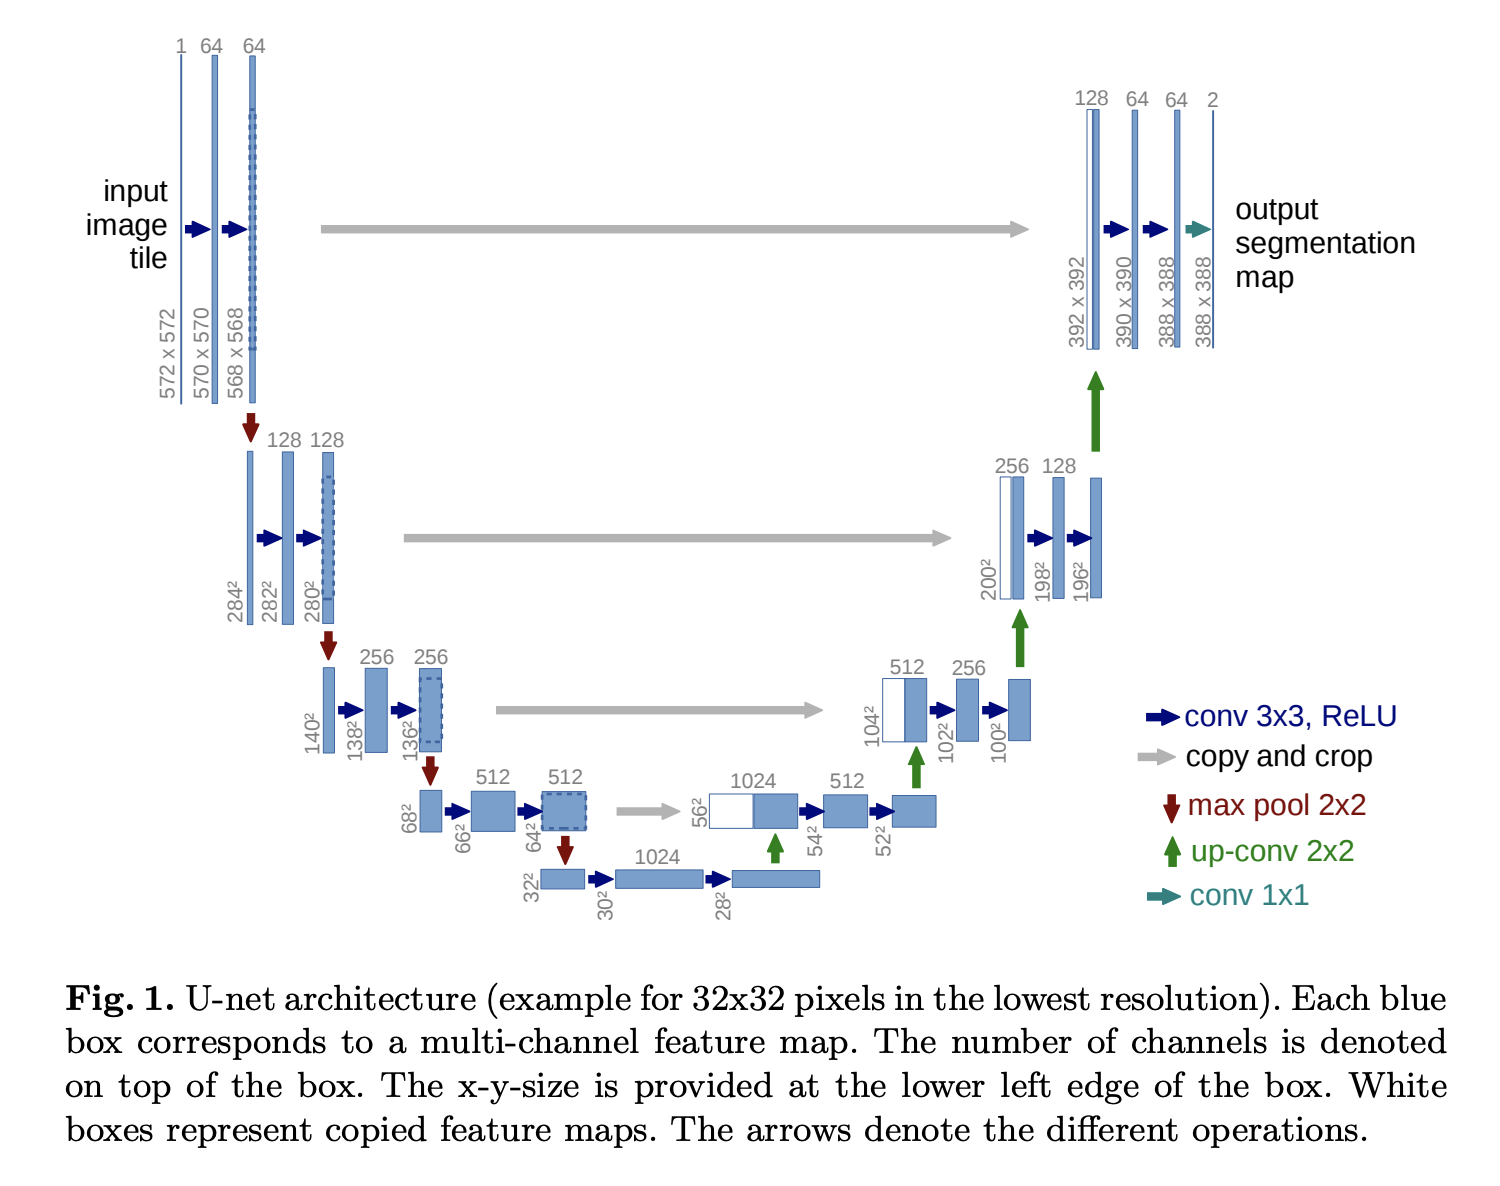
\includegraphics[scale=0.6]{images/1.png}
\subsection{Usecases of UNet Architecture}
The U-Net architecture is particularly useful for segmentation problems because it can effectively capture both local and global features. The encoder network can capture global features such as context and image-level information, while the decoder network can capture local features such as object boundaries and fine details. The skip connections help propagate information across the network, improving the accuracy of the segmentation. Additionally, the U-Net architecture is computationally efficient and can be trained on relatively small datasets, making it a practical choice for various segmentation tasks.
\begin{enumerate}
    \item High Accuracy: The U-Net model has shown to achieve high accuracy in various image segmentation tasks, including medical image segmentation and object detection in satellite imagery.
    \item Efficient use of data: The architecture makes efficient use of the available training data by utilizing the skip connections. The skip connections allow the network to combine low-level and high-level features, which helps in reducing the problem of vanishing gradients.
    \item Reduced Overfitting: The architecture uses data augmentation techniques, such as flipping, rotating, and zooming, which helps in preventing overfitting.
    \item Fast and Easy Training: The architecture is relatively easy to train, and training times are faster compared to other complex architectures.
\end{enumerate}


\chapter{Software Requirements Specification}

	
	\begin{flushright}
		\rule{16cm}{5pt}\vskip1cm
		\begin{bfseries}
			\Huge{}\\
			\vspace{0.5cm}
			for\\
			\vspace{1.5cm}
			Object Detection using Google Earth \\
			\vspace{1.5cm}
			\LARGE{Version 1.2 \myversion}\\
			\vspace{1.5cm}
			Prepared by : SujayKumar Reddy M (20BDS0294)\\
			\vspace{1.5cm}
			Sahaaya Arul Mary S.A
		\end{bfseries}
	\end{flushright}
	
	
	\section{Introduction}
	
	\subsection{Purpose}
	The usage of \textbf{Google Earth} and \textbf{Google Street View} is not very habitated by the users. In fact we can do many things for example Detecting Rooftops, Detection of more Heavy Vehicles to reduce the Pollution, in these applications this  product is specifically intended for. As when the Vehicle is in transit we cannot  track the vehicle in google earth because google earth is a satelite imagery where we cannot watch live changes.According to my research the google earth satellite imagery updates the images for every 1 to 3 years and NASA's Livestat project updates for every 16 days. This application is very much useful for drones to detect the roof-tops and all other Static Objects.My tool will be an interface for the research community for analyzing the vegetation in a particular area within a period of 2-3 years and Rooftop Detection for the drones to deploy a model and other various static applications. My tool will be an interface for all the entities which are available and they can use this to detect the produced Objects and this is the main concept of my model/tool.
	
	% This is very much difficult to maintain all the data of a course as a hard copy. Any data can be changed, deleted, added at any time. Such as - A new teacher can be assigned for a course, he also can be changed ; And so many student are getting admitted every semester. So, "IICT WEBSITE" is the solution. "IICT WEBSITE" is a official website based on marking and resulting system of IICT authorized. The main concept of "IICT WEBSITE" is to devitalized PGD, MIT courses, their students and teachers data maintenance. 
	%
	
	
	\section{Document Conventions}
	\begin{tabular}{ p{4.5cm} p{8cm} }
		
		
		GEE         &Its an API Service by Google named as Google Earth Engine.\\\\
		GSV         &Google Street View is an API Service Provided by the GEE and it mainly concentrates on Street Photography useful for AR/VR Apps \\\\
		Static Objects  &The Object which cannot be changed over 2-3 years of time like Buildings, farms and Vegetation within a particular reach.\\\\
		Tflite		&An Tensorflow Model which is used to Generate the Supervised Learning Approach for the Static Object Detection\\\\
				
		
		
	\end{tabular}
	
	
	\section{Intended Audience and Reading Suggestions}
	This Software Requirement Specification is for Myself for the future reference, Professor and testers.This SRS is done according to the template given by the Professor. Issues List is provided at the end of the document at Appendix C. Further, the discussion will provide all the internal, external, functional, and also non-functional information about "Object Detection from Google Earth Images". 
	
	
	
	
	
	
	
	
	\section{Project Scope}
	The Major Stakeholders are the ... 
	\begin{enumerate}
		\item User
		\item GEE
		\item Object Identification
		\item Time
		\item Tracking 
	\end{enumerate}
	GEE will take care with the communication of the satellites and takes in the data of satellite image processing. We will only consider that processed image as the input to our model or tool. The GEE API Service will give us an API Services where we can navigate for a zommed in image to process the image carefully. The Service would be connected with our System which will detect the Objects and track the motion of the detected object.
	\newline
	Object Identification is an Machine Learning Model which detects the objects by Open CV2 it marks the object and classifies as an provided class label.
	\newline
	The User communicates with the GEE Service through our interface and gives us the starting co-ordinates and starting image to identify.
	\newline
	The Time is important because we are considering the static imagery of the Google Earth Engine. We need the images which are useful for real time data by using various sensors but the dataset which we use to train our data.
	\newline
	\begin{center}
		\begin{figure}
			\centering
			\includegraphics[scale=0.32]{images/2.png}
			\caption{Entire work-flow}
			\label{}
		\end{figure}
	\end{center}
	
	Figure 1.1 (Entire work-flow) is the overview of the project. Connection of all the entities are dependable to each others.  This gives the simple idea about the functional activities of the project. 
	\newline
	Google Earth Engine will be a static input for our web application because the model which we trained for.
	\newline
	So, every entity is vary much interactive with each other.
	
	The project scope for Object Detection from Google Earth Images would typically include the following:
	
	\begin{enumerate}
		\item Object Detection Algorithm: Develop a computer vision algorithm to detect objects in Google Earth images using techniques such as convolutional neural networks (CNNs), region-based convolutional neural networks (R-CNNs), and You Only Look Once (YOLO) algorithms.
		\item Image Dataset: Create or obtain a dataset of Google Earth images for training and testing the object detection algorithm. The dataset should include a variety of different objects in different environments and under different conditions.
		\item Model Training: Train the object detection algorithm using the image dataset. This will involve adjusting the parameters and architecture of the model until it can accurately detect objects in the images.
		\item Model Deployment: Integrate the trained object detection model into an application that can be used to process Google Earth images and detect objects within them.
		\item User Interface: Develop a user interface that allows users to select an image from Google Earth, process it with the object detection model, and view the results. The interface should be intuitive and easy to use.
		\item Performance Evaluation: Evaluate the performance of the object detection model by comparing its results to a ground truth dataset. This will involve measuring metrics such as precision, recall, and accuracy.
		\item Optimization: Optimize the performance of the object detection model by making changes to the algorithm, dataset, or other aspects of the system as necessary.
	\end{enumerate}
	
	
	% \section{References}
	% \url{}{}
	
	
	
	
	
	
	
	
	
	
	
	
	
	
	
	
	
	\section{Overall Description}
	
	\subsection{Product Perspective}
	Google earth is a large system and My Tool integrates into this particular API Services for providing various analysis of geo-spatial data. Main goal of this project is to minimize the workflow of using drones to calculate the static data instead we can use our tool to Identify the static objects for data analysis.
	
	
	
	
	
	
	
	
	
	\subsection{User Classes and Characteristics}
	This Object Detection has basically 2 types of users. 
	\begin{itemize}
		\item Researchers
		\item Business Entitites 
	\end{itemize}
	The Researchers working on SOLAR Energy they have the very useful application to know how much area does the each village has so we can implement it by comparatively.\\\\
	The Business Entities like Amazon can use the models to detect the rooftops to deliver the packages for per user.
	% \begin{figure}
		%     \centering
		%     \includegraphics[width=10cm]{2.JPG}
		%     \caption{type of users}
		%     \label{fig:type of users}
		% \end{figure}
	
	\subsection{Product Functions}
	The Product should be able to detect the rooftops for the drones in-order to land the package for asset management services. If the Object is the Farming Lands then the Drone would find the optimal point where all the agriculture sensors would be able to communicate within the distance.
	
	Before using the main function of the software result process, users have to be registered. 
	\newline
	The Products primary source is the Machine Learning model. Result is the main feature of all. It contains the Object which is marked by the Open CV2.
	
	\subsection{Operating Environment}
	The website will be operate in any Operating Environment - Mac, Windows, Linux etc. 
	
	\subsection{Design and Implementation Constraints}
	As the ML model is the primary source we consider that as a Design.
	\begin{itemize}
		\item From the Unprocessed Image from the GE.
		\item Supervised Learning Techniques.
		\item Class Labels and Unsupervised Learning Techniques.\\
	\end{itemize}


	From the GE Image we need to detect the static objects and find a suitable environment with color grading which would provide us an Undefined colored so, it acn be easily seen by the Sensors or Microcontrollers in the Drones.\\
	
	Every Image would happen to work with utmost accuracy to detect the static images.\\\\
	
	Design and implementation constraints for object detection from Google Earth can vary depending on the specific use case and requirements. However, some common constraints and considerations are:

	

	

	\begin{itemize}
		\item Image Quality: The quality and resolution of the satellite images in Google Earth can have a significant impact on the accuracy and reliability of object detection. Poor quality images with low resolution, or images that are obstructed by clouds or other factors, can make it difficult to accurately detect objects.
		\item Object Variability: The variability of objects in satellite images can also impact the accuracy and reliability of object detection. Objects may vary in size, shape, orientation, and appearance, which can make it challenging to train object detection algorithms to recognize them.
		\item Computational Resources: Object detection can be computationally intensive, and large amounts of data need to be processed in real-time to ensure fast and accurate results. It is important to carefully consider the computational resources required to run the object detection algorithm, as well as the hardware and software infrastructure required to support it.
		\item Data Privacy and Security: Google Earth images may contain sensitive information that needs to be protected, and it is important to ensure that the object detection algorithm is designed and implemented in a way that protects this information.
		\item Data Storage and Management: The amount of data generated by object detection from Google Earth images can be large, and it is important to have a robust and scalable data storage and management system in place to handle this data.
	\end{itemize}

These are some of the key design and implementation constraints for object detection from Google Earth. However, there may be additional constraints and considerations that are specific to your use case and requirements.
	
	
	
	
	
	
	
	
	
	
	
	
	
	
	\section{System Features}
	
	
	
	\subsection{Functional Requirements}
	\begin{enumerate}
		\item The object detection software should be able to process images from Google Earth and extract relevant information for object detection. This may involve implementing algorithms for image pre-processing, such as image resizing, and image normalization.
		\item The object detection software should be able to detect objects of interest in the images, such as buildings, vehicles, and roadways. This may involve implementing object detection algorithms, such as deep learning-based object detection, and training the algorithms on annotated image data.
		\item The object detection software should be able to classify the objects detected in the images into relevant categories, such as type of building, type of vehicle, or type of roadway. This may involve implementing object classification algorithms and training the algorithms on annotated image data.
		\item The object detection software should be able to locate the objects in the images and provide the coordinates of the objects. This may involve implementing object localization algorithms, such as bounding box regression, and training the algorithms on annotated image data.
		\item The object detection software should be able to generate outputs, such as annotated images or data reports, that provide information about the objects detected in the images. This may involve implementing output generation algorithms and user interfaces for visualizing the outputs.
		\item The object detection software should provide user interfaces for interacting with the software, such as uploading images, configuring the object detection algorithms, and viewing the outputs. This may involve implementing graphical user interfaces, command line interfaces, or application programming interfaces (APIs) for integrating the object detection software with other software systems.
	\end{enumerate}
	
	
	
	
	
	
	
	\section{External Interface Requirements}
	TensorFlow Lite (TFLite) is a lightweight version of TensorFlow, designed to run on resource-constrained devices such as mobile phones and embedded systems. The TFLite object detection model can be integrated into various external user interfaces to provide object detection capabilities to end users. Some common external user interfaces for TFLite object detection models are:
	\begin{enumerate}
		\item Mobile Applications
		\item Web Applications
		\item Embedded Systems.
		\item Robotics
	\end{enumerate}
These are some of the external user interfaces that TFLite object detection models can be integrated with. The specific user interface that you choose will depend on your use case and requirements. It is important to carefully consider the requirements of your application and the resources available on your target device when selecting an external user interface for your TFLite object detection model.

\subsection{Software Interfaces}
\begin{enumerate}
	\item Mobile SDKs: TFLite object detection models can be integrated into mobile software development kits (SDKs), allowing developers to build mobile applications that perform object detection on mobile devices.
	\item Web API: TFLite object detection models can be deployed as web APIs, allowing object detection to be performed over the internet. This can be useful for building cloud-based object detection systems that can be accessed by a variety of clients, such as mobile applications, web applications, and desktop applications.
	\item Robotics API: TFLite object detection models can also be integrated into robotics APIs to provide object detection capabilities for autonomous robots.
	\item Embedded API: TFLite object detection models can be integrated into embedded APIs, allowing developers to build custom embedded systems that perform object detection.
	 
\end{enumerate}

\subsection{Hardware Interfaces}
The Google Earth API can be integrated with various hardware interfaces to provide mapping and visualization capabilities to end users. Some common hardware interfaces for the Google Earth API are:
\begin{enumerate}
\item Web Browsers: The Google Earth API can be integrated into web browsers to provide interactive mapping and visualization capabilities to end users. This allows users to access Google Earth in their web browsers and interact with maps and satellite imagery.
\item Embedded Systems: The Google Earth API can be integrated into embedded systems, such as GPS devices and in-vehicle navigation systems, to provide mapping and visualization capabilities in these environments.
\item Robotics Hardware: The Google Earth API can also be integrated into robotics hardware, such as autonomous robots, to provide mapping and navigation capabilities for these systems.
	
\end{enumerate}
These are some of the hardware interfaces that the Google Earth API can be integrated with. The specific hardware interface that you choose will depend on your use case and requirements. It is important to carefully consider the requirements of your application and the resources available on your target device when selecting a hardware interface for the Google Earth API.


	\section{Other Nonfunctional Requirements}
	
	\subsection{Performance Requirements}
	The performance requirements for object detection from Google Earth images will depend on a number of factors, including the size of the images, the complexity of the objects being detected, the desired accuracy and speed of the object detection process, and the resources available on the hardware platform where the object detection is being performed. Some of the key performance requirements for object detection from Google Earth images include:
	\begin{enumerate}
		\item Computational Power: Object detection algorithms can be computationally intensive, and therefore a powerful processing platform is necessary to perform object detection in real-time. This may involve using high-performance CPUs, GPUs, or other specialized hardware such as Tensor Processing Units (TPUs).
		\item Memory: Object detection algorithms require large amounts of memory to store the image data and intermediate results of the object detection process. Therefore, the hardware platform should have sufficient memory to support the object detection process.
		\item Network Bandwidth: If the object detection is being performed in a cloud environment, the network bandwidth between the cloud and the client device may also be a factor in the performance of the object detection process.
		\item Latency: The latency of the object detection process is an important factor in the overall performance of the system. Latency refers to the time it takes for an object detection request to be processed and the results to be returned to the client. Low latency is important for real-time applications where the results of the object detection process need to be available immediately.
		\item Accuracy: The accuracy of the object detection process is also a critical factor in the overall performance of the system. High accuracy is important for applications where the object detection results are used to make important decisions, such as in autonomous vehicles or surveillance systems. 
	\end{enumerate}
These are some of the key performance requirements for object detection from Google Earth images. The specific performance requirements for your application will depend on the details of your use case and the desired outcomes. It is important to carefully consider the performance requirements of your application and the resources available on your hardware platform when designing and implementing an object detection system from Google Earth images.
	
	\subsection{Security Requirements}
	Security is an important consideration in any application that involves processing and storing sensitive information, including object detection from Google Earth images. Some of the key security requirements for object detection from Google Earth images include:
	
	\begin{enumerate}
		\item Data Privacy: The privacy of the image data being processed and stored must be protected. This may involve encrypting the image data and ensuring that it is only accessible by authorized individuals.
		\item Data Integrity: The integrity of the image data must be protected to prevent unauthorized changes to the data. This may involve implementing data integrity checks and audit trails to detect any unauthorized changes to the data.
		\item Access Control: Access to the image data and the object detection results must be controlled to ensure that only authorized individuals have access to the data. This may involve implementing user authentication and authorization mechanisms, such as usernames and passwords, to control access to the data.
		\item Network Security: The network over which the image data is transmitted and the object detection results are returned must be secure to prevent unauthorized access to the data. This may involve implementing encryption algorithms, such as SSL/TLS, to secure the data transmission.
		\item Physical Security: The hardware platform where the object detection is performed must be physically secured to prevent unauthorized access to the image data and the object detection results. This may involve implementing physical security measures, such as security cameras, access controls, and secure data storage facilities.
		
	\end{enumerate}
These are some of the key security requirements for object detection from Google Earth images. The specific security requirements for your application will depend on the sensitivity of the image data and the desired level of security. It is important to carefully consider the security requirements of your application and to implement appropriate security measures to protect the image data and the object detection results.

\subsection{Software Quality Attributes}
		Software quality attributes are characteristics of software that are important to ensure that the software is fit for its intended use. In the context of object detection from Google Earth images, some of the key software quality attributes include:
		\begin{enumerate}
			\item Usability: The object detection software should be easy to use and understand for the end-users. This may involve providing clear and concise user interfaces, user-friendly error messages, and intuitive navigation.
			\item Reliability: The object detection software should be reliable and should perform its intended functions accurately and consistently. This may involve implementing robust error handling mechanisms, redundant components, and regular software testing.
			\item Performance: The object detection software should perform efficiently and quickly, especially for real-time applications. This may involve optimizing the algorithms for the hardware platform, reducing latency, and improving computational performance.
			\item Scalability: The object detection software should be able to handle increasing volumes of image data and users without degradation in performance. This may involve implementing scalable algorithms and architectures, load balancing, and distributed computing.
			\item Maintainability: The object detection software should be maintainable, so that it can be updated and improved over time. This may involve writing clear and well-documented code, using modular design patterns, and following software development best practices.
		\end{enumerate}
	
	

	
	

\chapter{Diagrams in Software Engineering}
\section{Work Breakdown Structure}
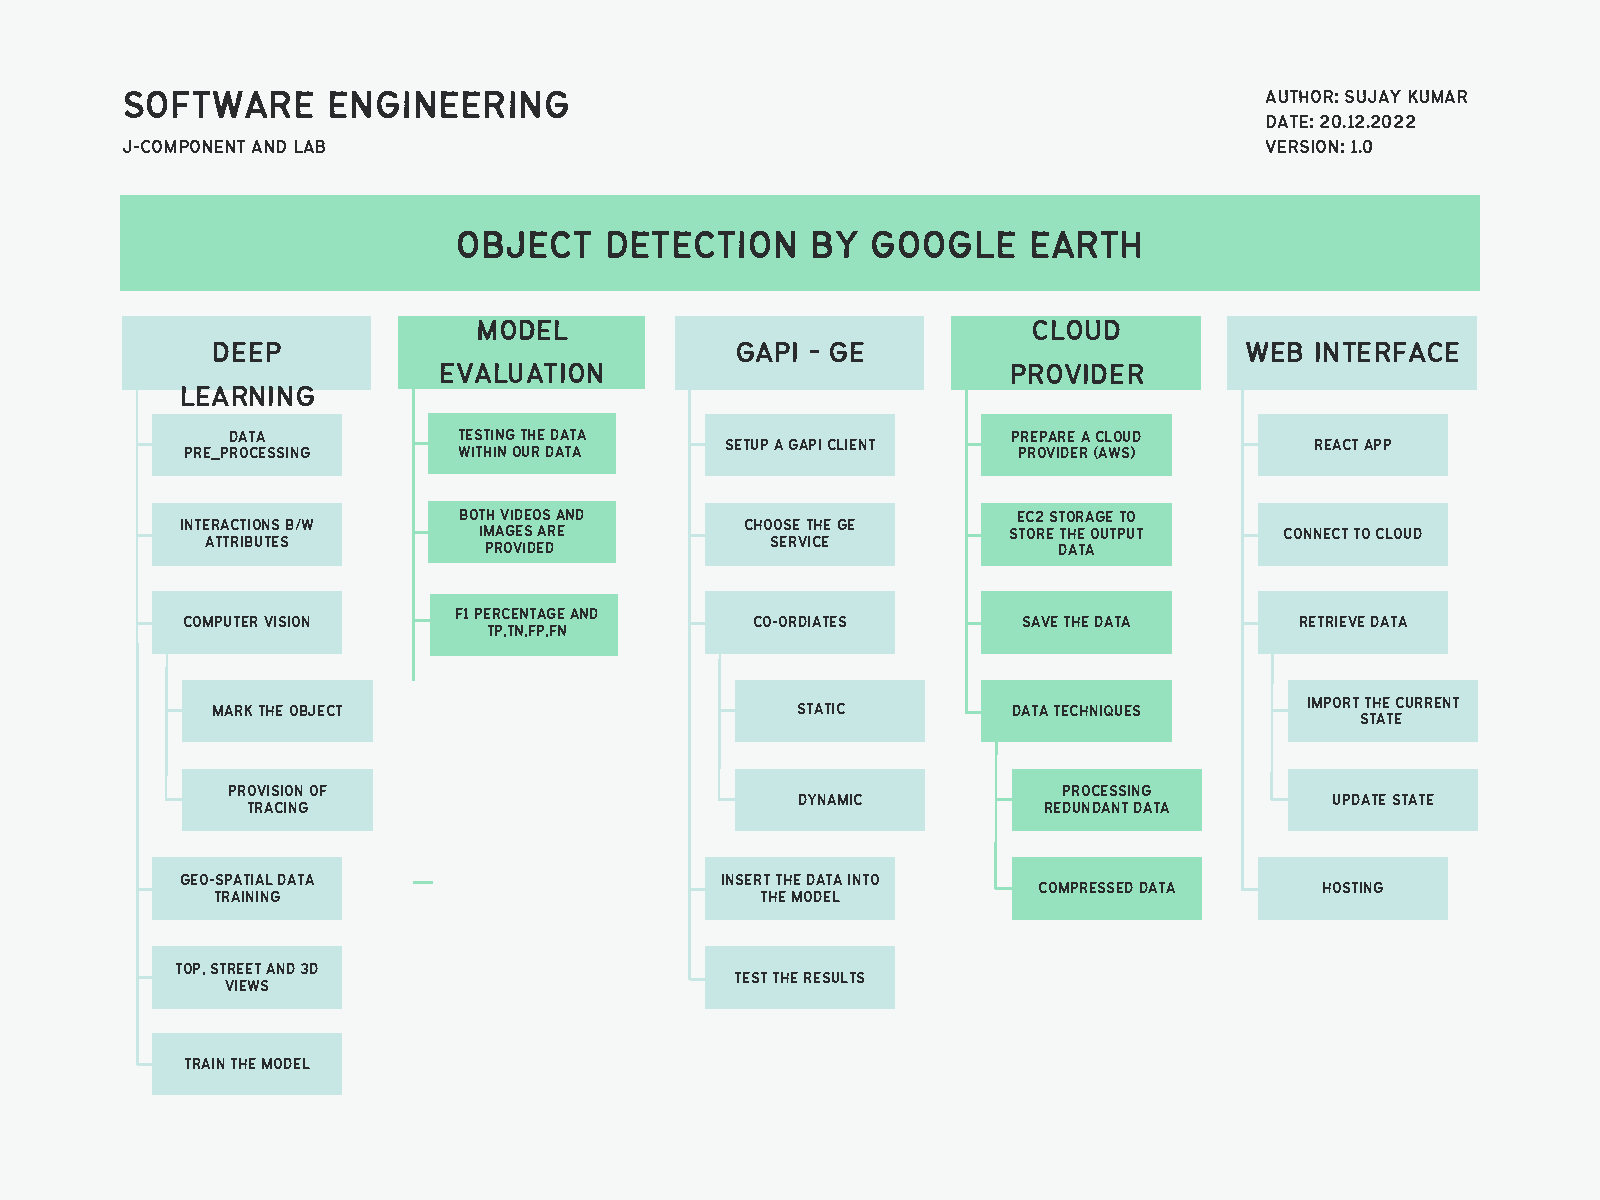
\includegraphics[scale=0.6]{images/wbs.pdf}
\section{Gantt Chart}
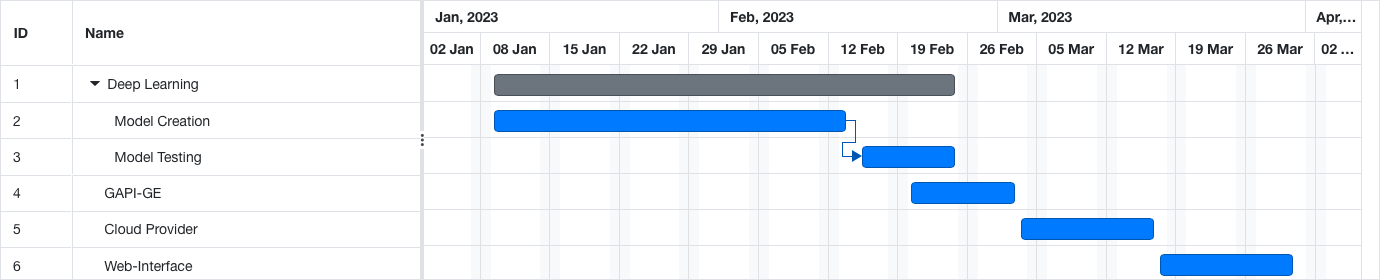
\includegraphics[scale=0.4]{images/gantt.png}
\section{DataFlow Diagram}
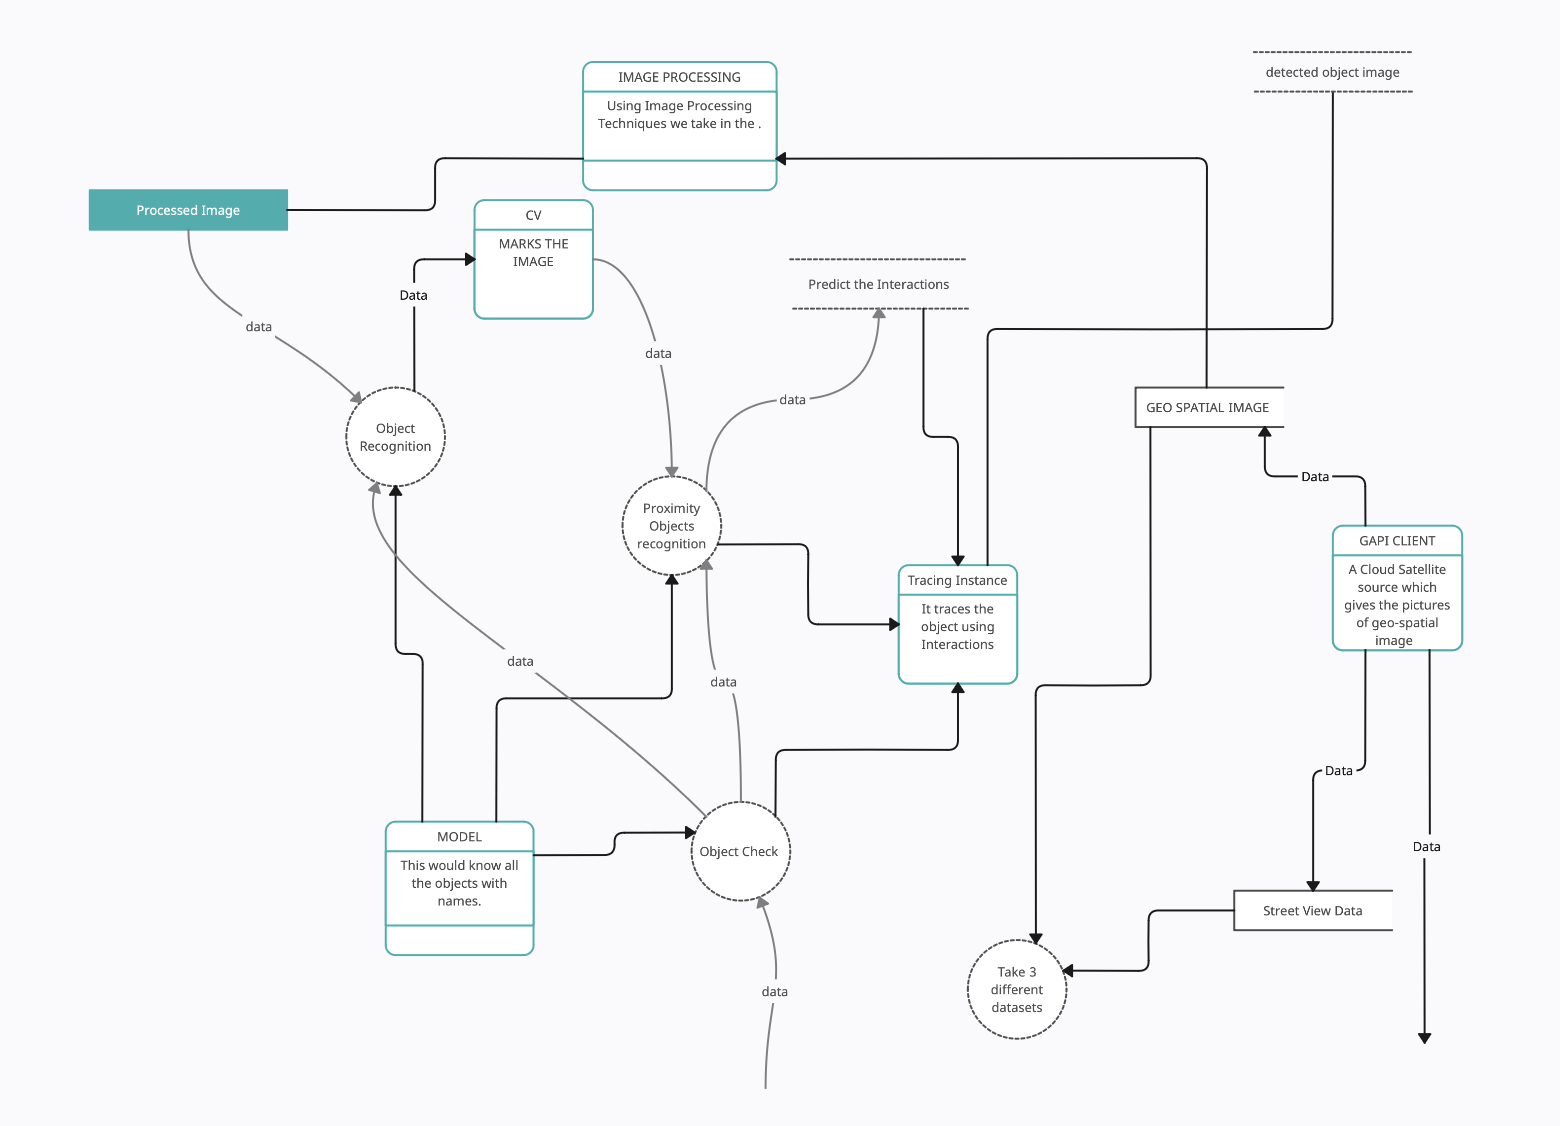
\includegraphics[scale=0.6]{images/dfd.png}
\section{ER Diagram}
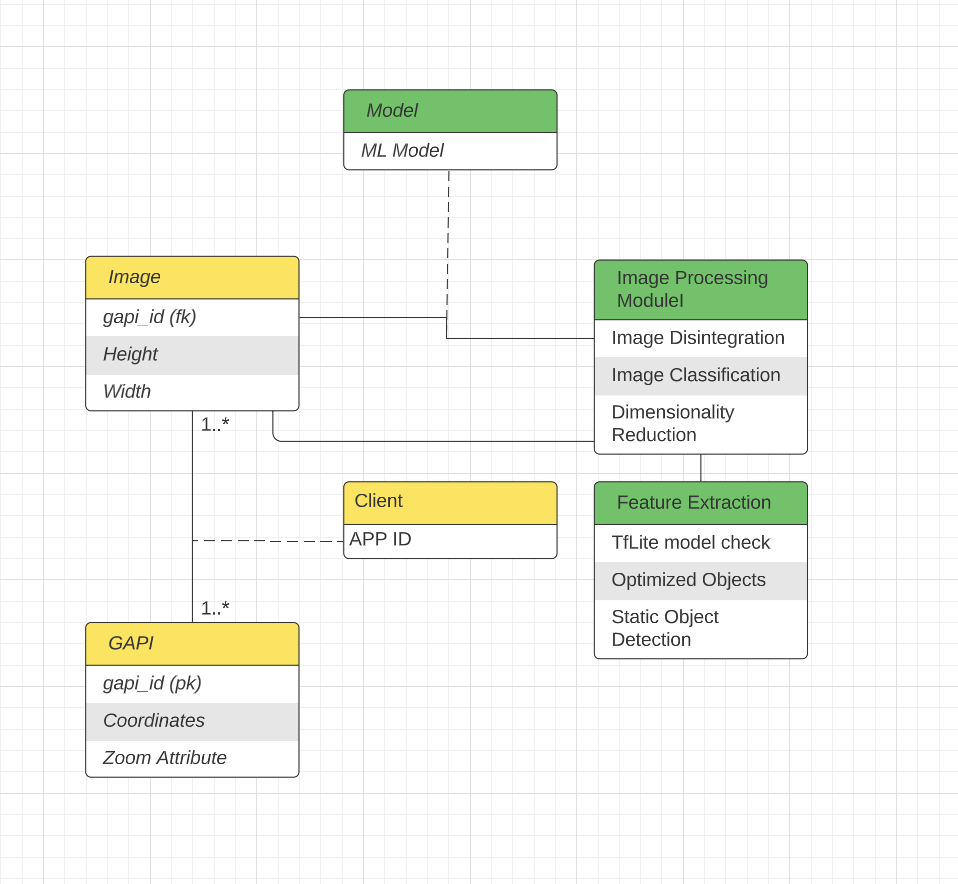
\includegraphics[scale=1.3]{images/er.png}
\section{Use Case Diagram}
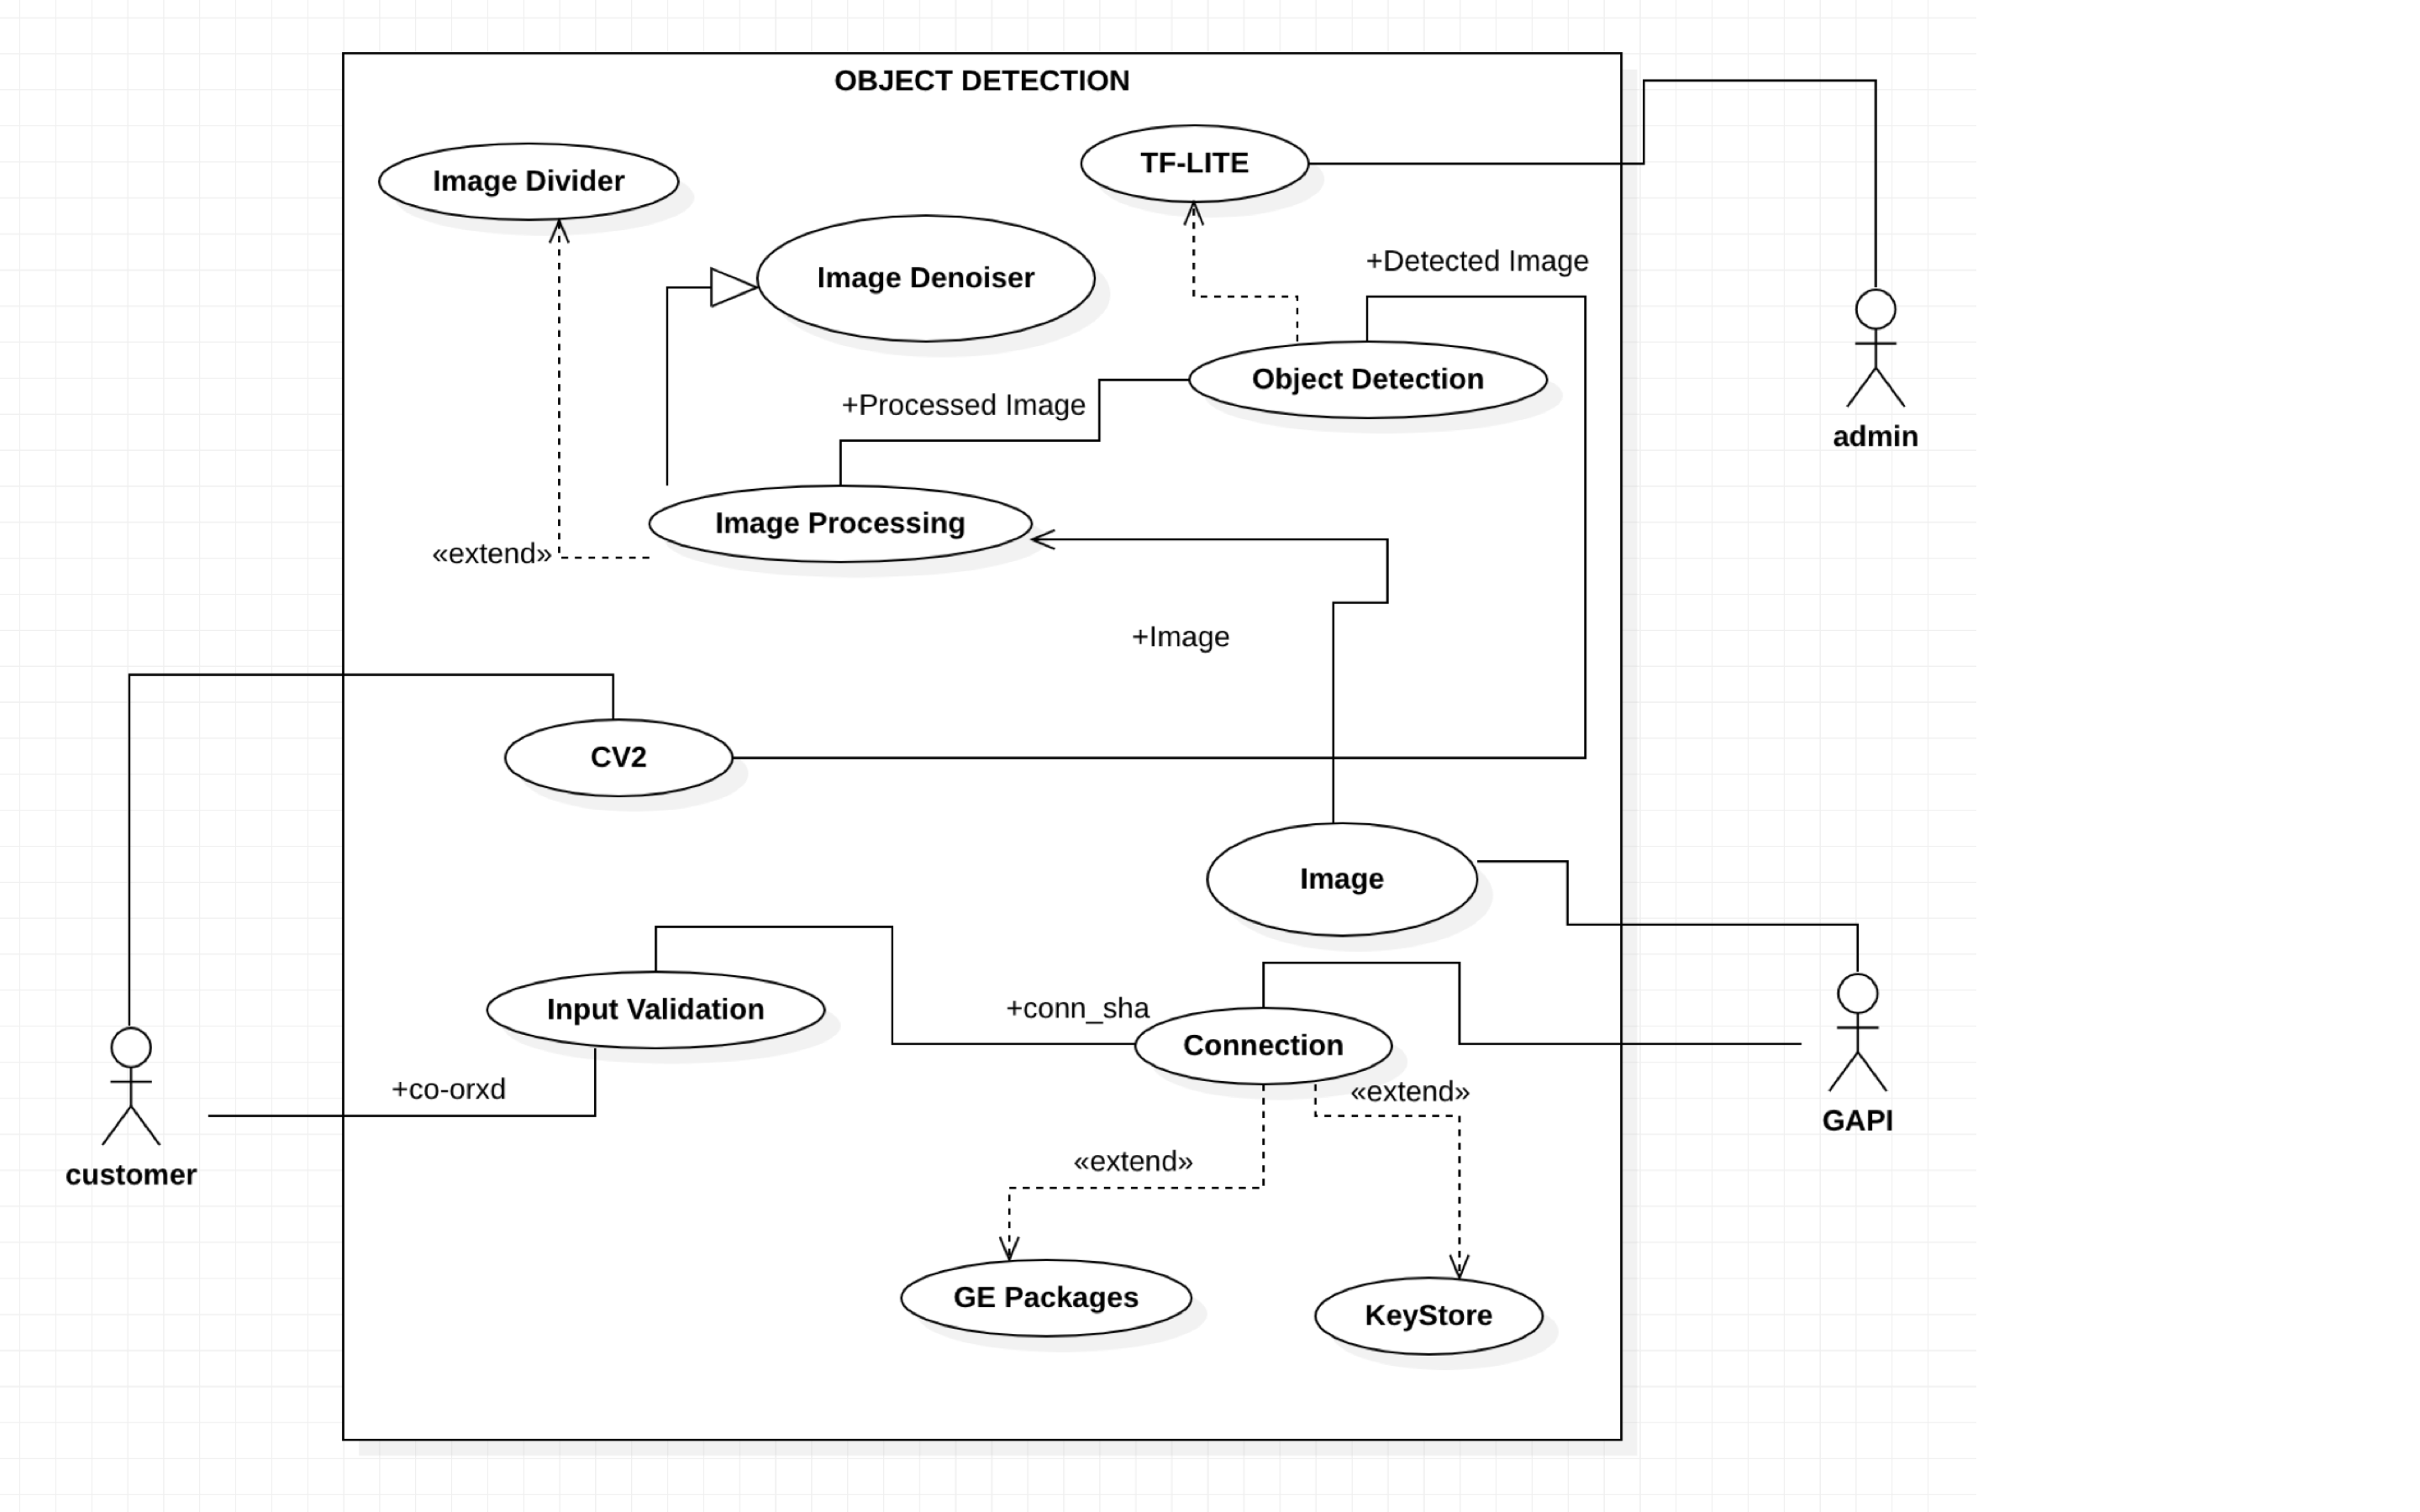
\includegraphics[scale=0.48]{images/usecase.png}
\section{Class Diagram}
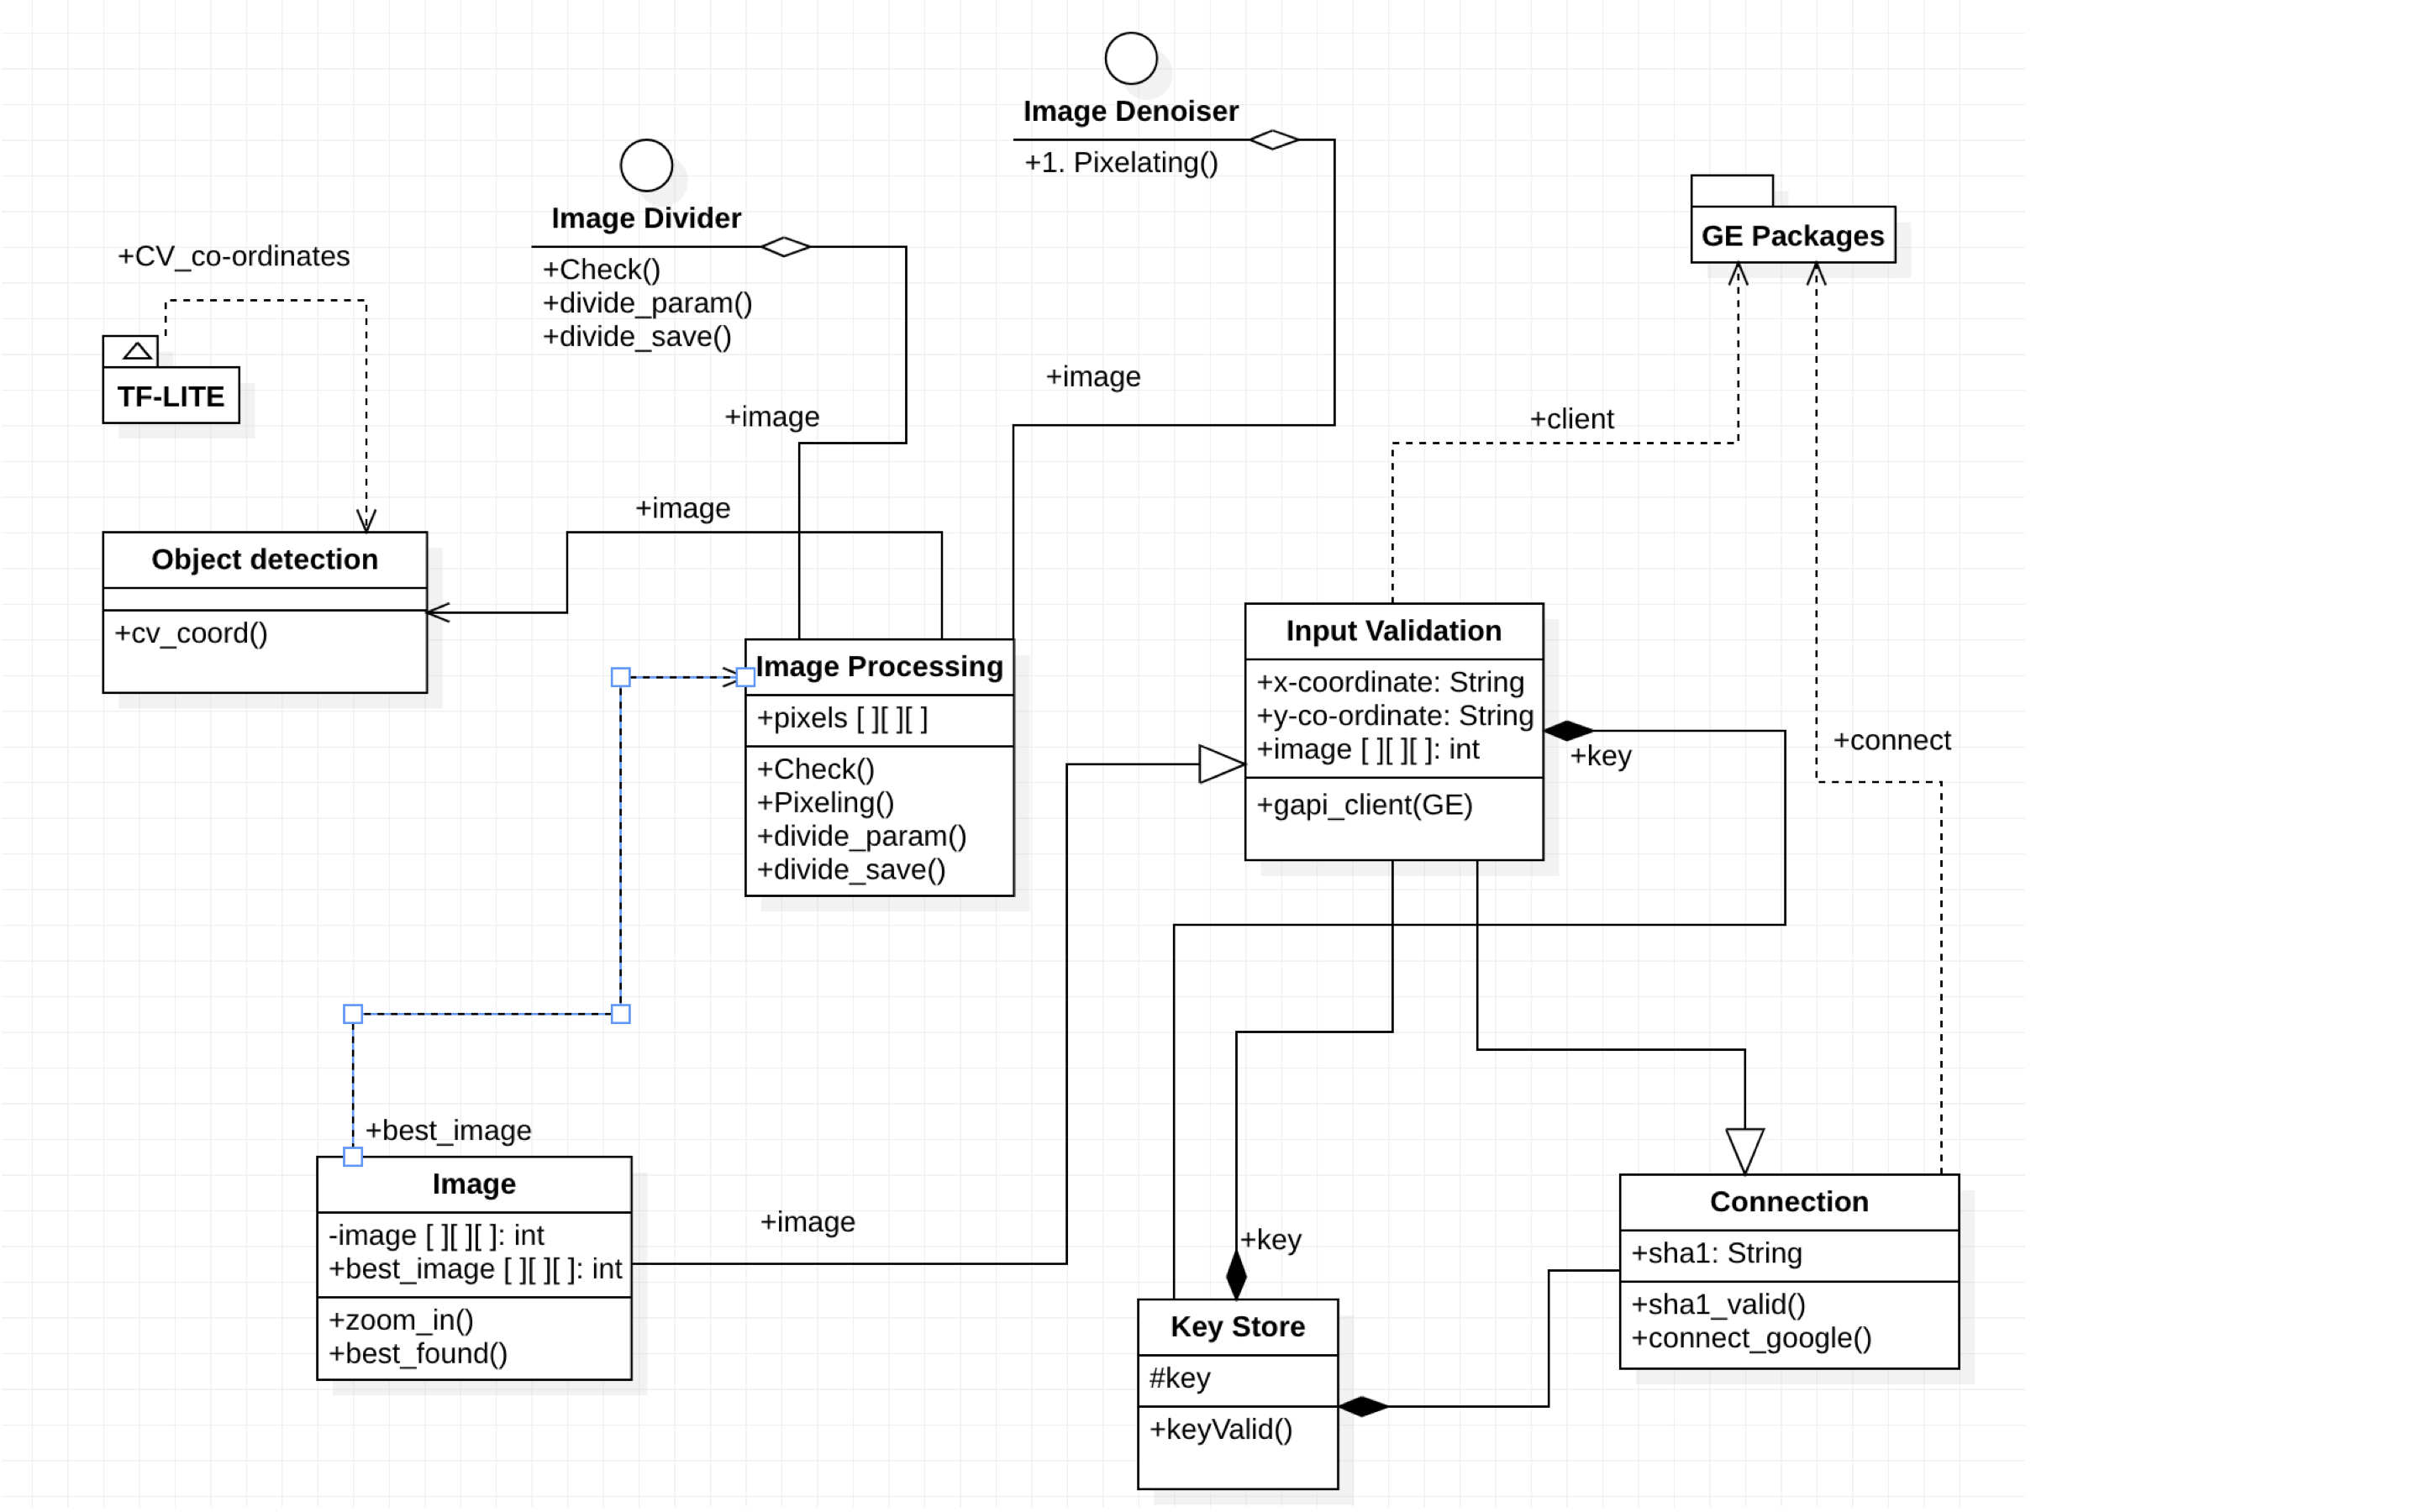
\includegraphics[scale=0.46]{images/class.png}
\section{Sequence Diagram}
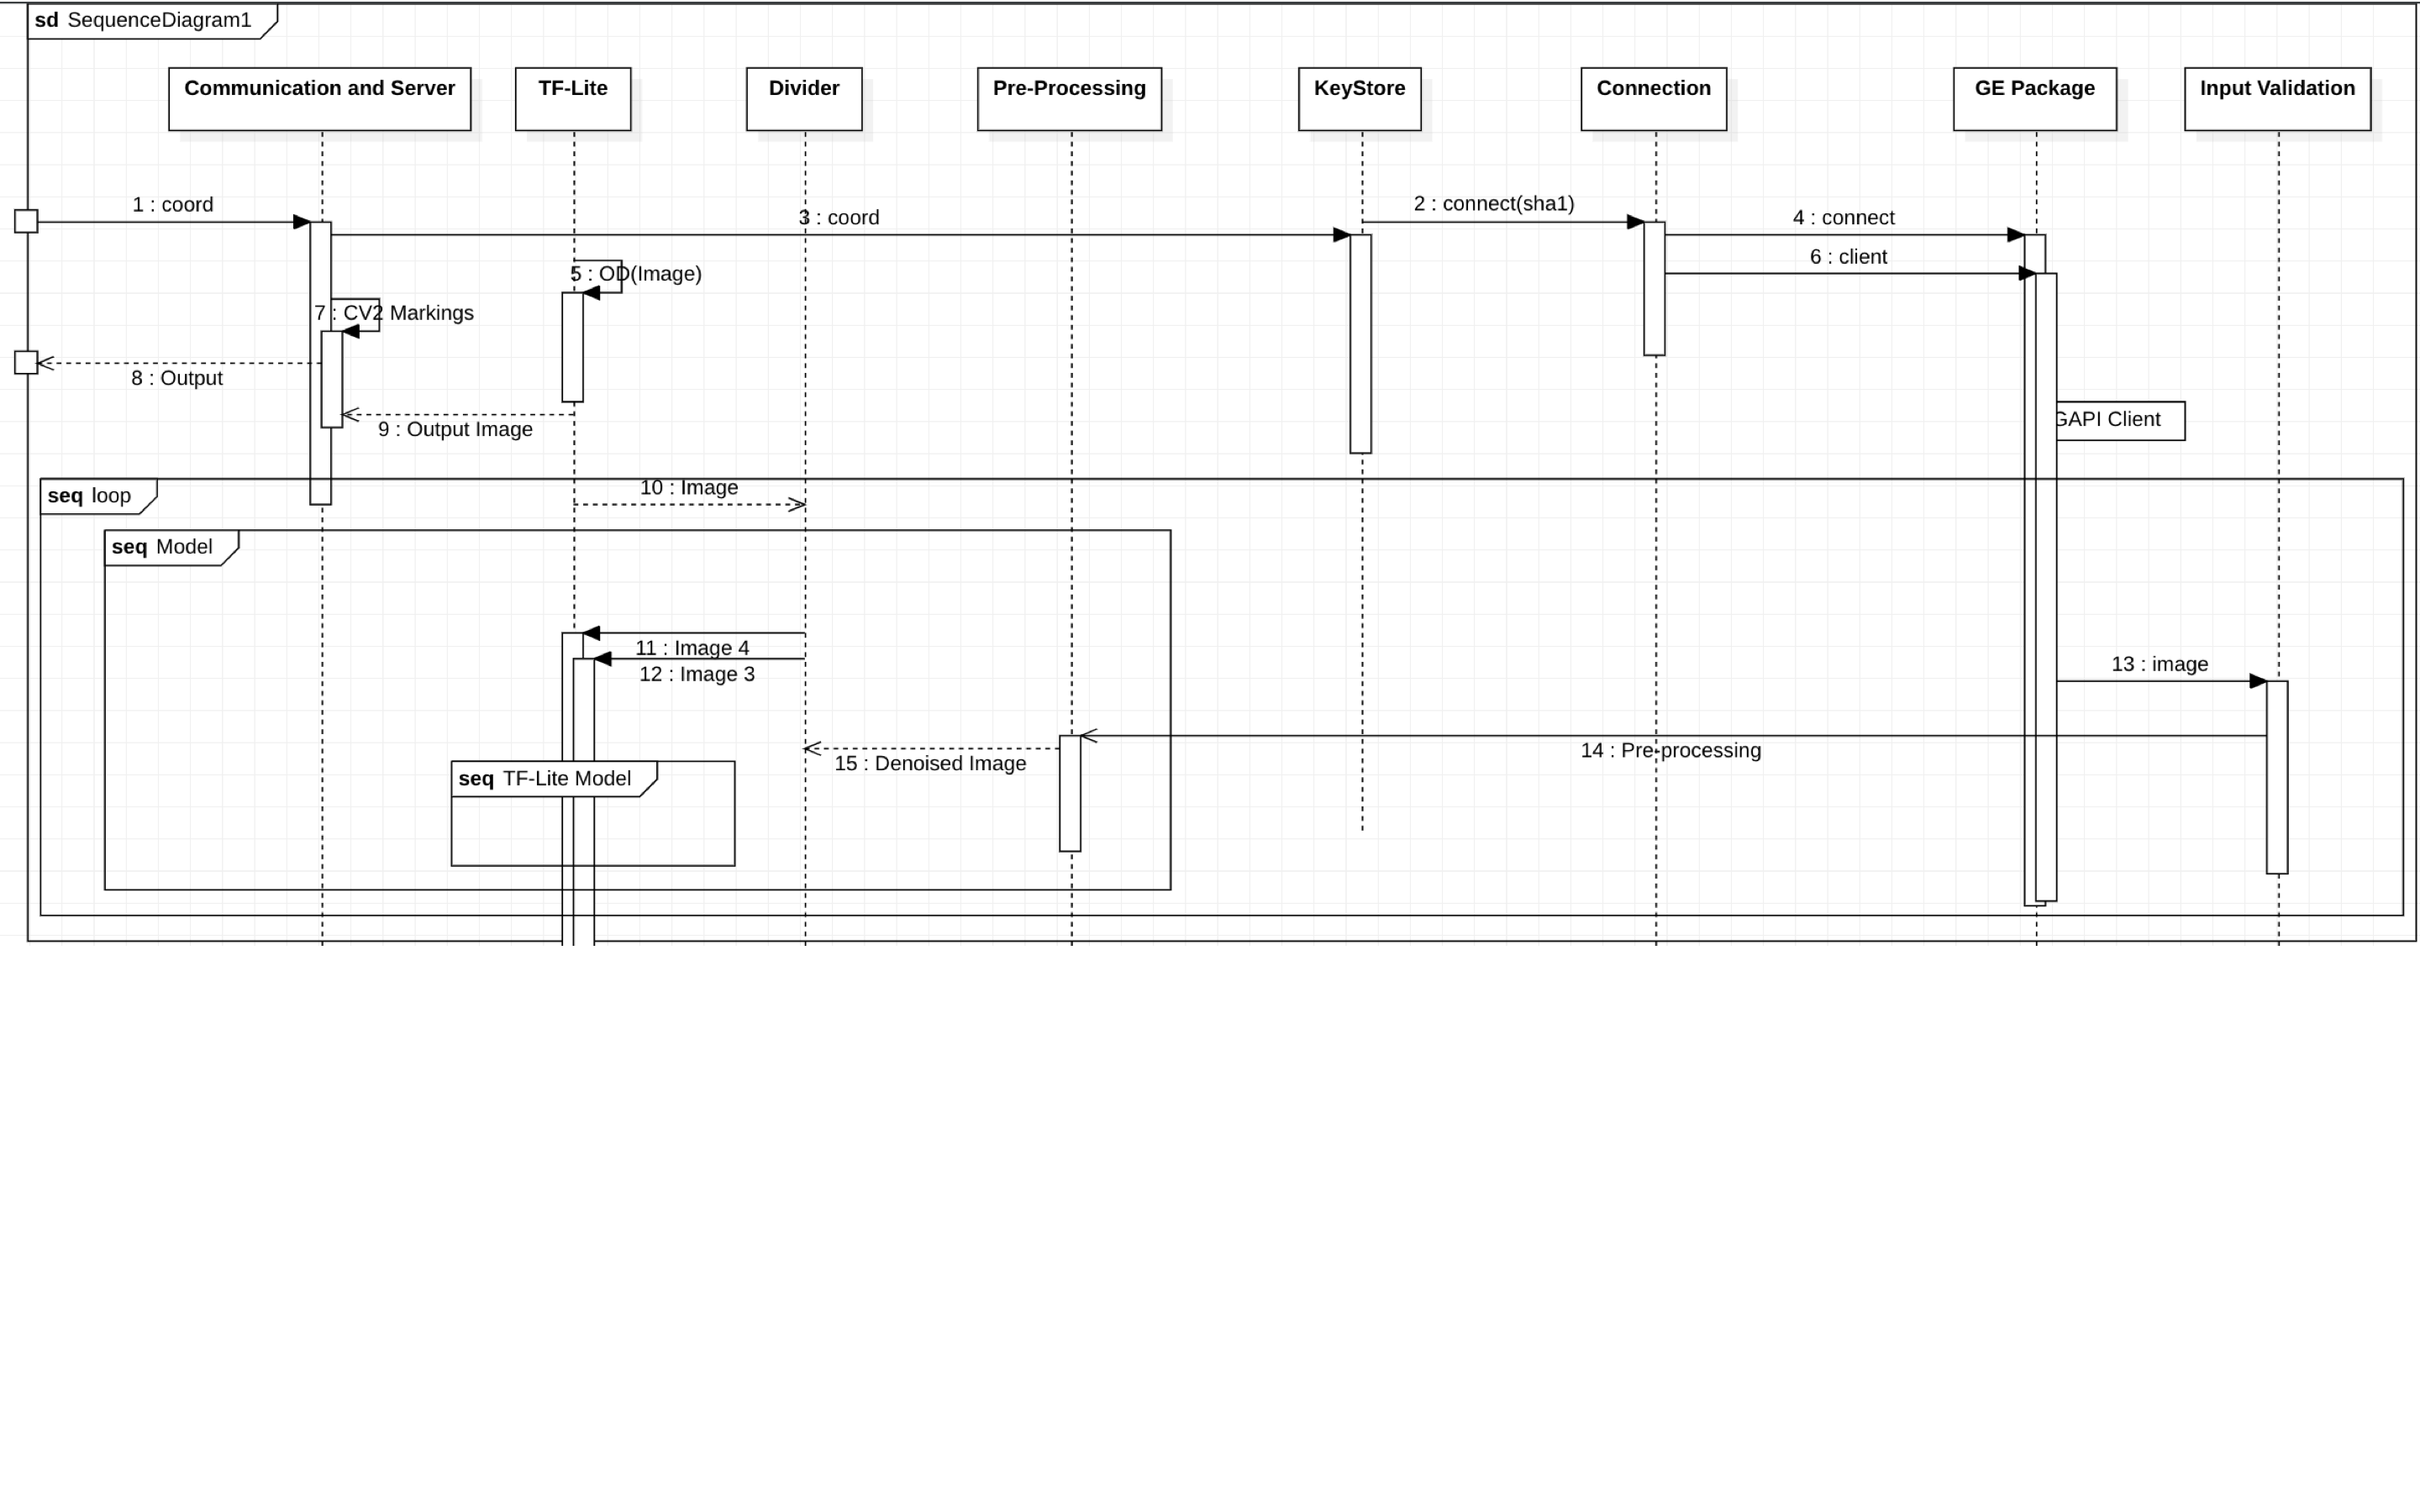
\includegraphics[scale=0.38]{images/seq.png}
\section{State Chart Diagram}
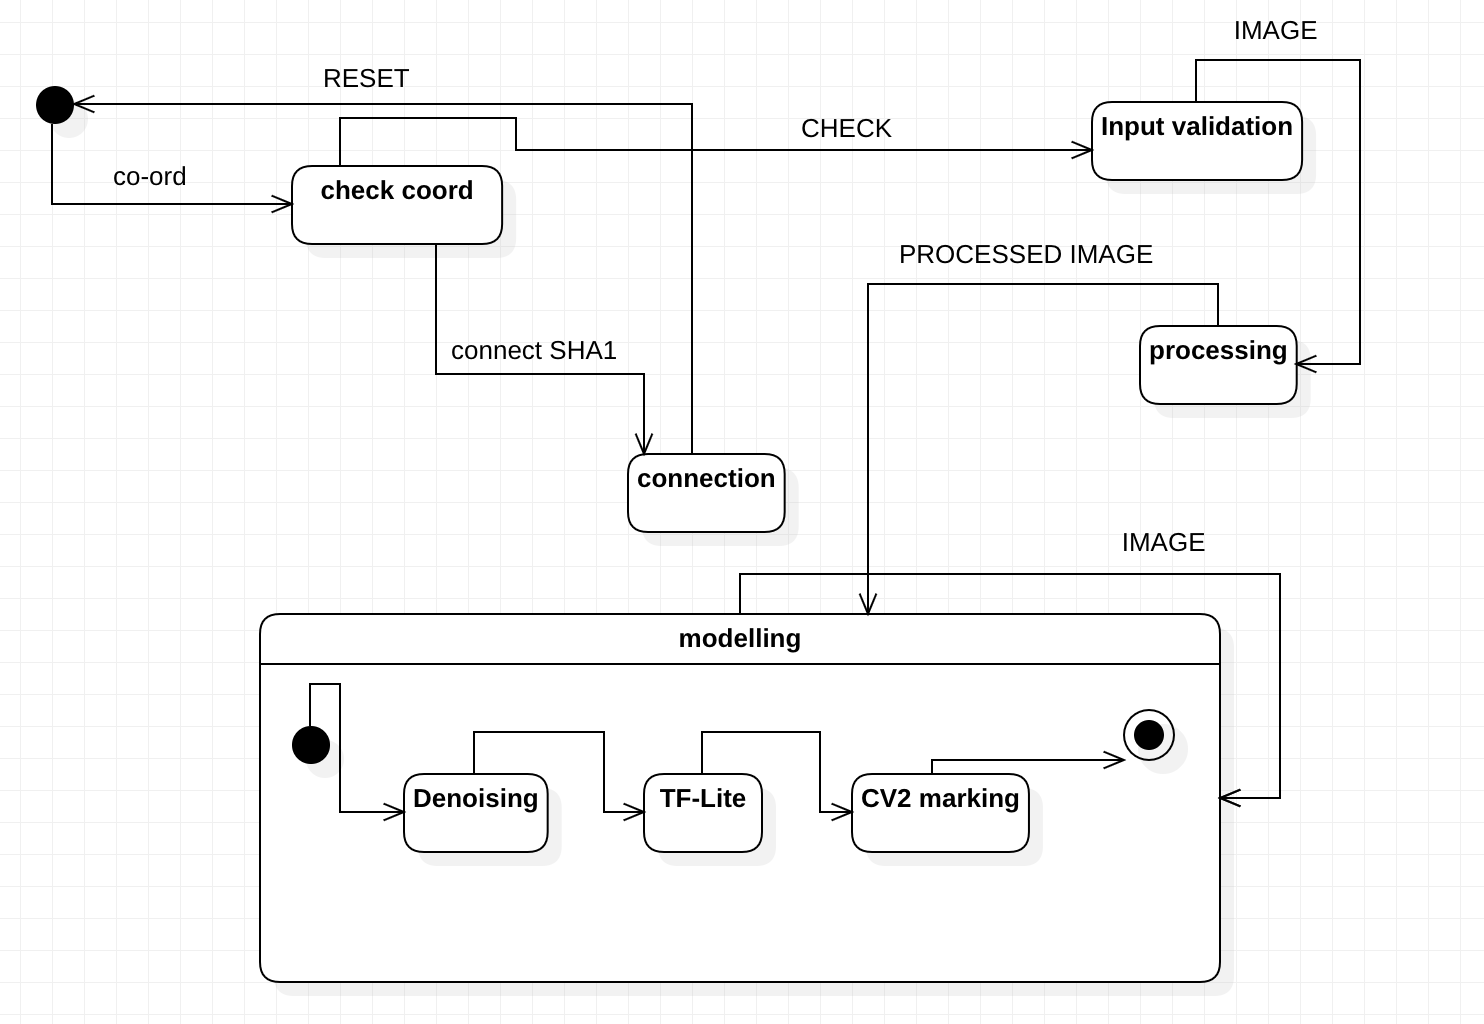
\includegraphics[scale=0.4]{images/statechart.png}
\section{Communication Diagram}
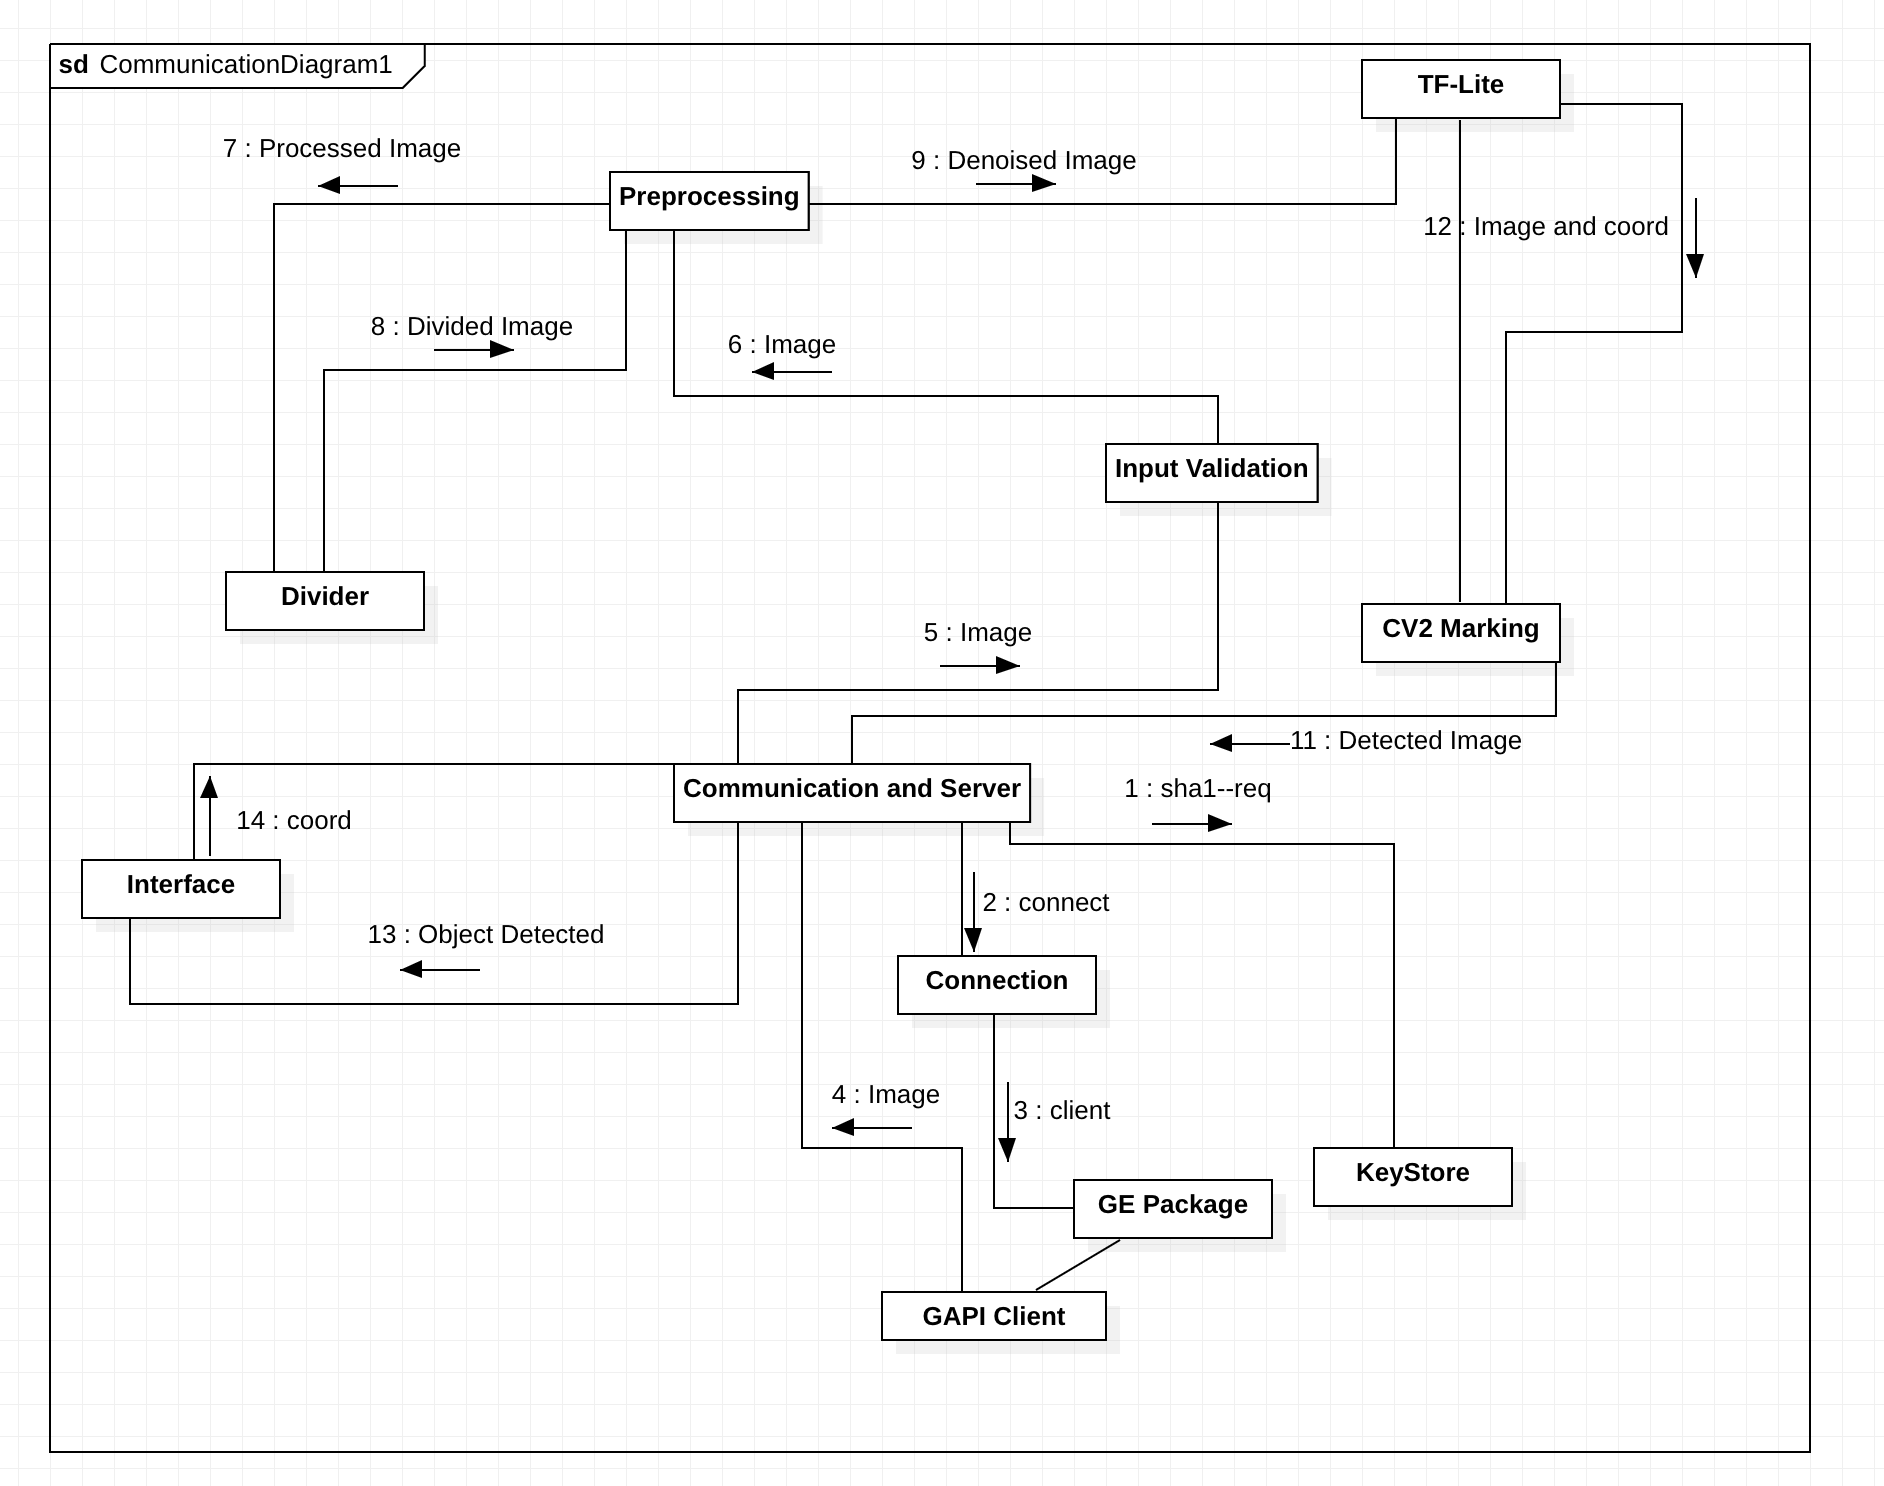
\includegraphics[scale=0.6]{images/com.png}
\section{Activity Diagram}
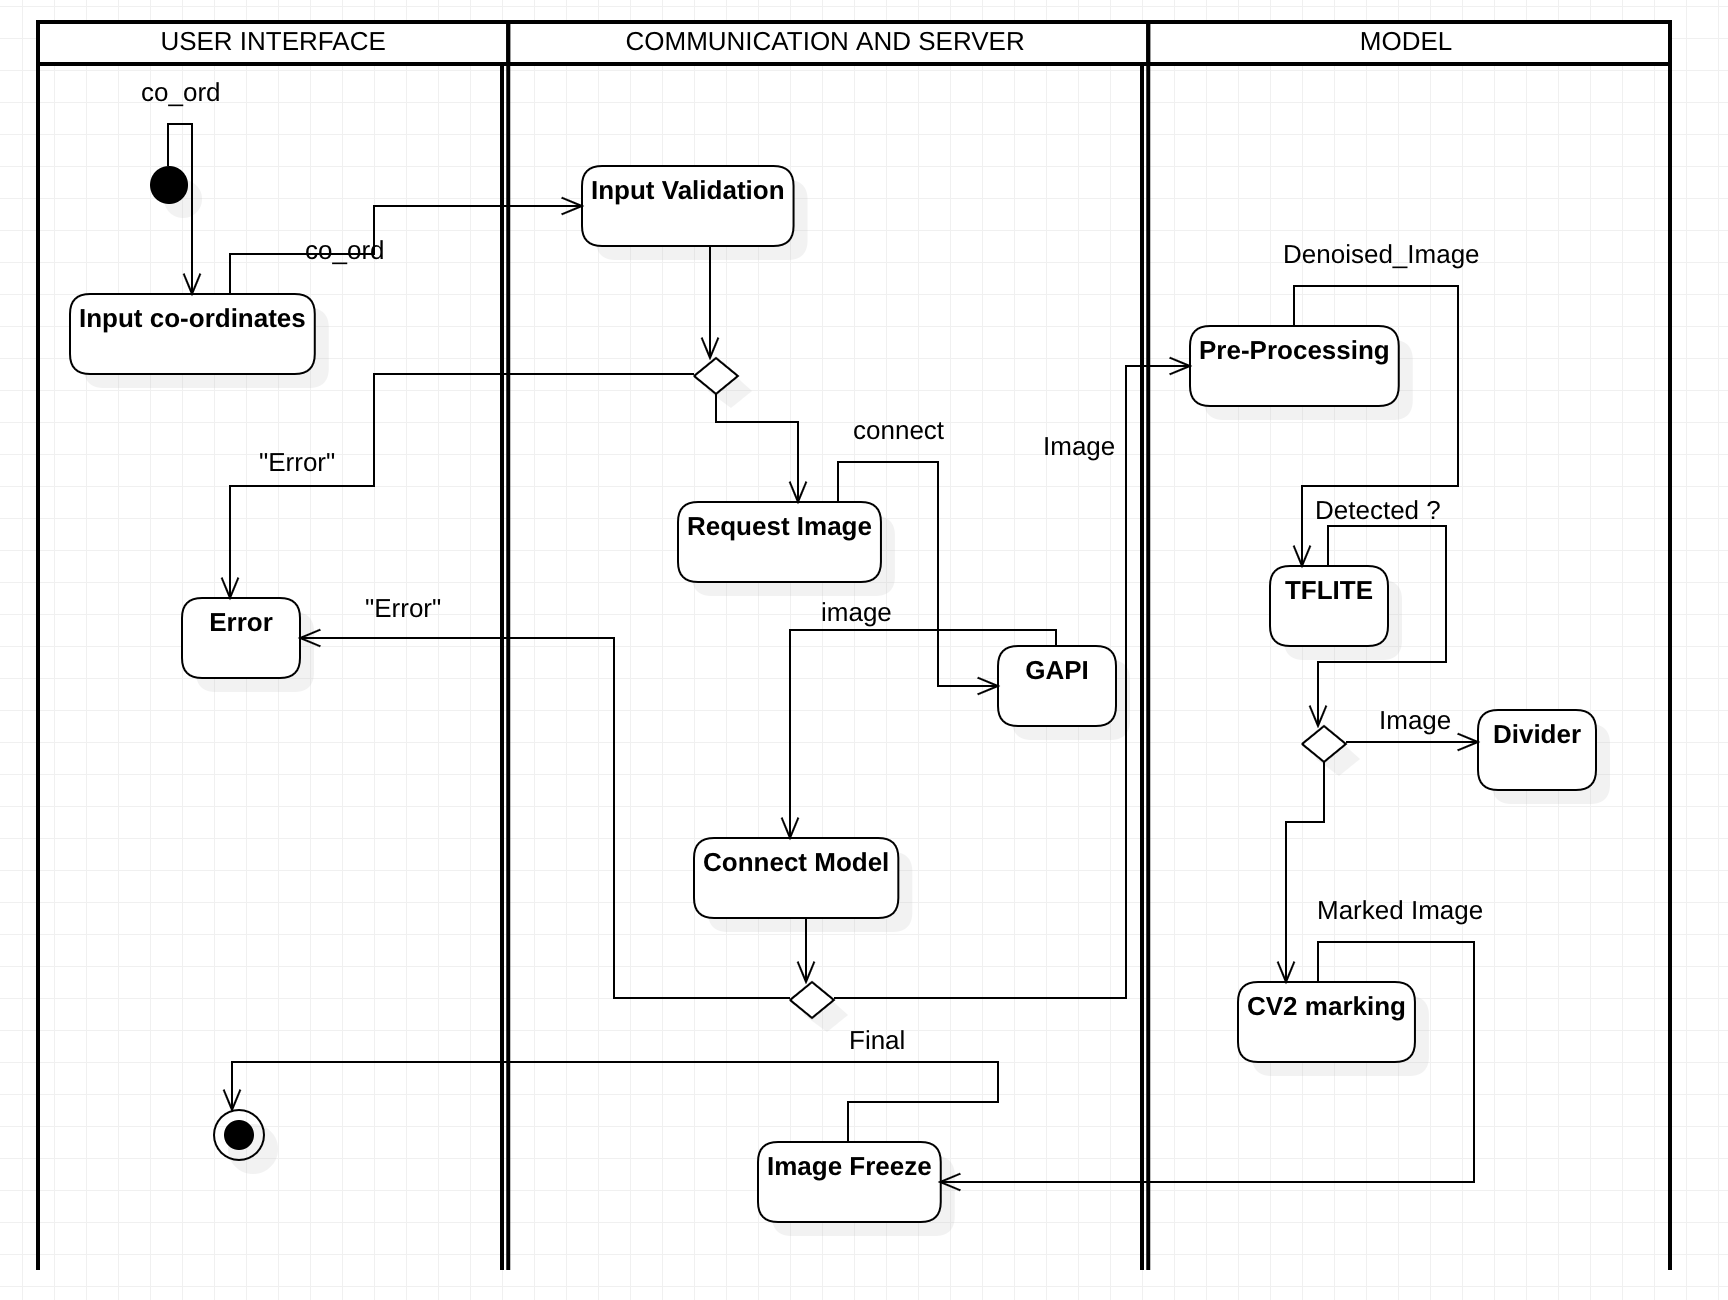
\includegraphics[scale=0.6]{images/activity.png}
\section{Component Diagram}
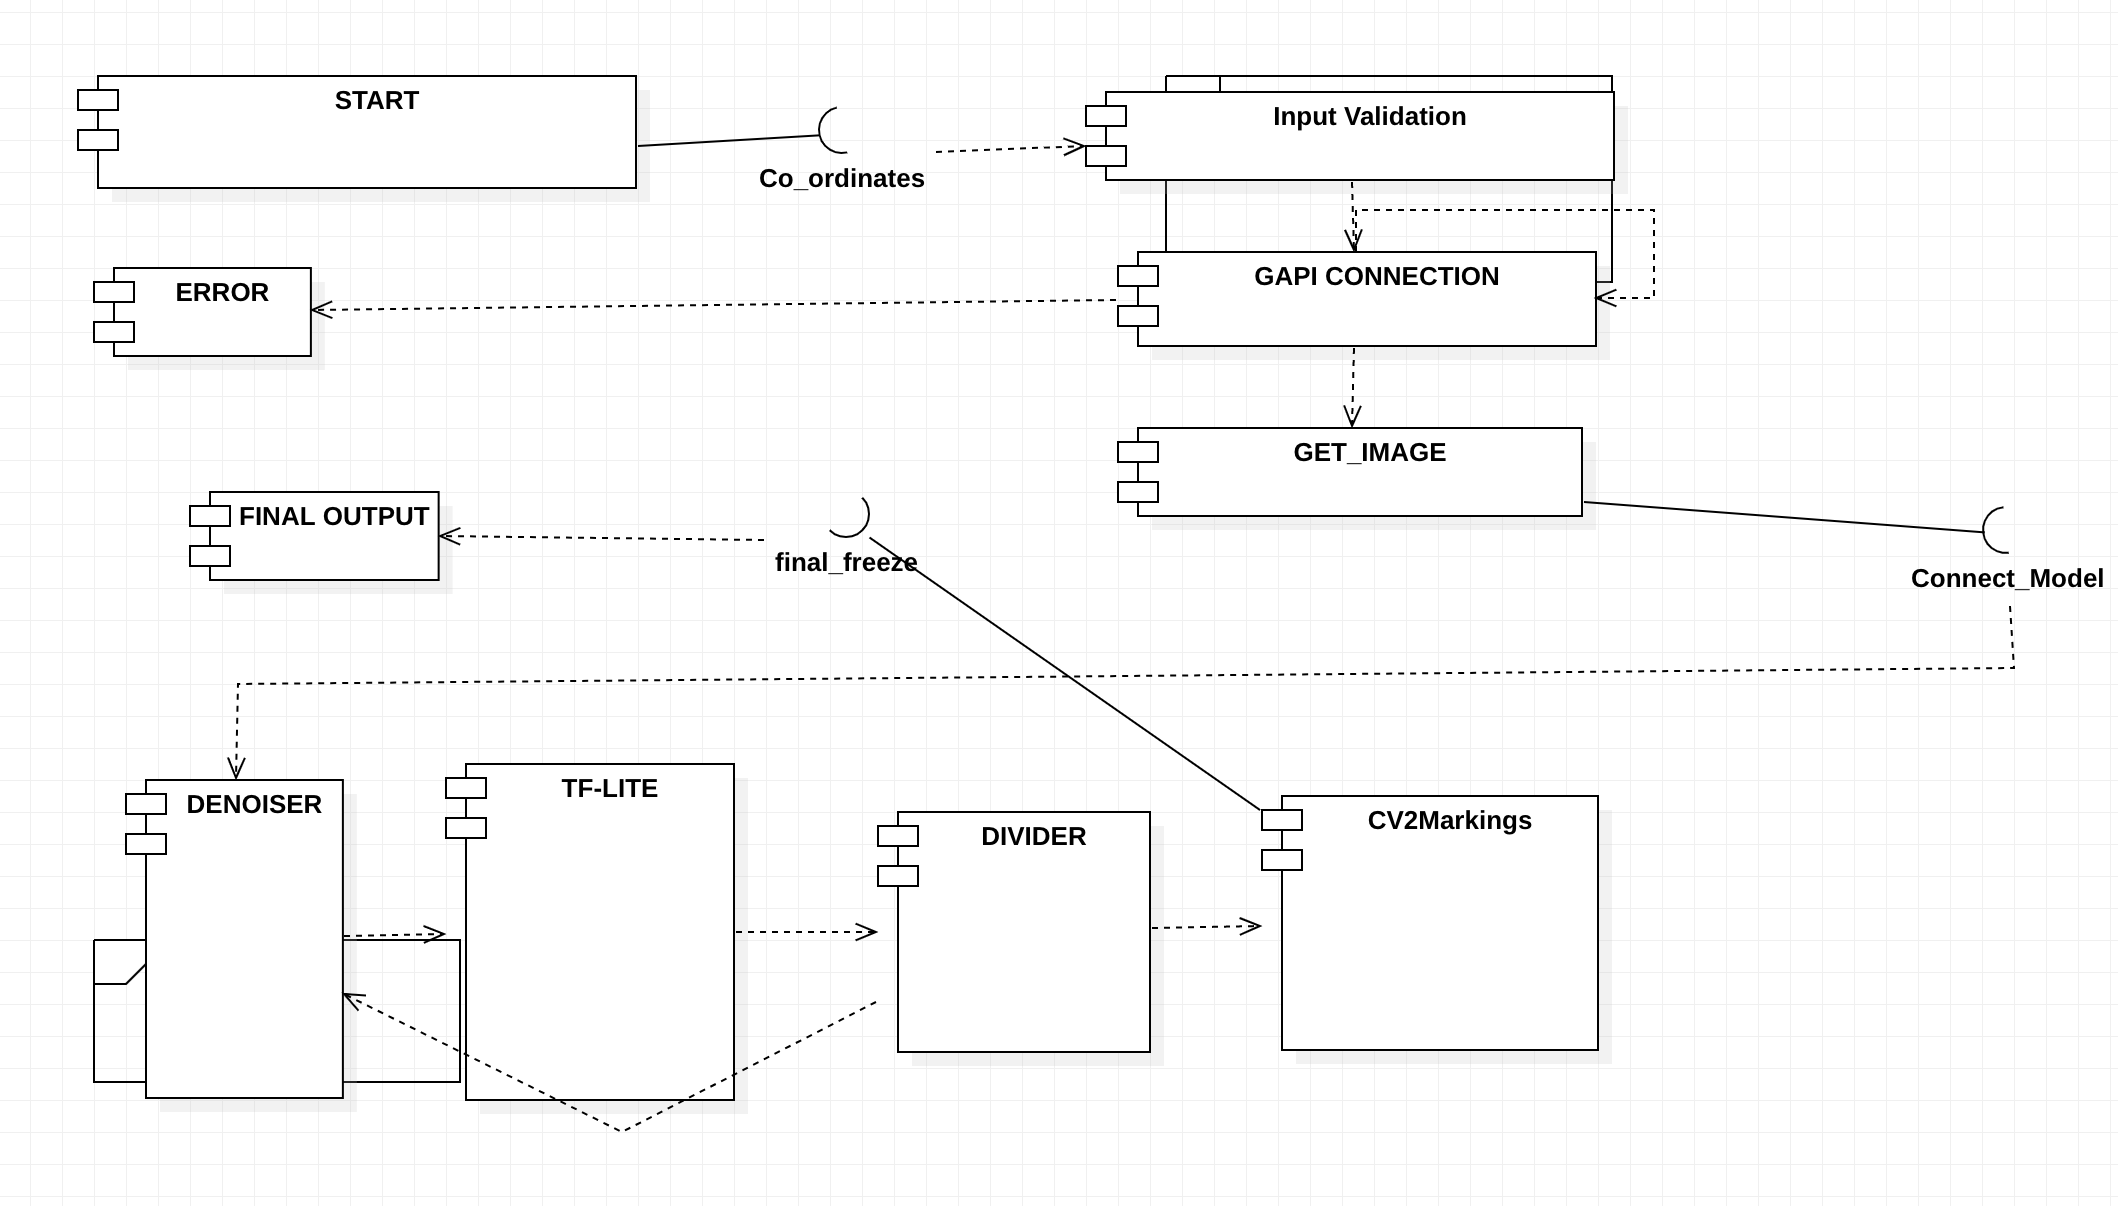
\includegraphics[scale=0.4]{images/comp.png}
\section{Package Diagram}
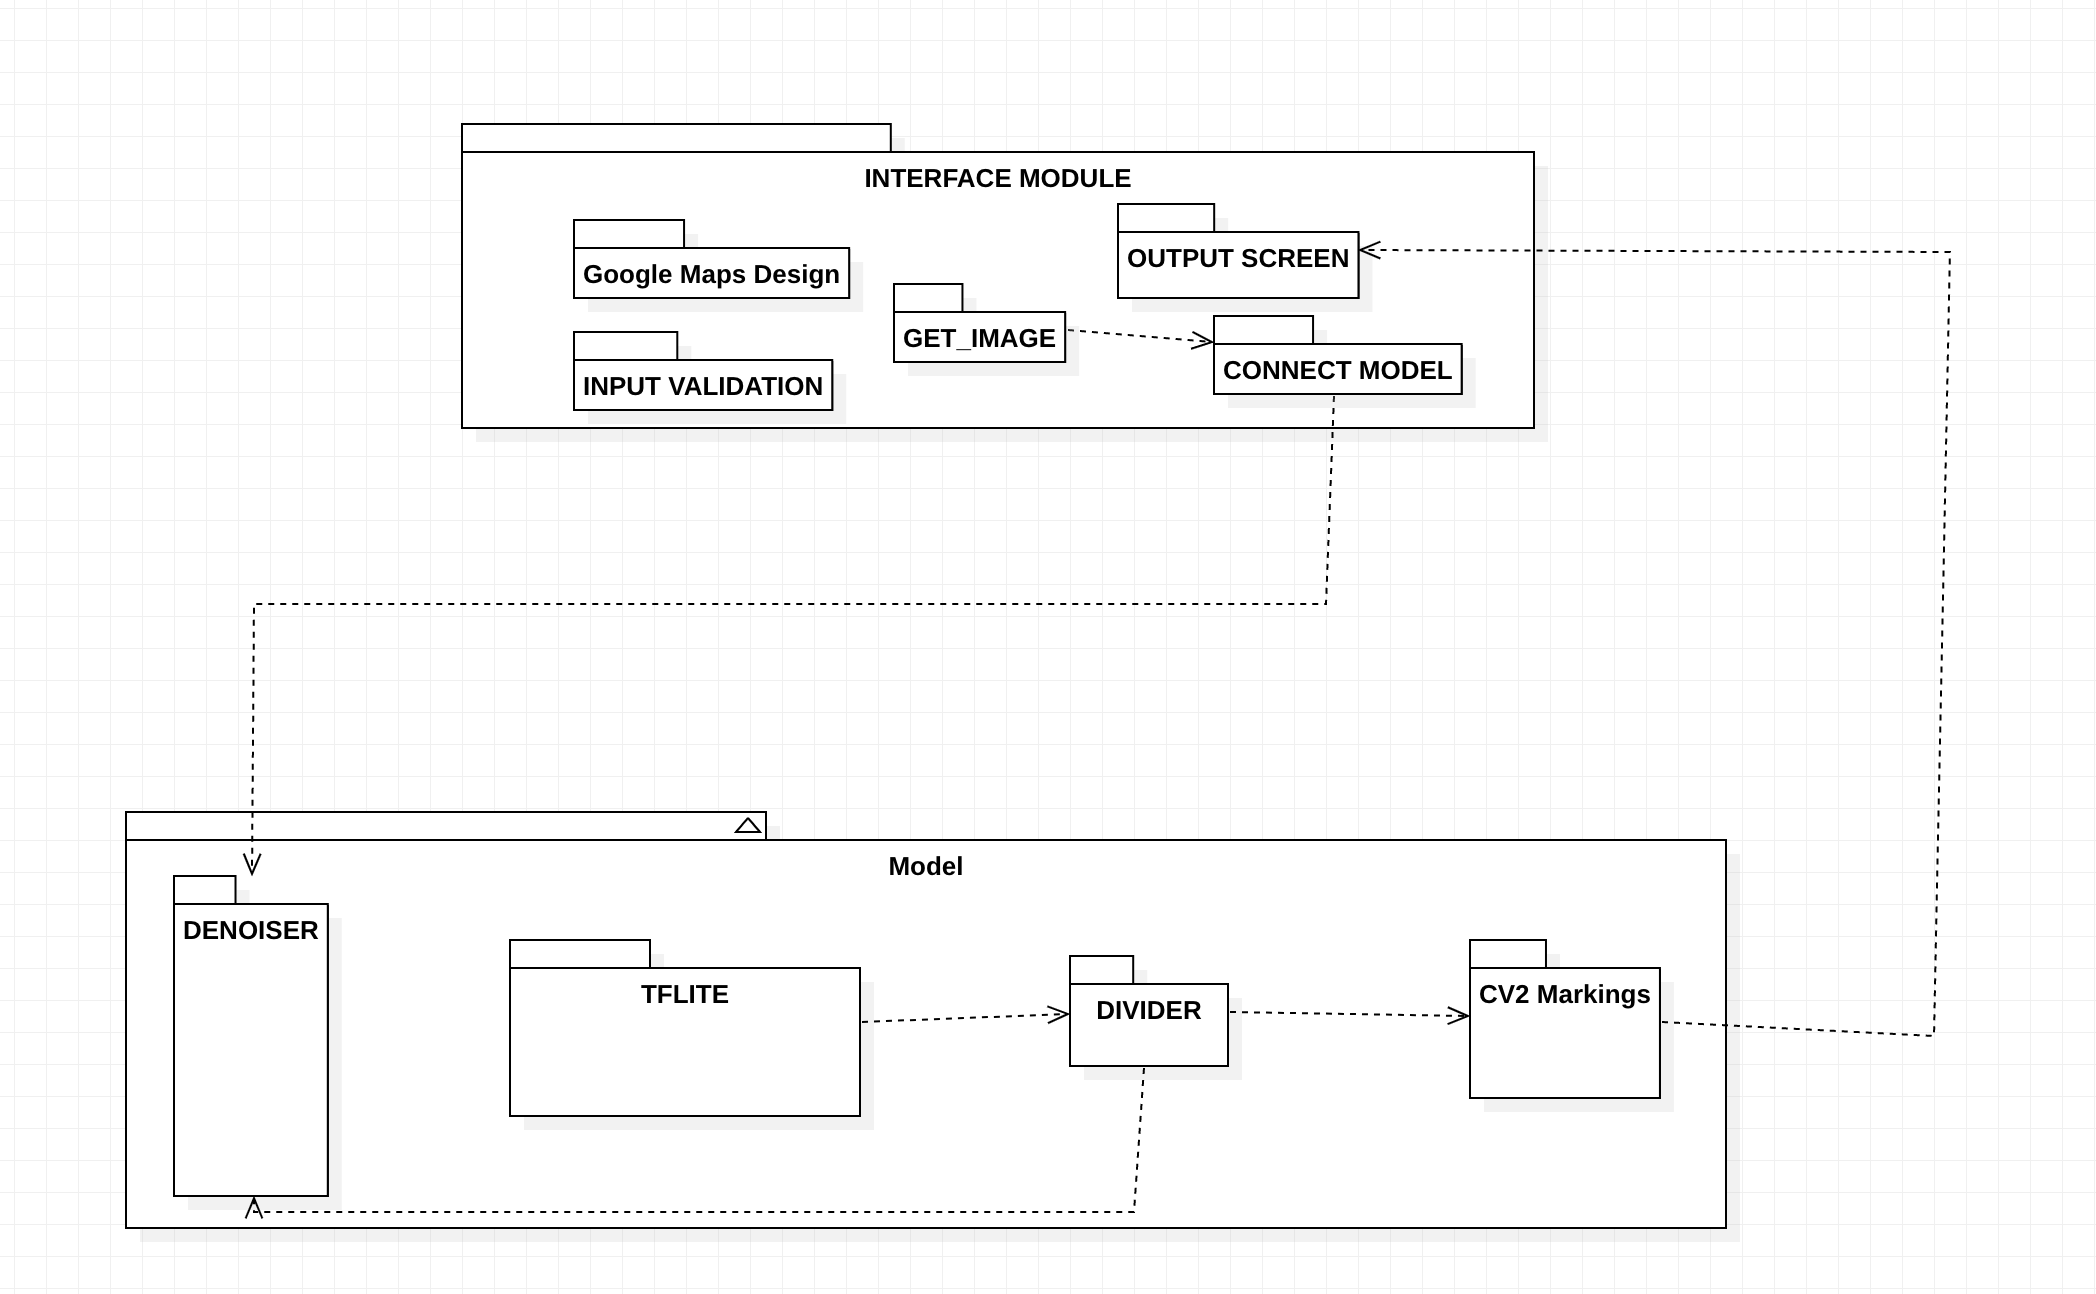
\includegraphics[scale=0.4]{images/package.png}
\section{Deployment Diagram}
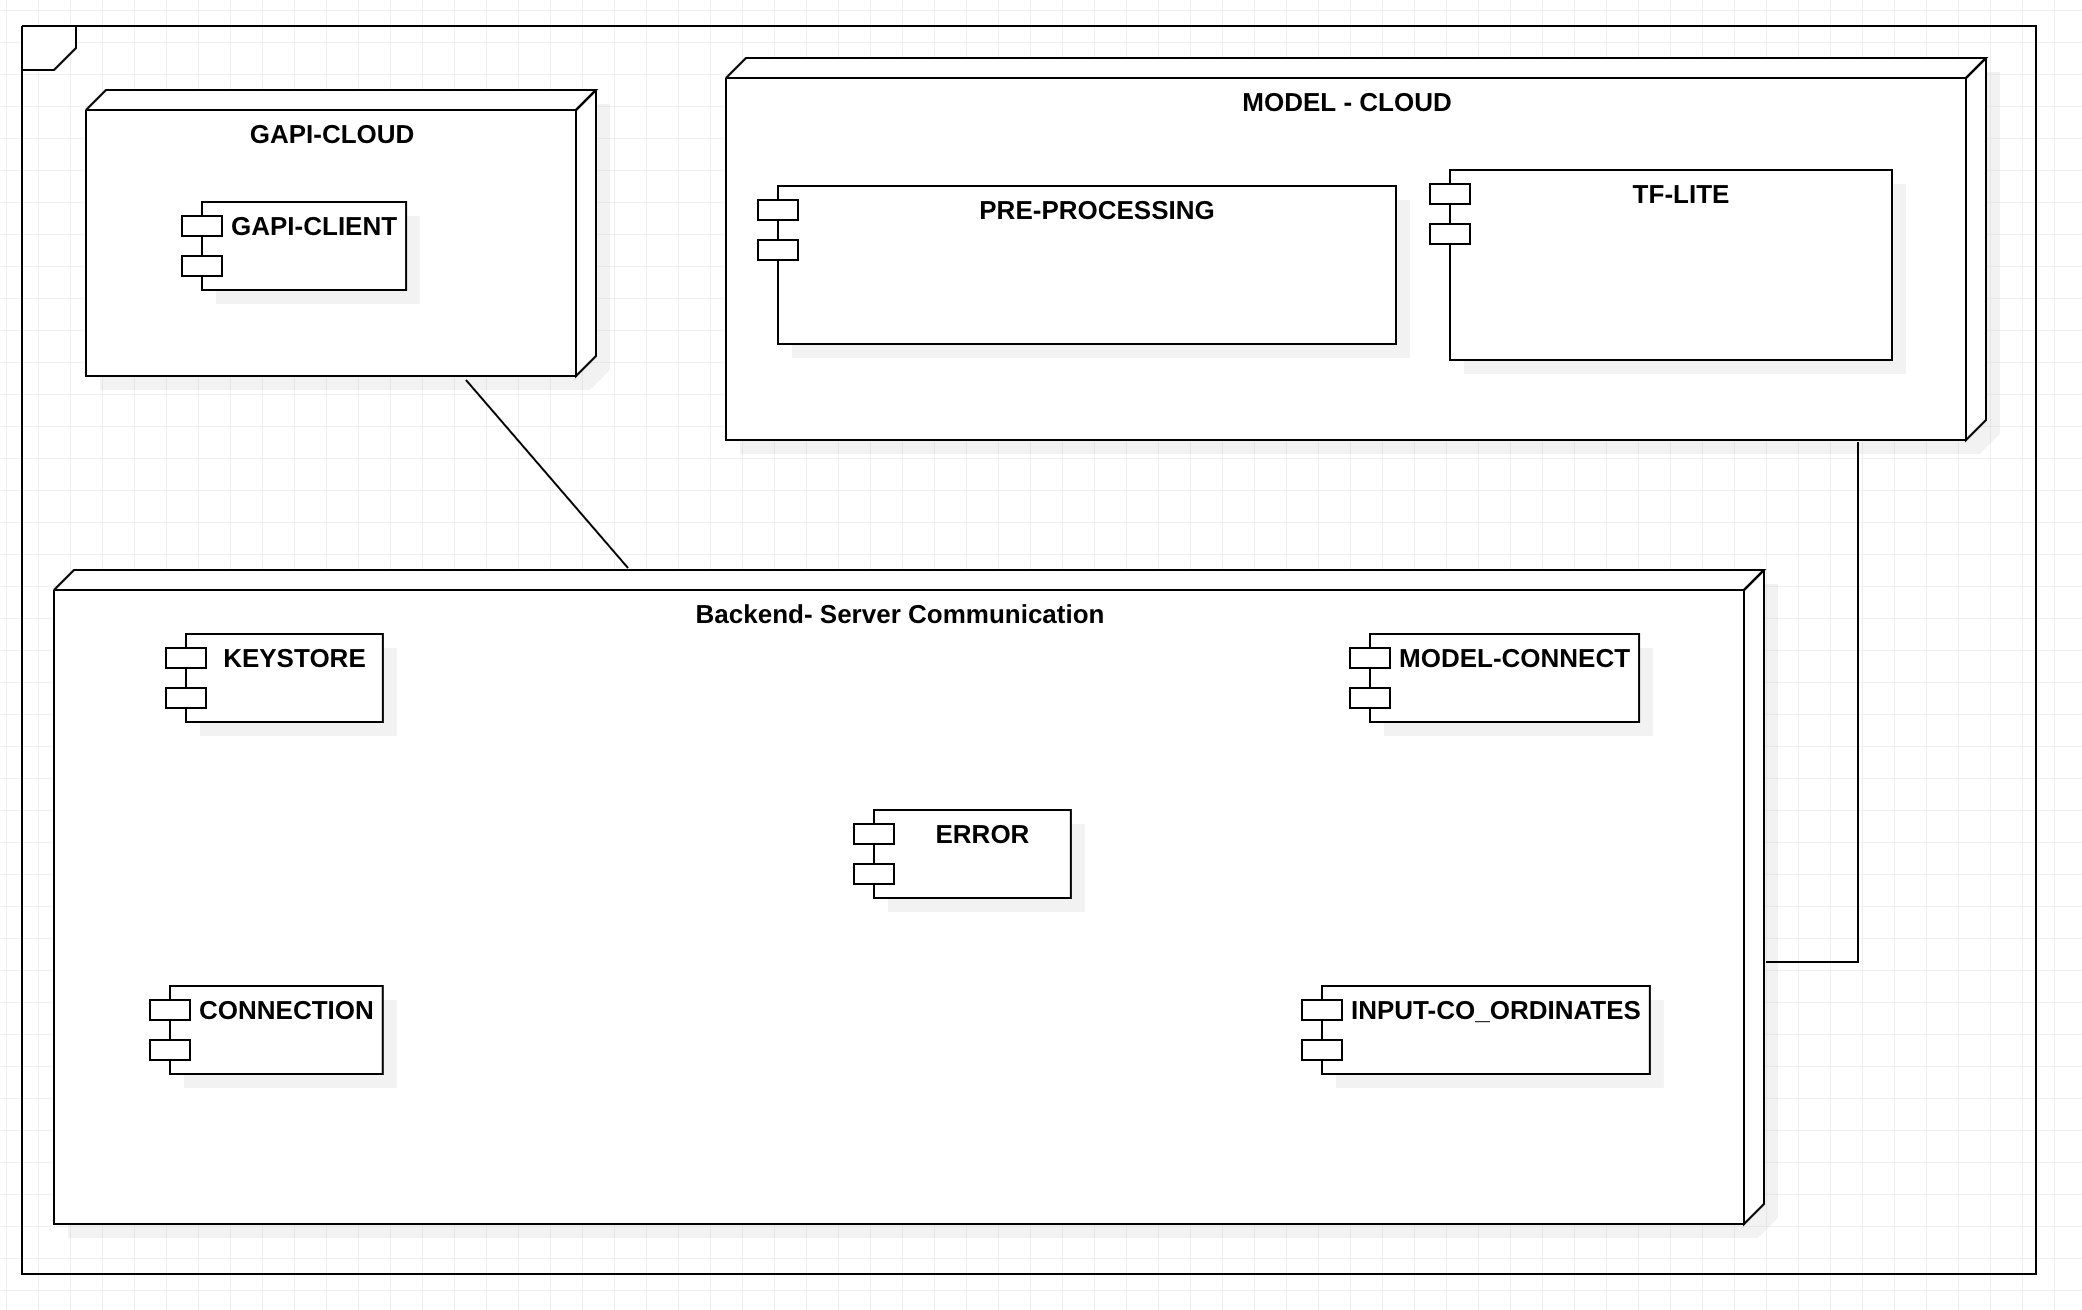
\includegraphics[scale=0.4]{images/deploy.png}

\chapter{Implementation}

\section{Google Cloud Platform (GCP)}
\subsection{GCP Dashboard}
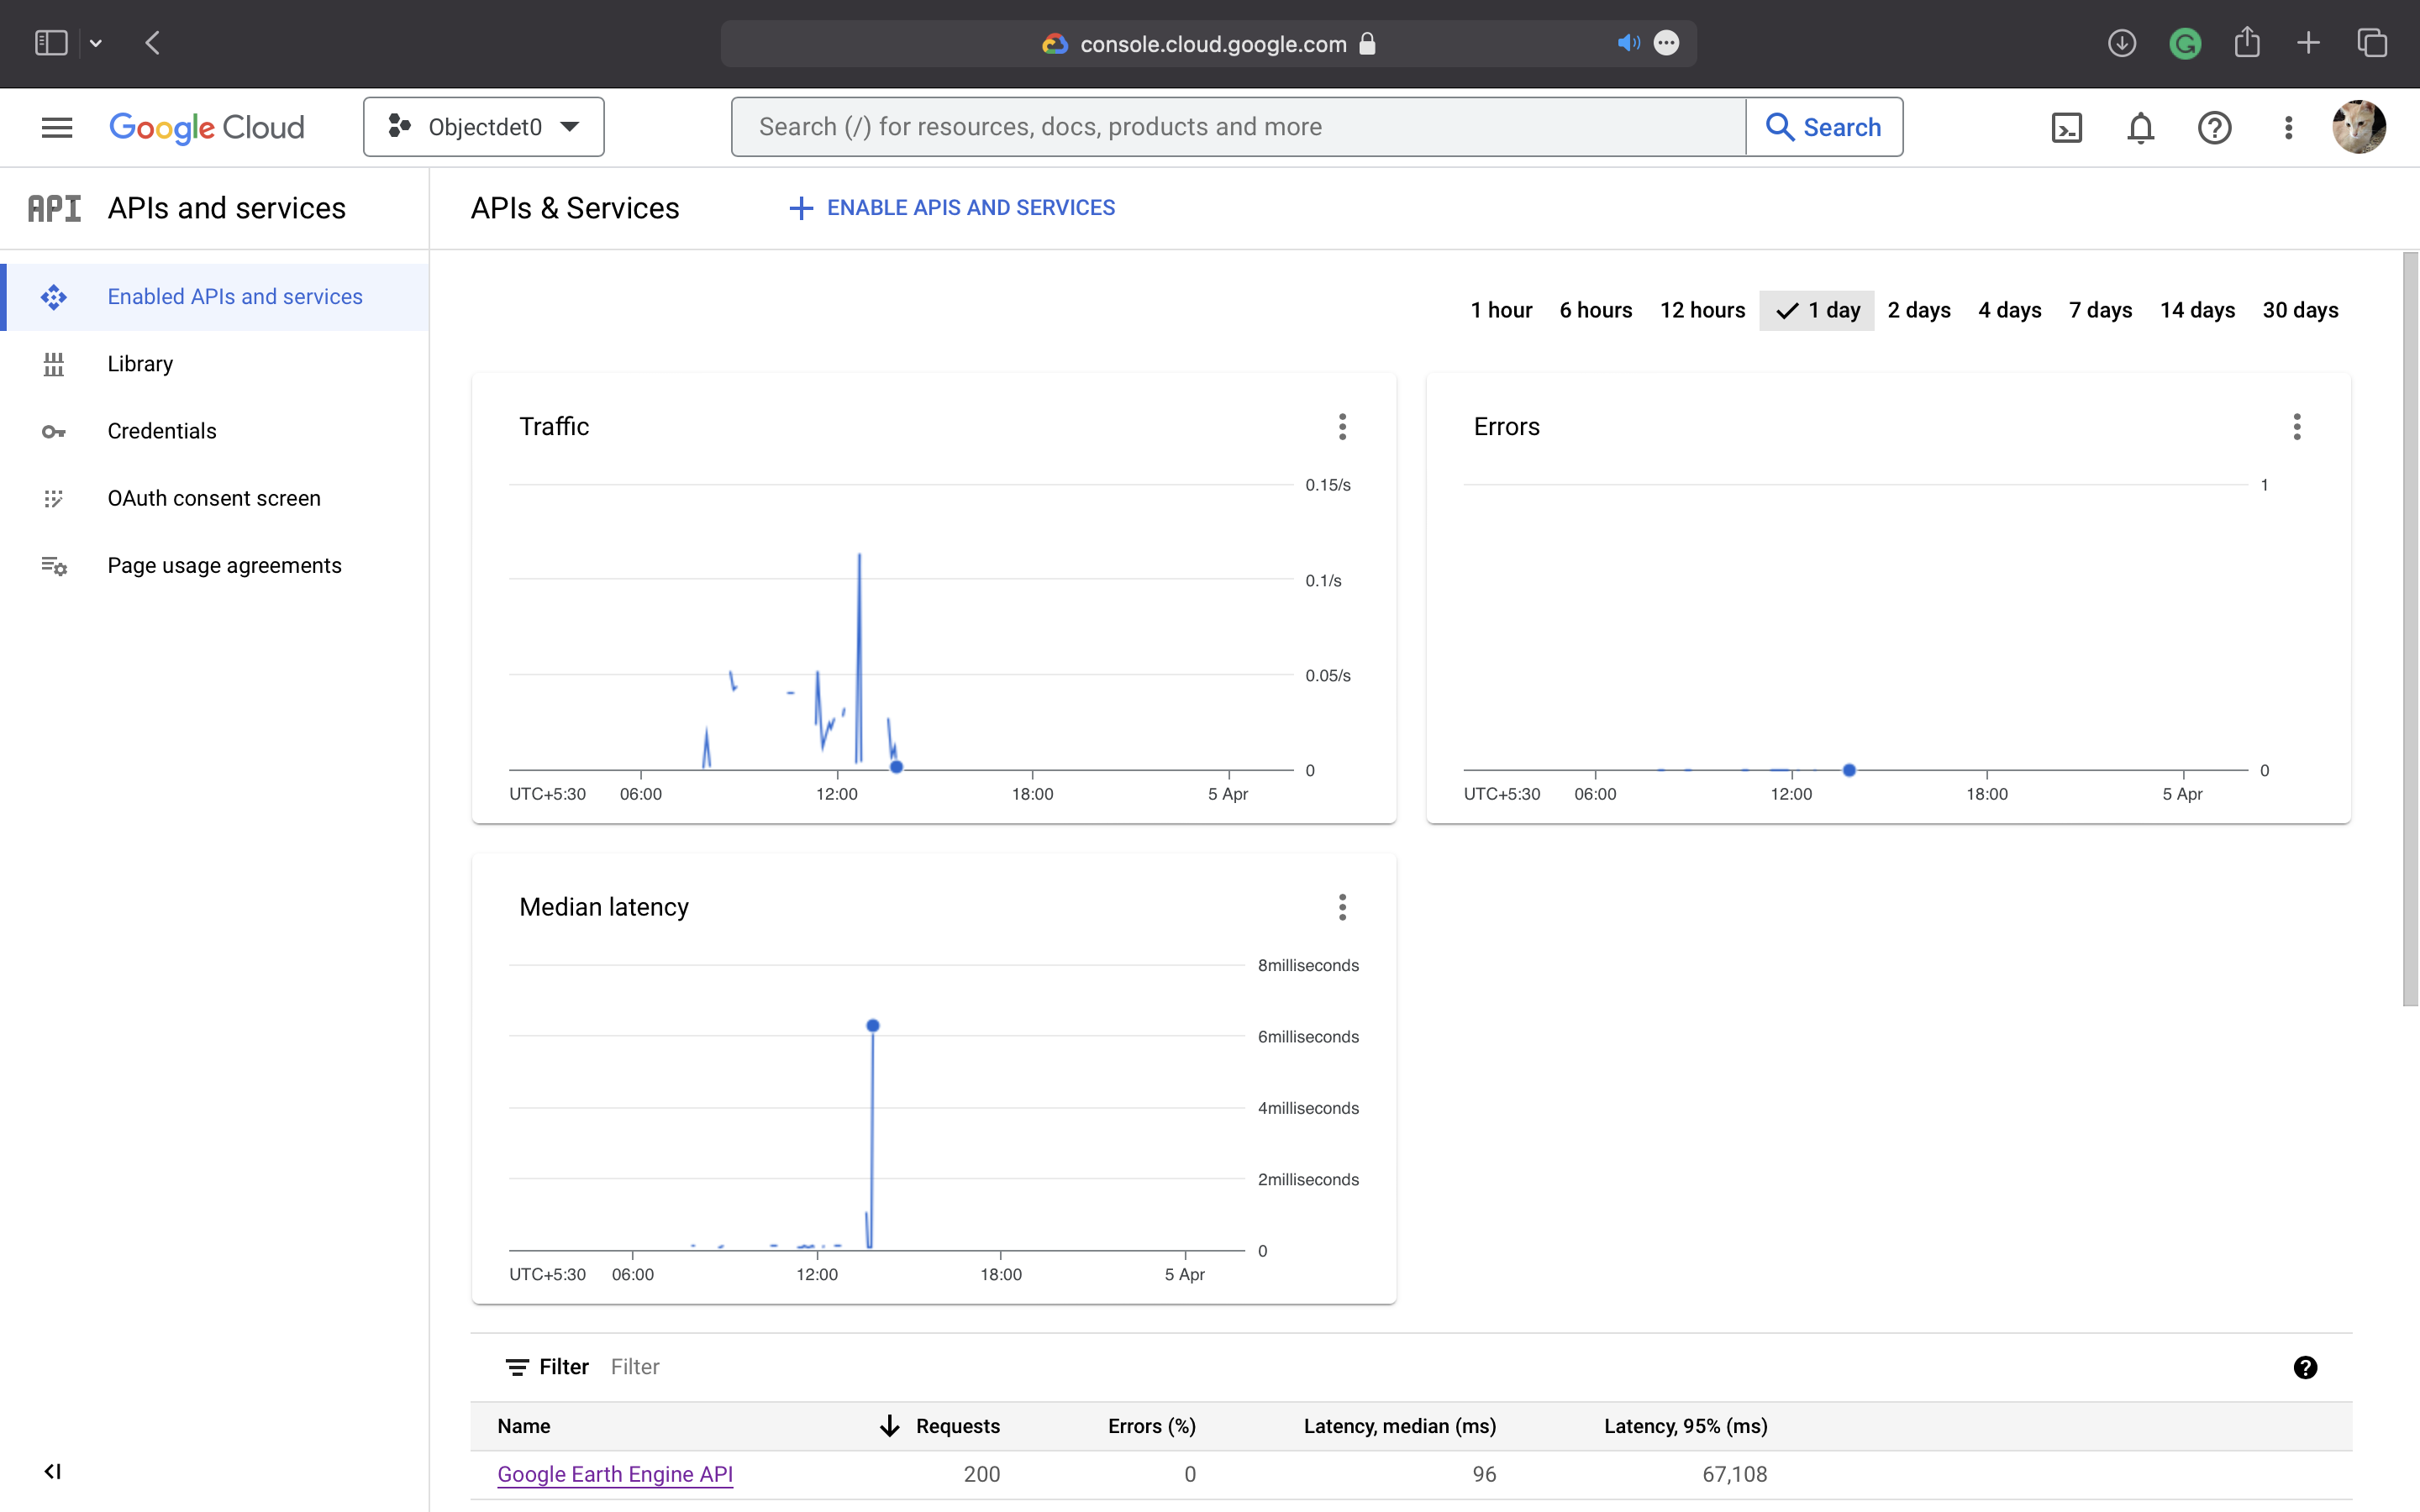
\includegraphics[scale=0.34]{screenshts/1.png}
\subsection{GCP Service Accounts}
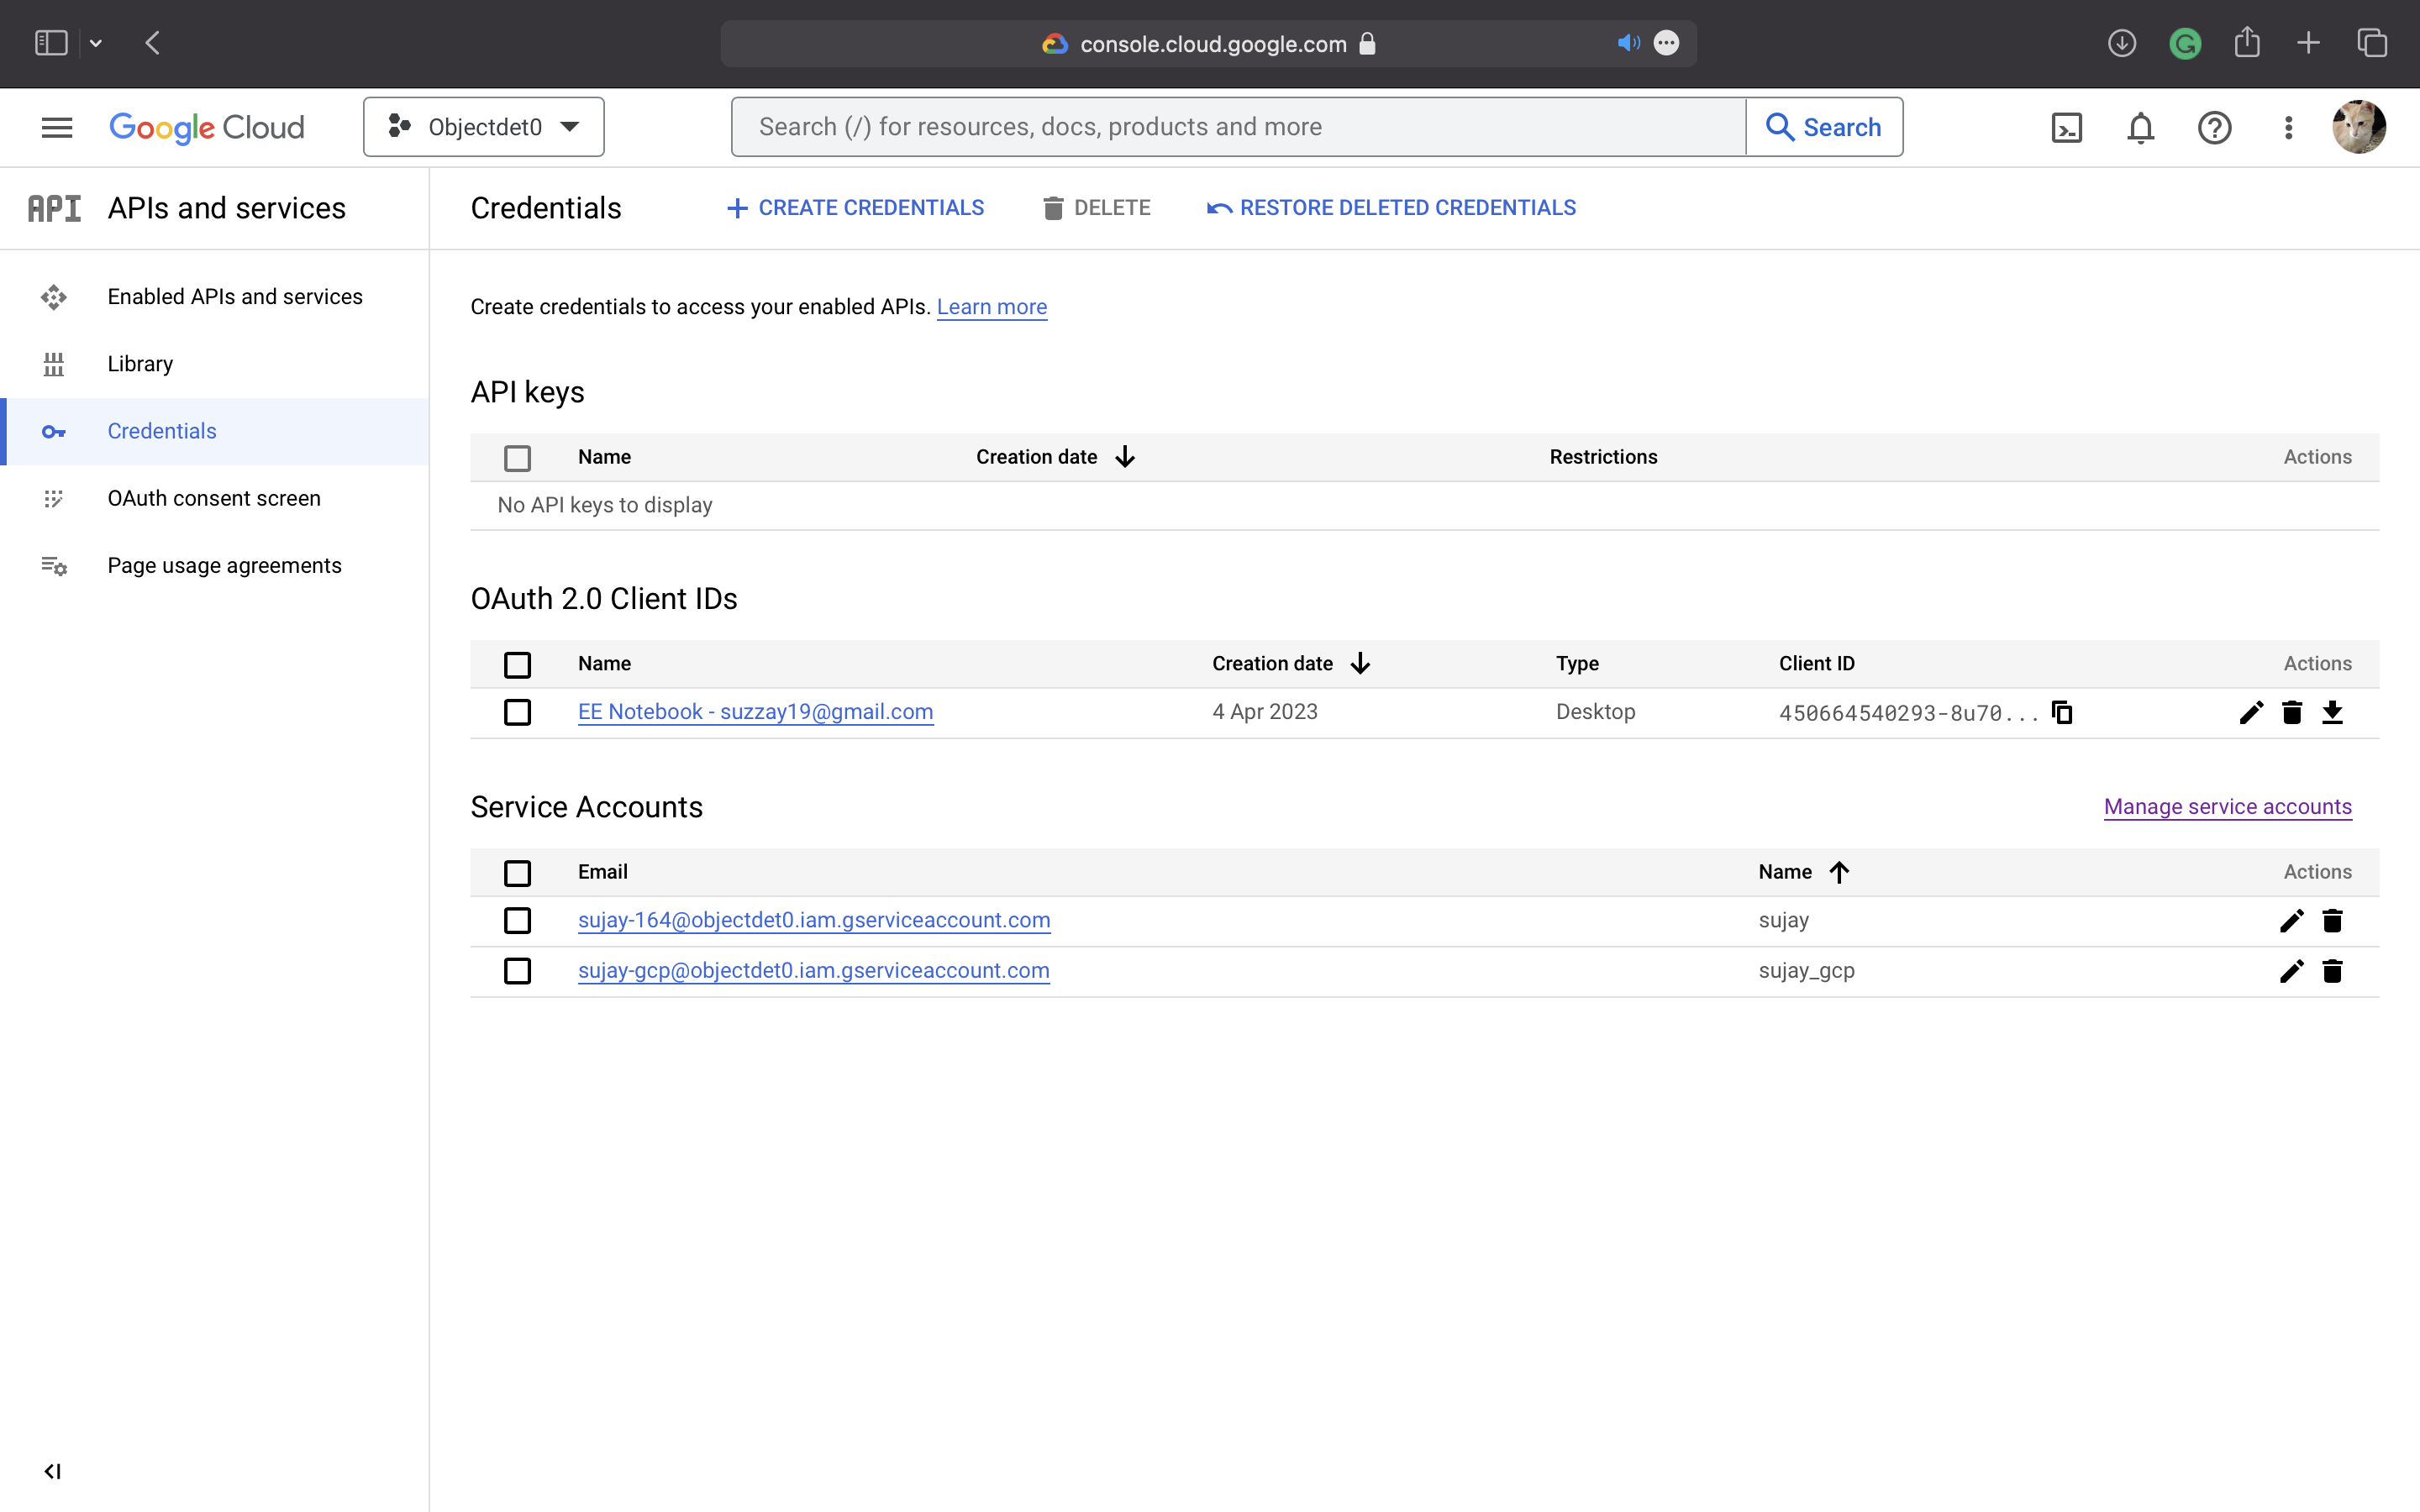
\includegraphics[scale=0.3]{screenshts/2.png}
\subsection{GCP Identity and Access Management}
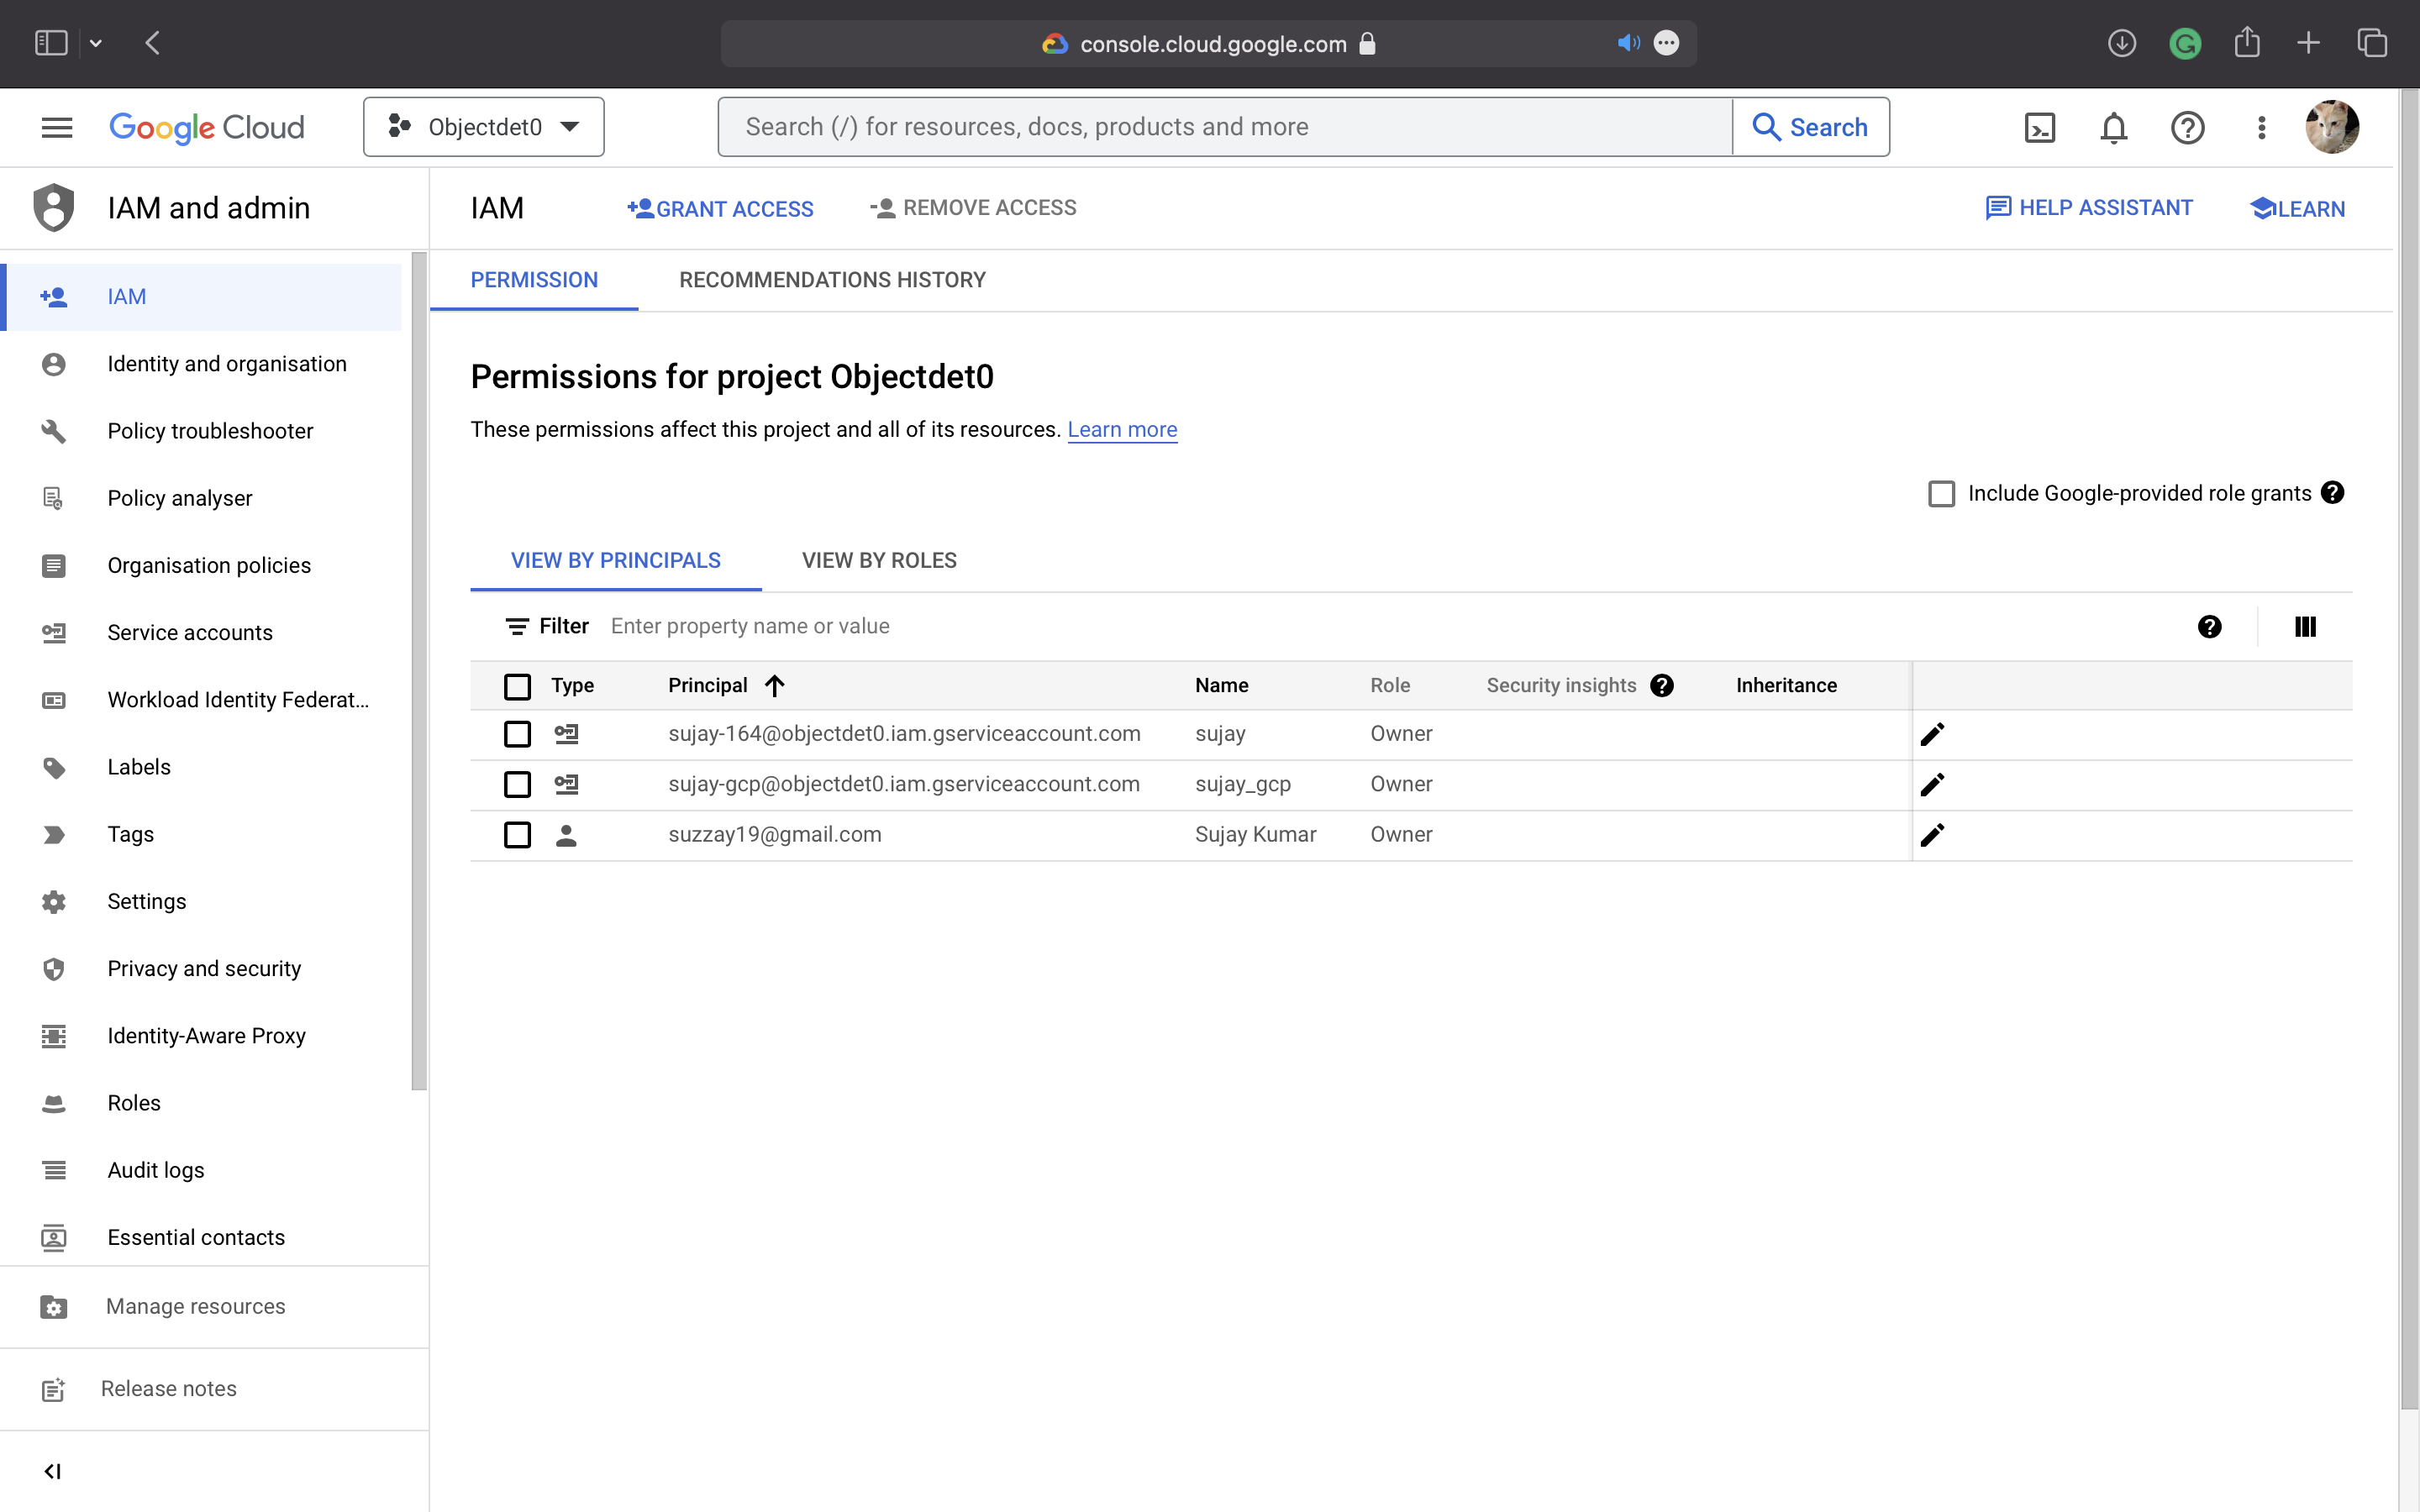
\includegraphics[scale=0.3]{screenshts/3.png}

\section{Data Analysis and Data Visualization}
\begin{lstlisting}[language=JavaScript]
// Determine 10-year mean LSTs

/**** Start of imports. If edited, may not auto-convert in the playground. ****/
var VisPar = {"opacity":1,"bands":["constant"],"min":-5,"max":40,"palette":["002bff","00ff36","fbff00","ff0000"]};
/***** End of imports. If edited, may not auto-convert in the playground. *****/
//variables
var numyears=10; //number of years
var firstyear=2005; //first year (beast after 2002)

//function oneyear mean
var oneyearmean=function(MYD,MOD){
var MYDm = MYD.mean();
var MODm = MOD.mean();
var LST_do=MODm.expression( //im transfering to celcius here so I don't have to worry about different band names
  '(0.02*LST - 273.15)',{
    'LST' : MODm.select('LST_Day_1km')
  });
var LST_no=MODm.expression(
  '(0.02*LST - 273.15)',{
    'LST' : MODm.select('LST_Night_1km')
  });
var LST_dy=MYDm.expression(
  '(0.02*LST - 273.15)',{
    'LST' : MYDm.select('LST_Day_1km')
  });
var LST_ny=MYDm.expression(
  '(0.02*LST - 273.15)',{
    'LST' : MYDm.select('LST_Night_1km')
  });
var LST = ee.ImageCollection([LST_dy,LST_ny,LST_do,LST_no]).mean();
//going with image collection to get the mean, couse than i don't have to fiure out how to work with the 'no value' pixels
  return LST;
};

//function 10 year mean month
var meanmonth=function(from,to,month){
var LST2=ee.List([]); //dummy to fill with LSTs

for (var year = firstyear; year < firstyear+numyears; year++) {
var quarter_from = ee.Date(year.toString() +from);
var quarter_to = ee.Date(year.toString() +to);
if (month == 12) {
  var yy=year+1;
    quarter_to = ee.Date(yy.toString() +to);
}
var MYD = ee.ImageCollection('MODIS/MYD11A1')
  .filterDate(quarter_from, quarter_to);
var MOD = ee.ImageCollection('MODIS/MOD11A1')
  .filterDate(quarter_from, quarter_to);
  LST=oneyearmean(MYD,MOD);
  LST2=LST2.add(LST);
}
var LST3=ee.ImageCollection(LST2);
return LST3.mean();
};

//start main code
var LST= ee.Image.constant(0); //dummy to fill with LSTs
for (var month=1;month<13;month++){
   var m =month+1;
  var daypermonth=31;
  if (month == 2){
    daypermonth=28;
  } else if  (month == 4 | month == 6 | month == 9 | month == 11) {
    daypermonth=30;
  }
  var from=('-'+month.toString()+'-01');
  var to=('-'+m.toString()+'-01'); 
  if (month == 12) {
    var to=('-01-01');
} 
    LST=LST.add(meanmonth(from,to,month).multiply(ee.Image.constant(daypermonth)));
}
//print('LST',LST);
LST=LST.expression(
  '(LST/365)',{
    'LST' : LST
  }); 
Map.setCenter(0, 0, 1); 
Map.addLayer(LST,VisPar,'LST');
 Export.image(LST, 'LST', {
  scale: 1000,
  maxPixels: 1e10
}); 
\end{lstlisting}
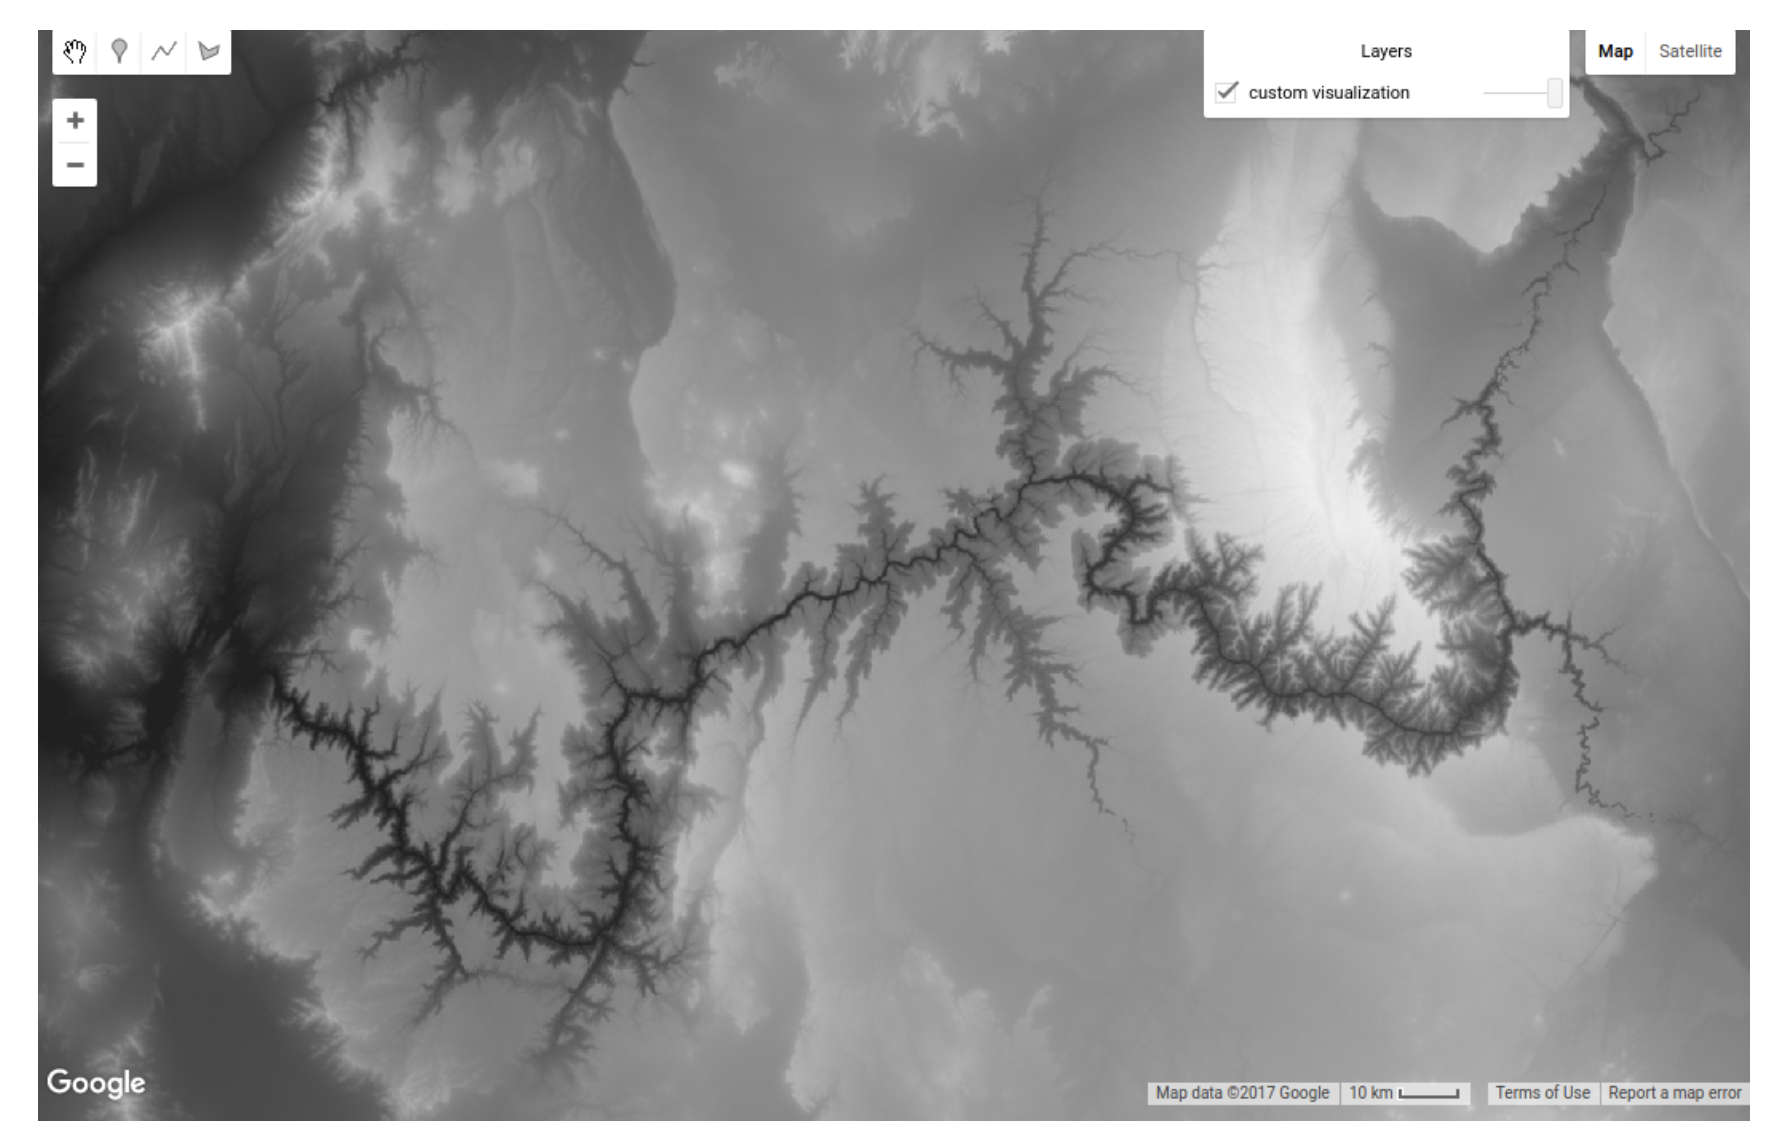
\includegraphics[scale=0.6]{screenshts/4.png}

\section{Pre-Procesing Using Patchify}
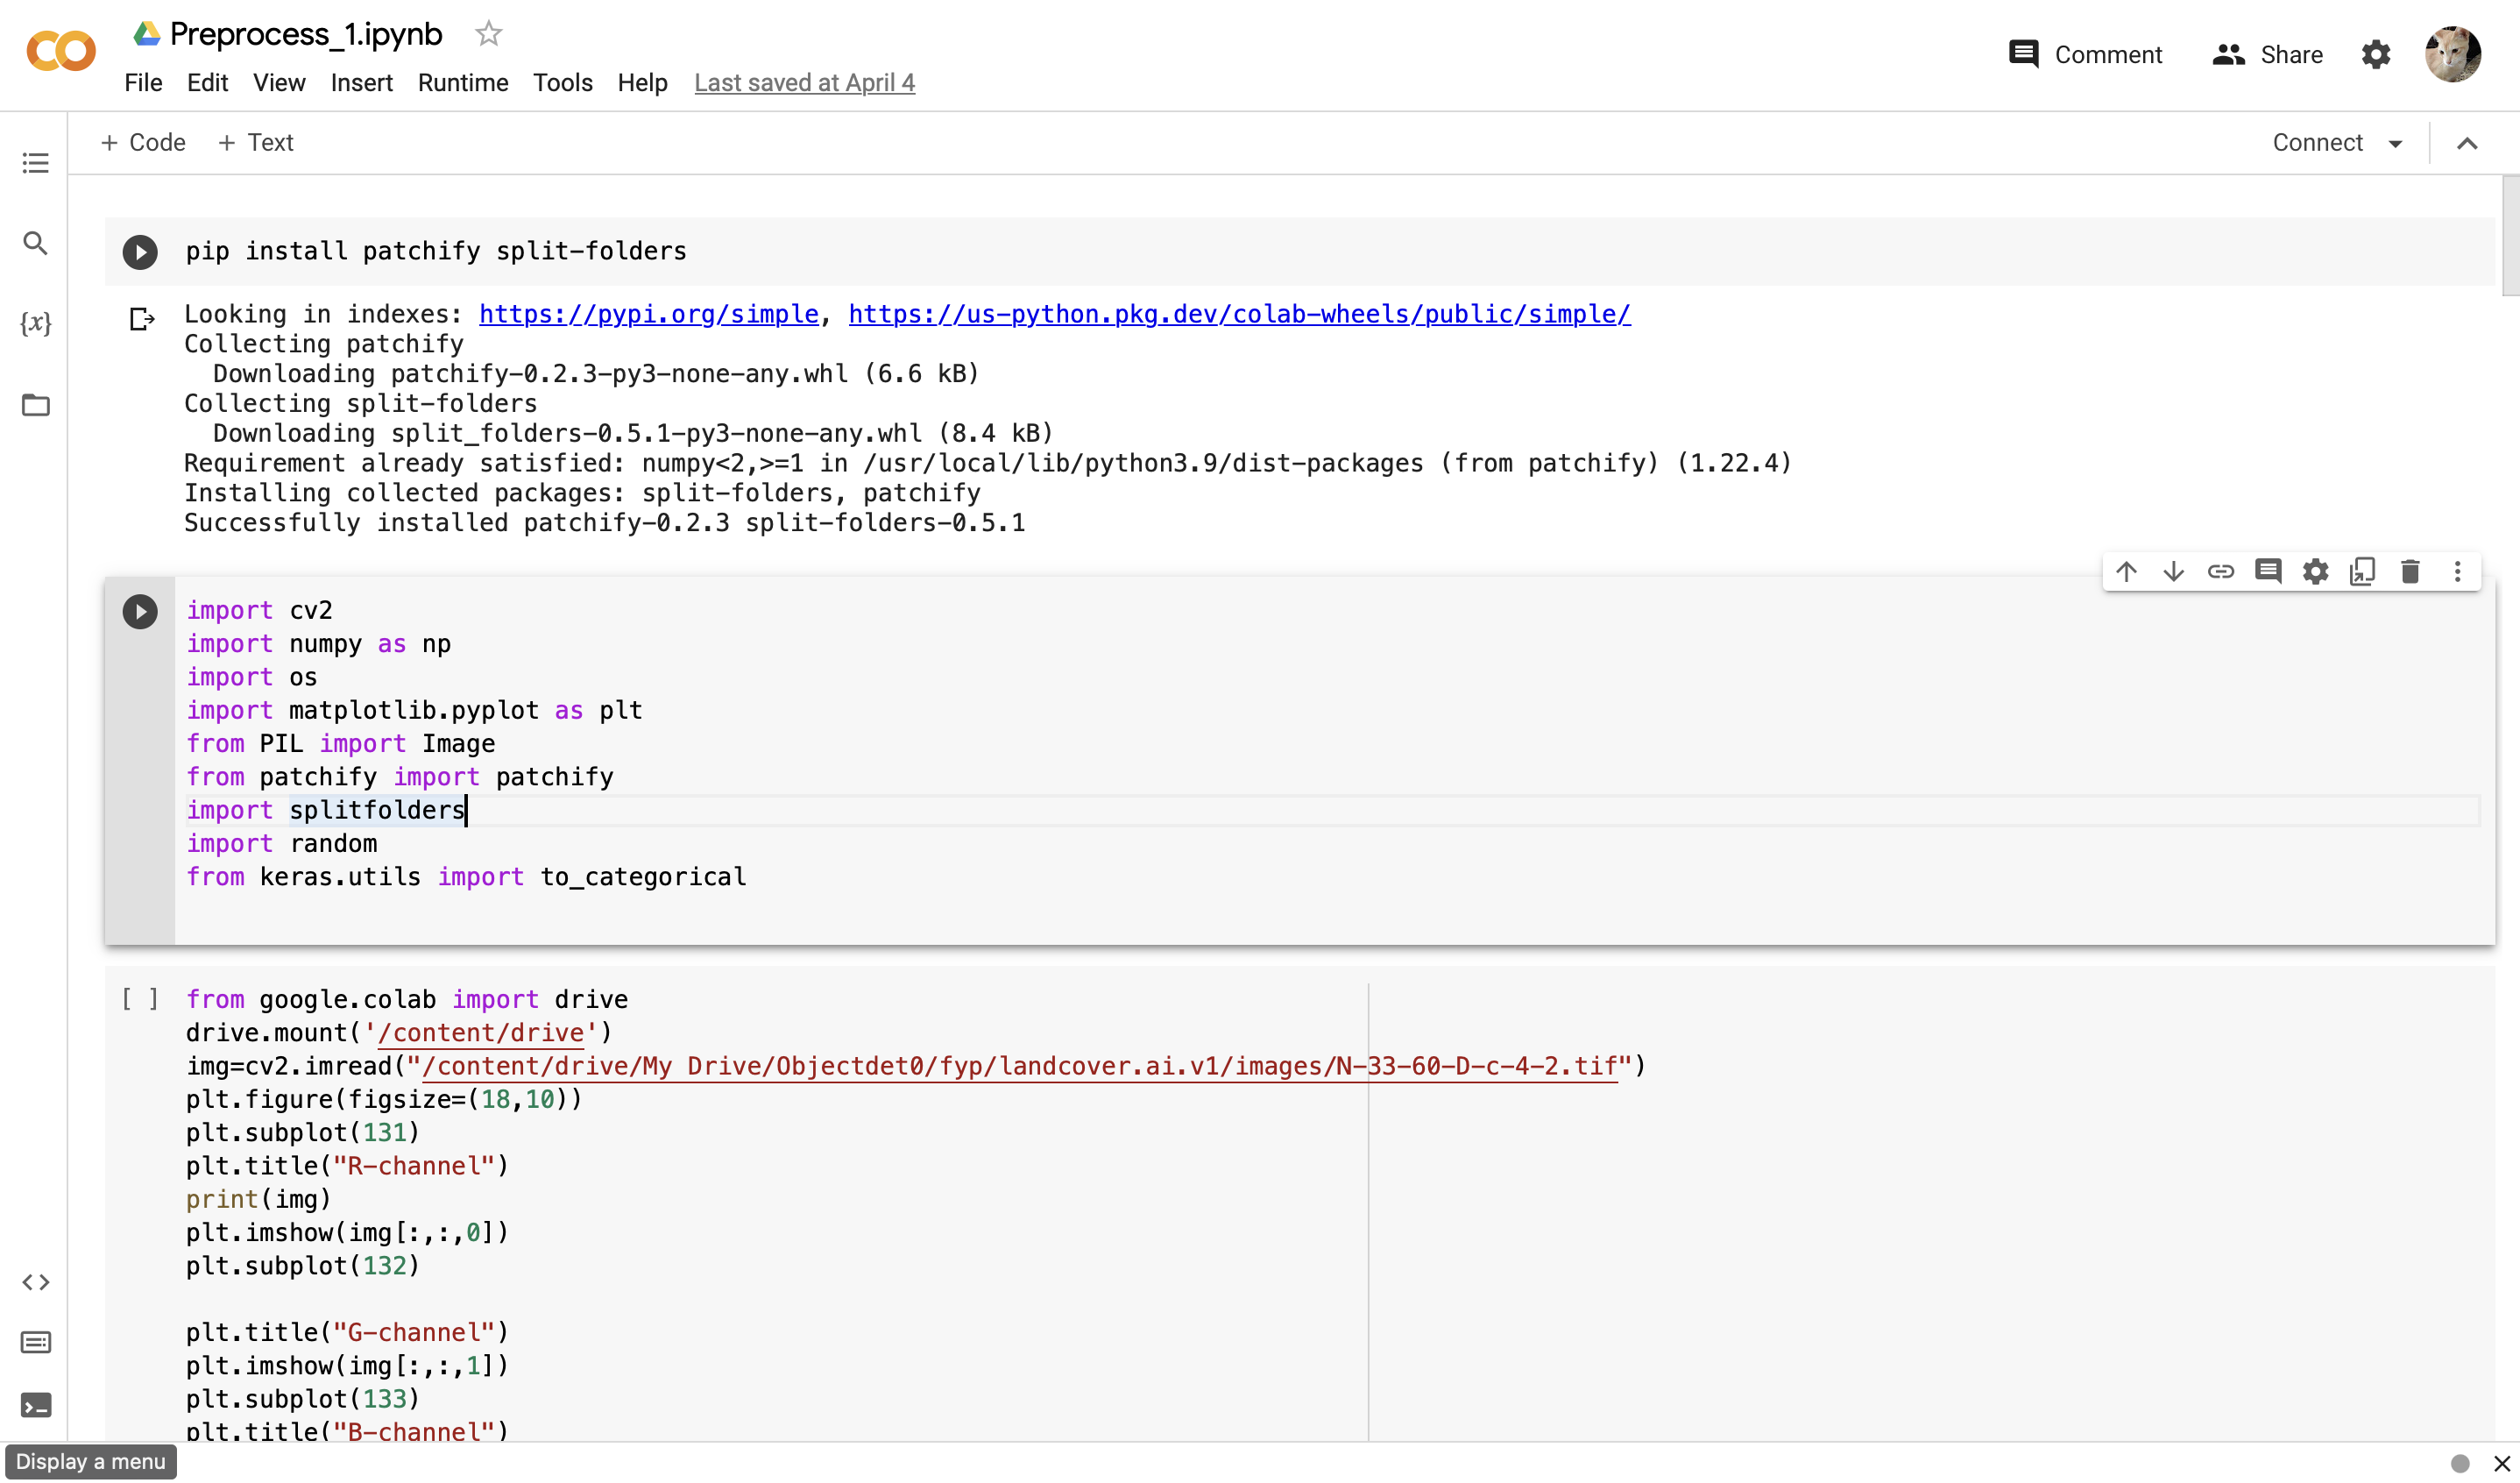
\includegraphics[scale=0.4]{screenshts/5.png}
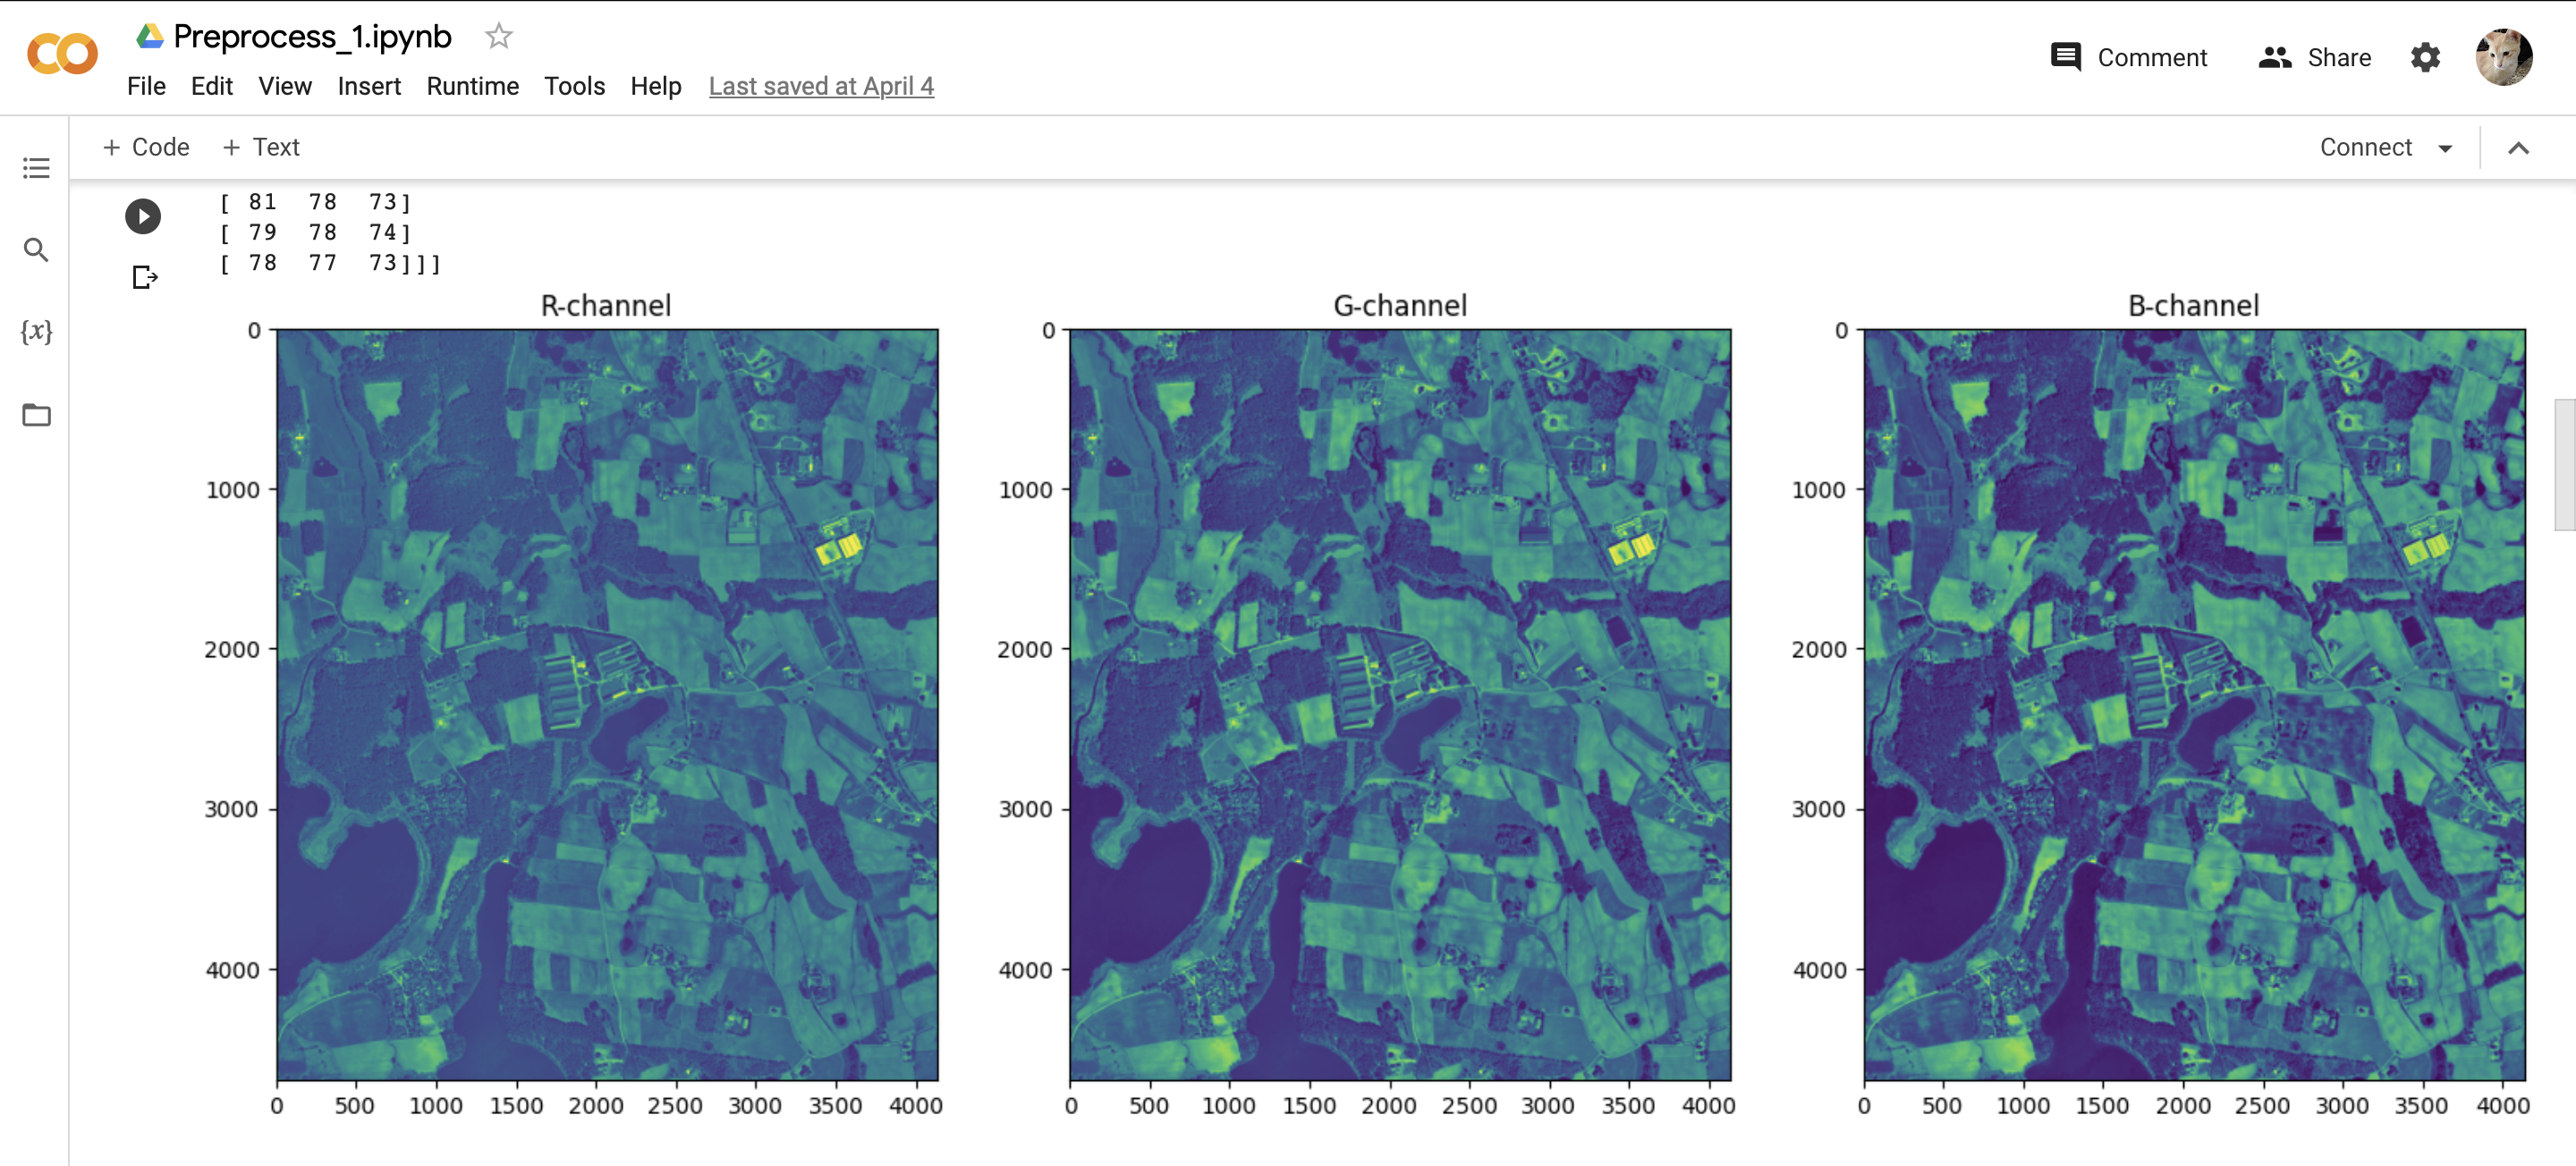
\includegraphics[scale=0.4]{screenshts/6.png}
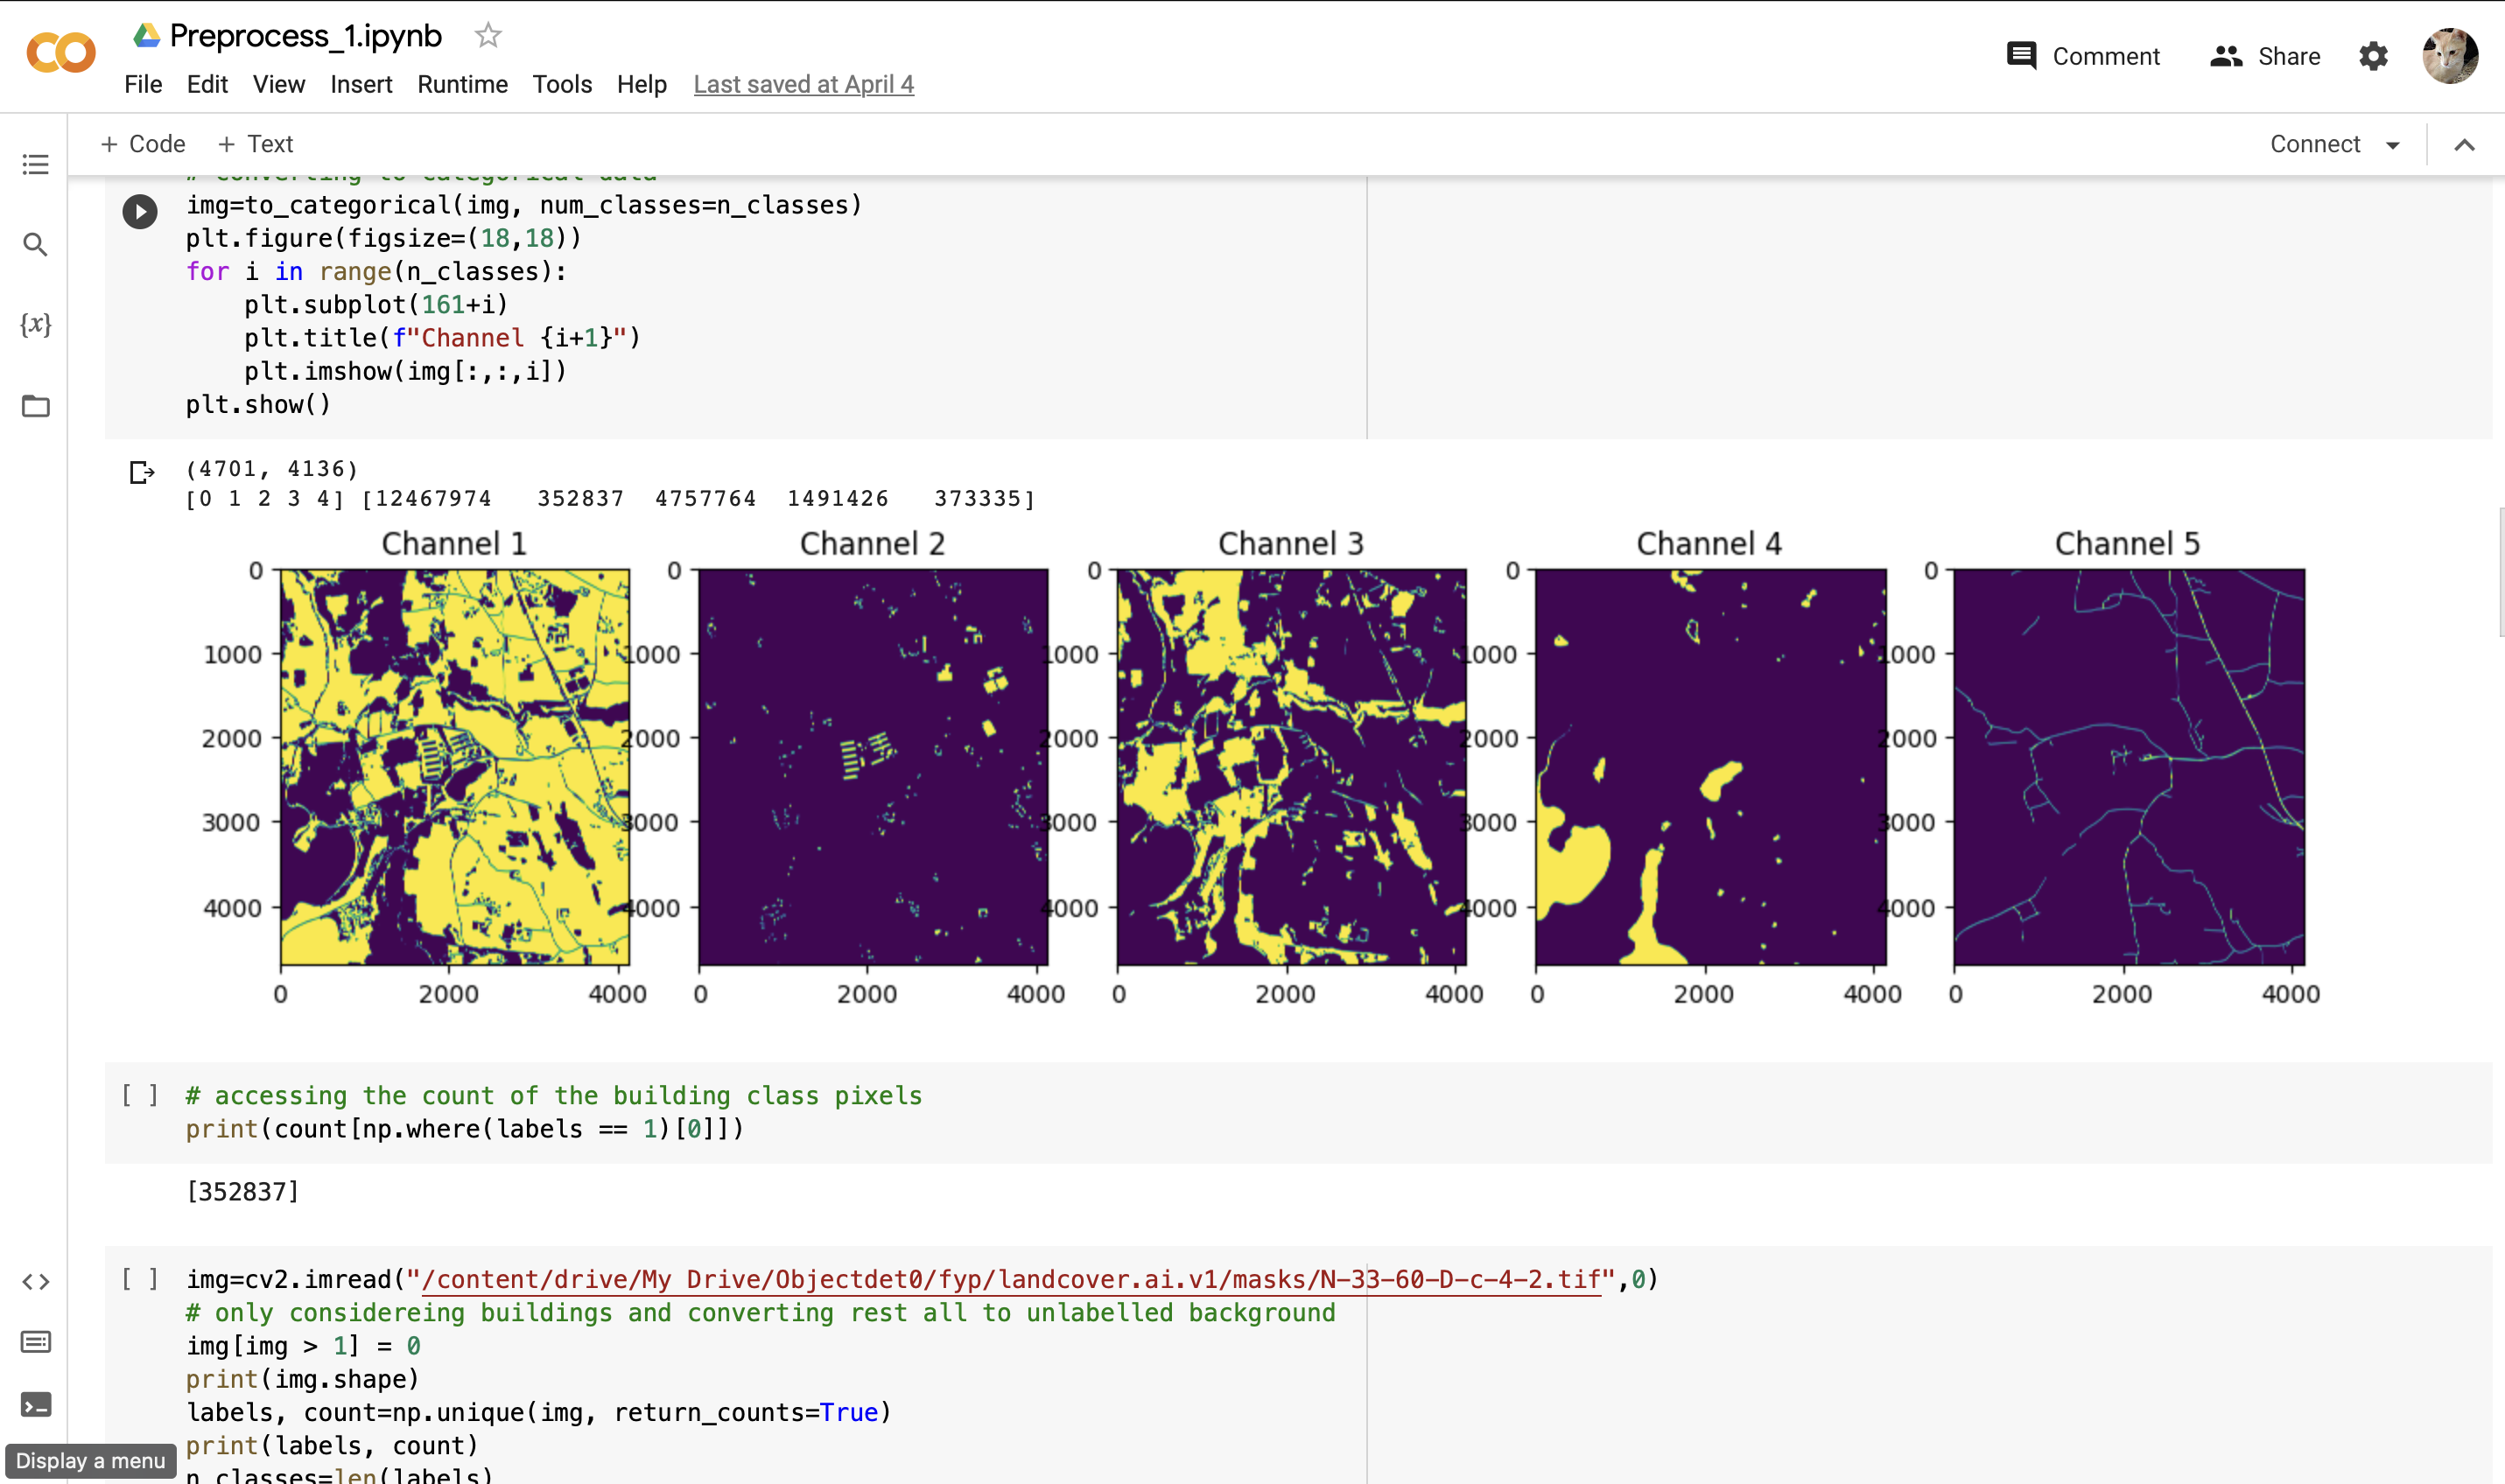
\includegraphics[scale=0.34]{screenshts/7.png}
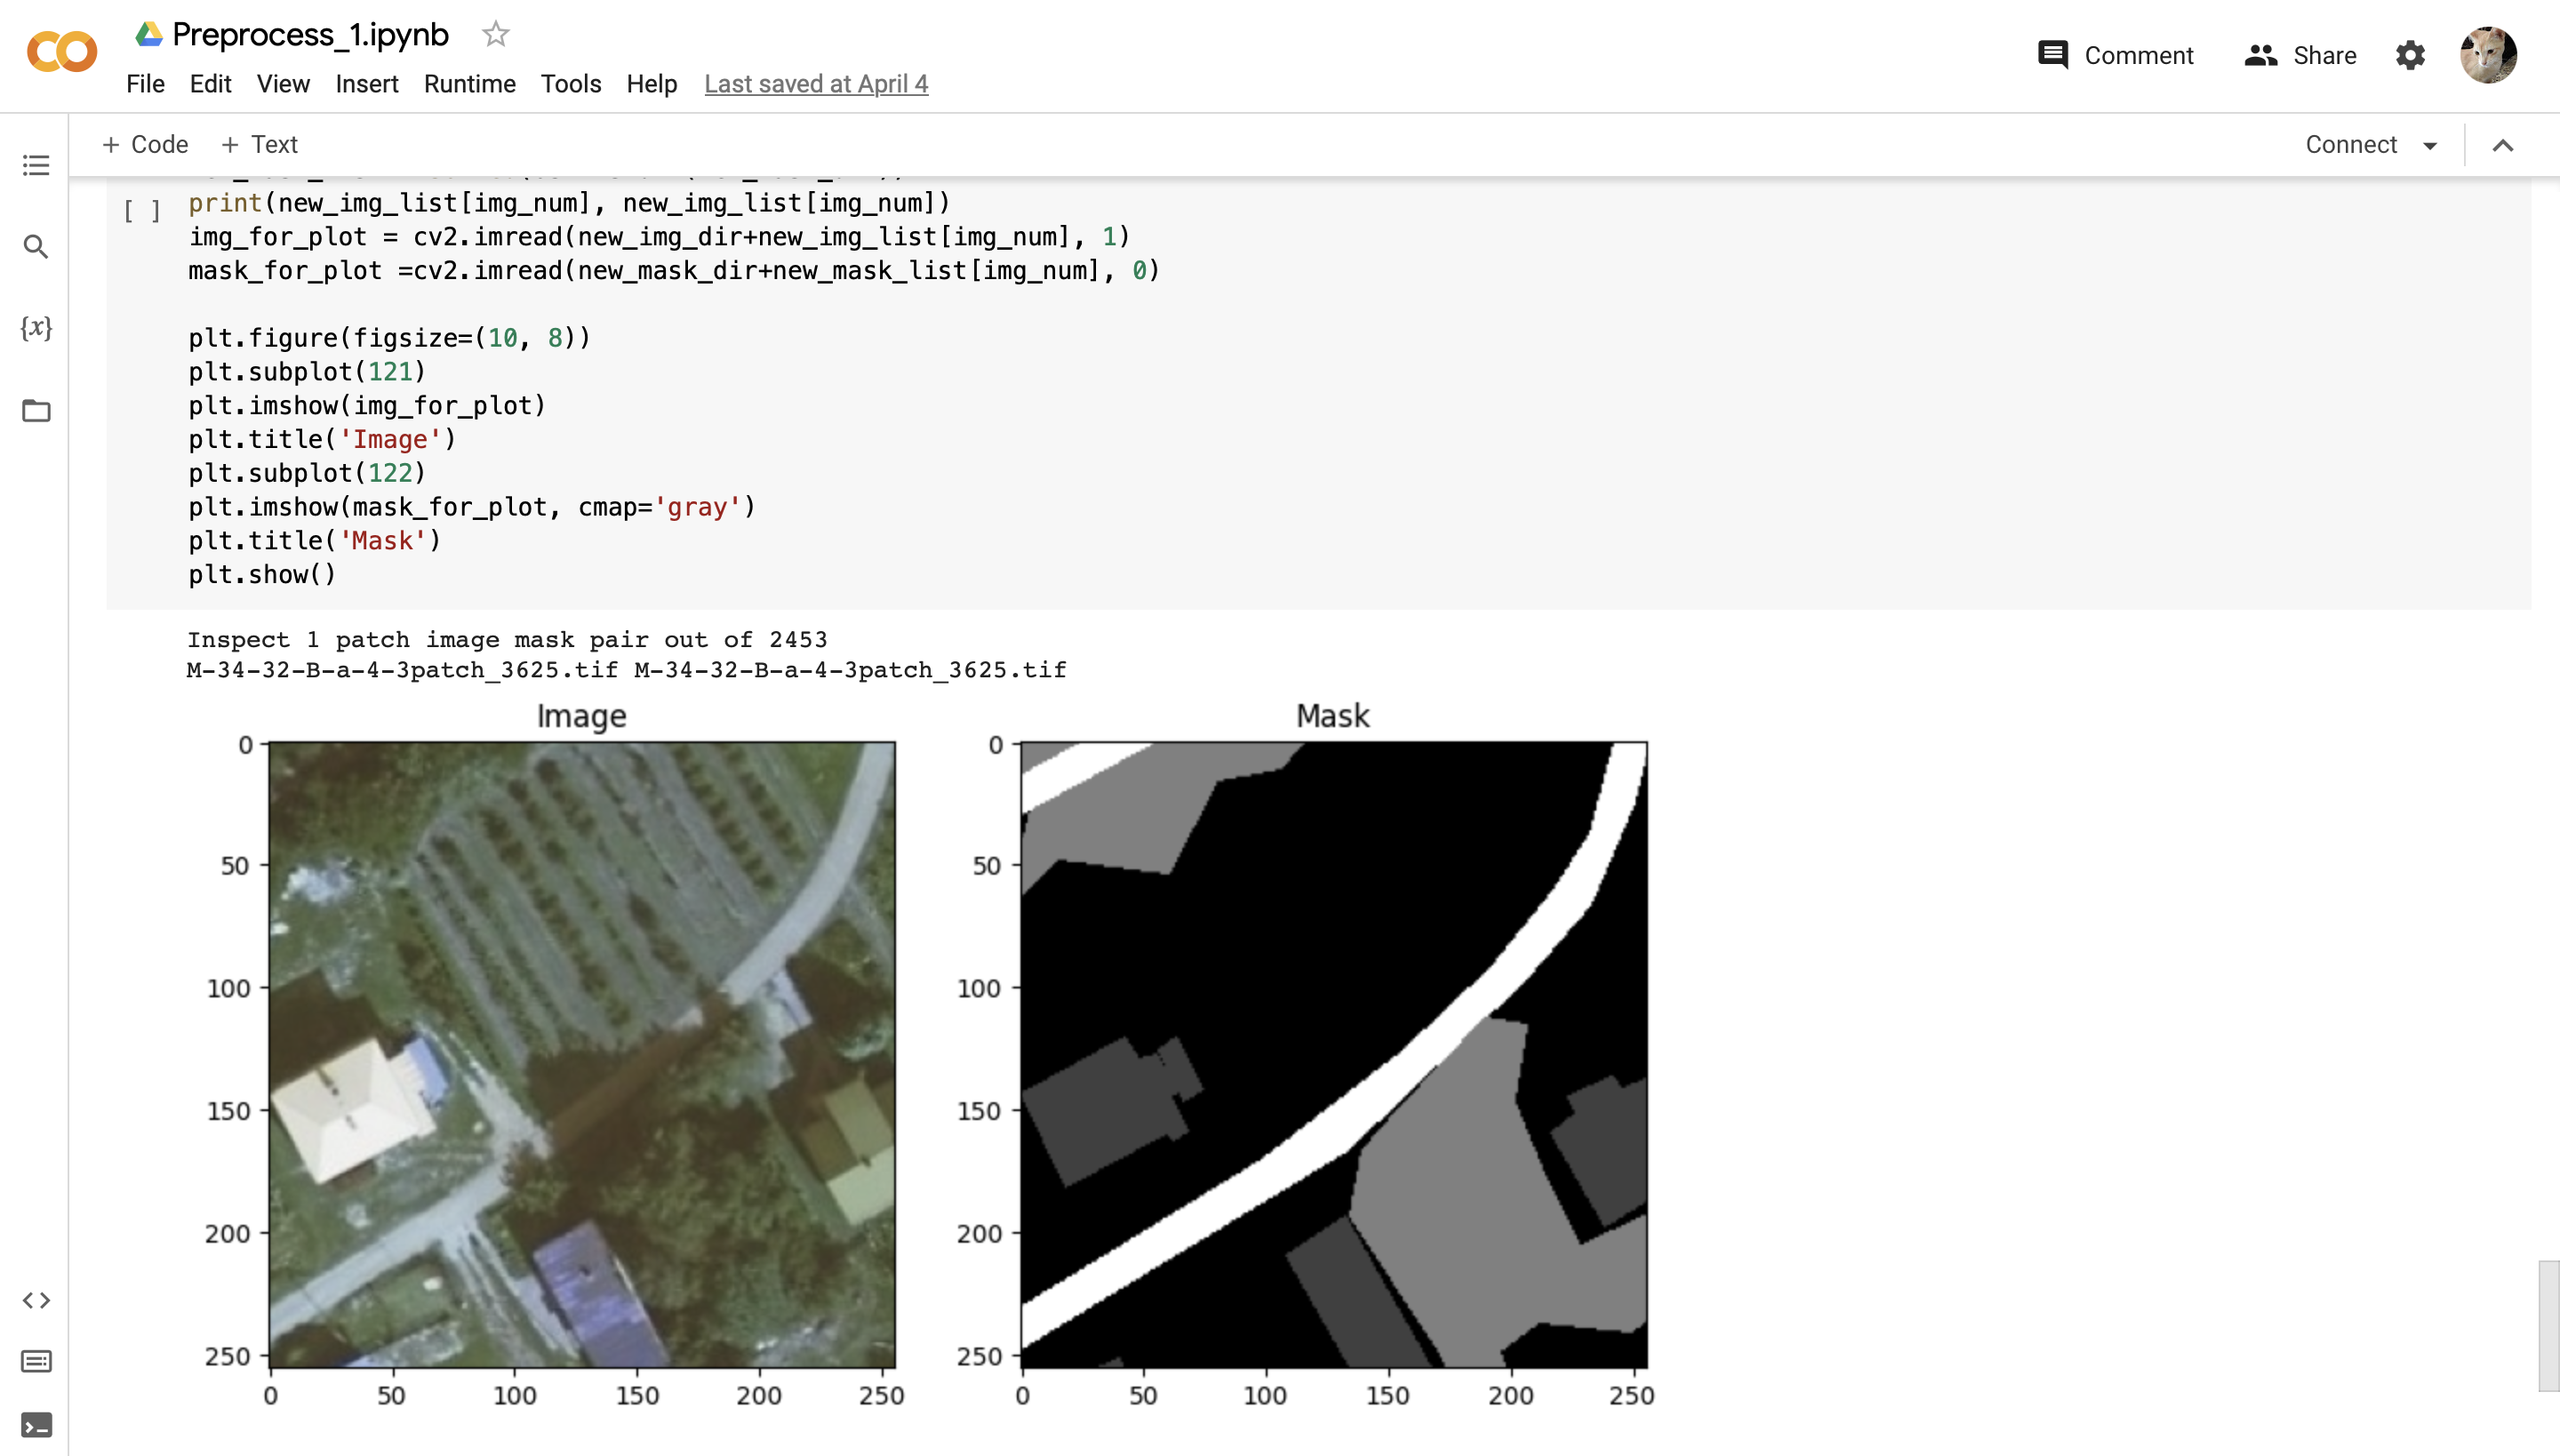
\includegraphics[scale=0.34]{screenshts/9.png}
\section{Training using UNet Architecture}
% 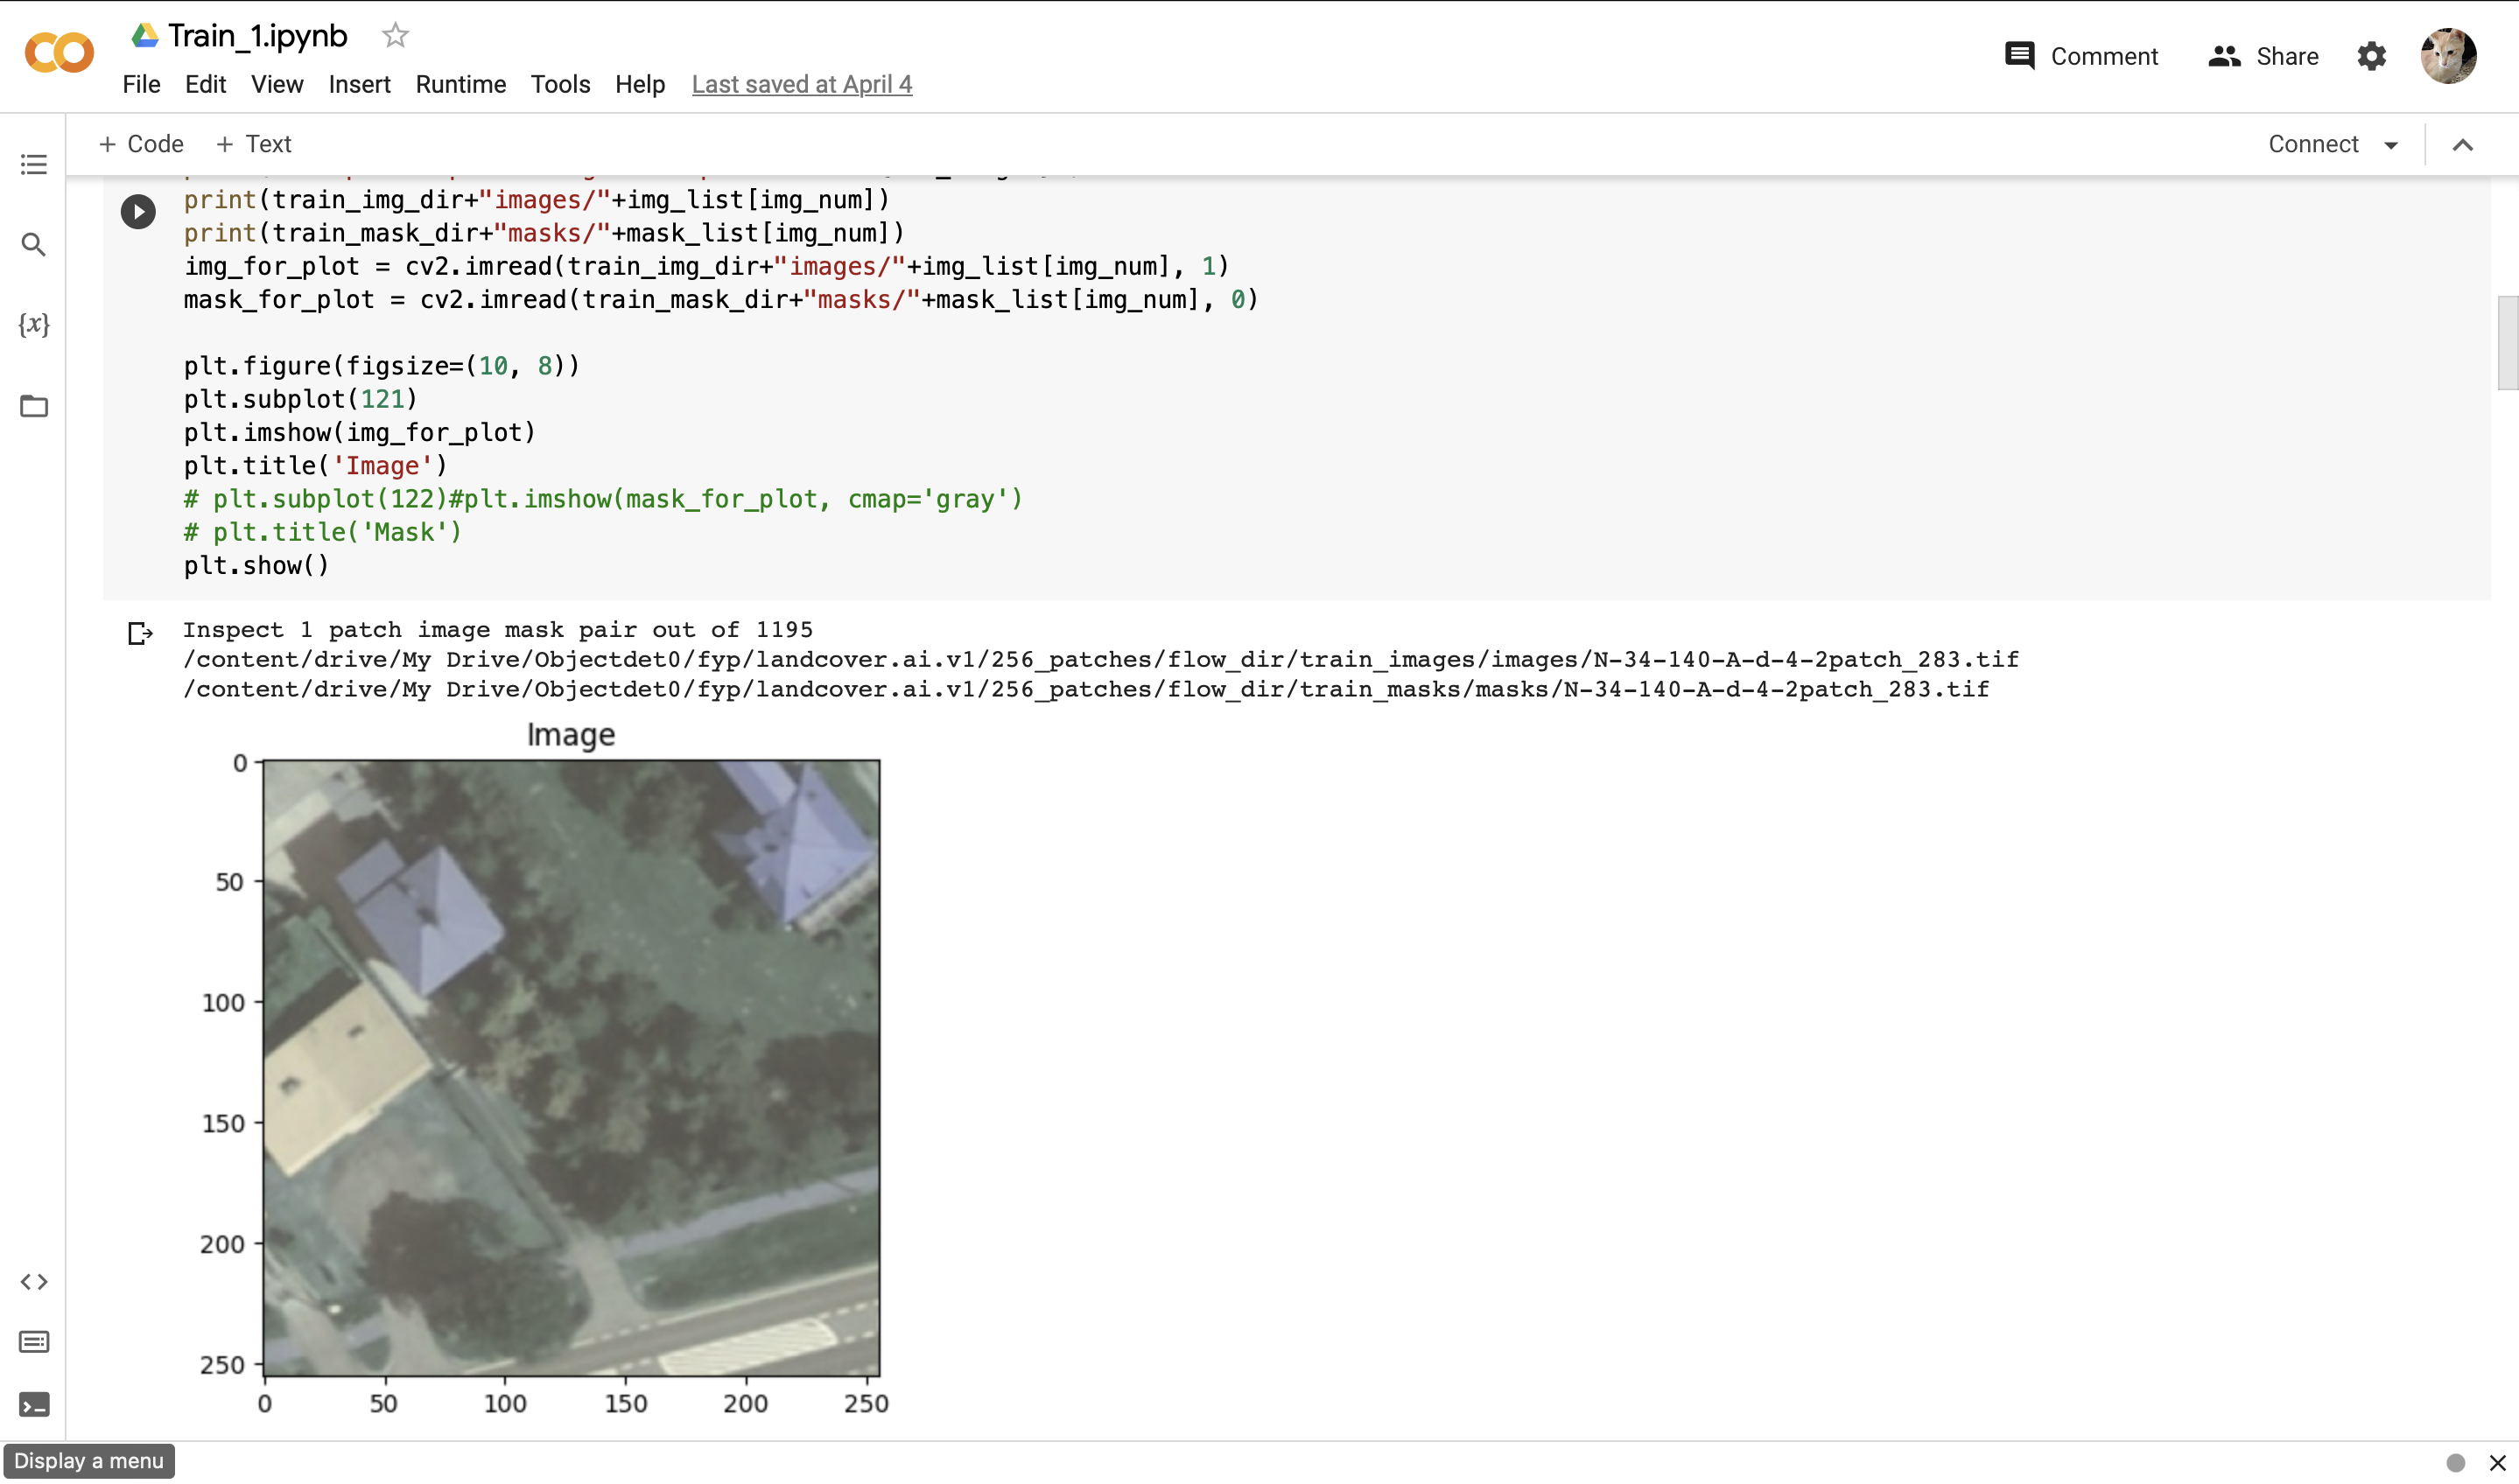
\includegraphics[scale=0.4]{screenshts/10.png}
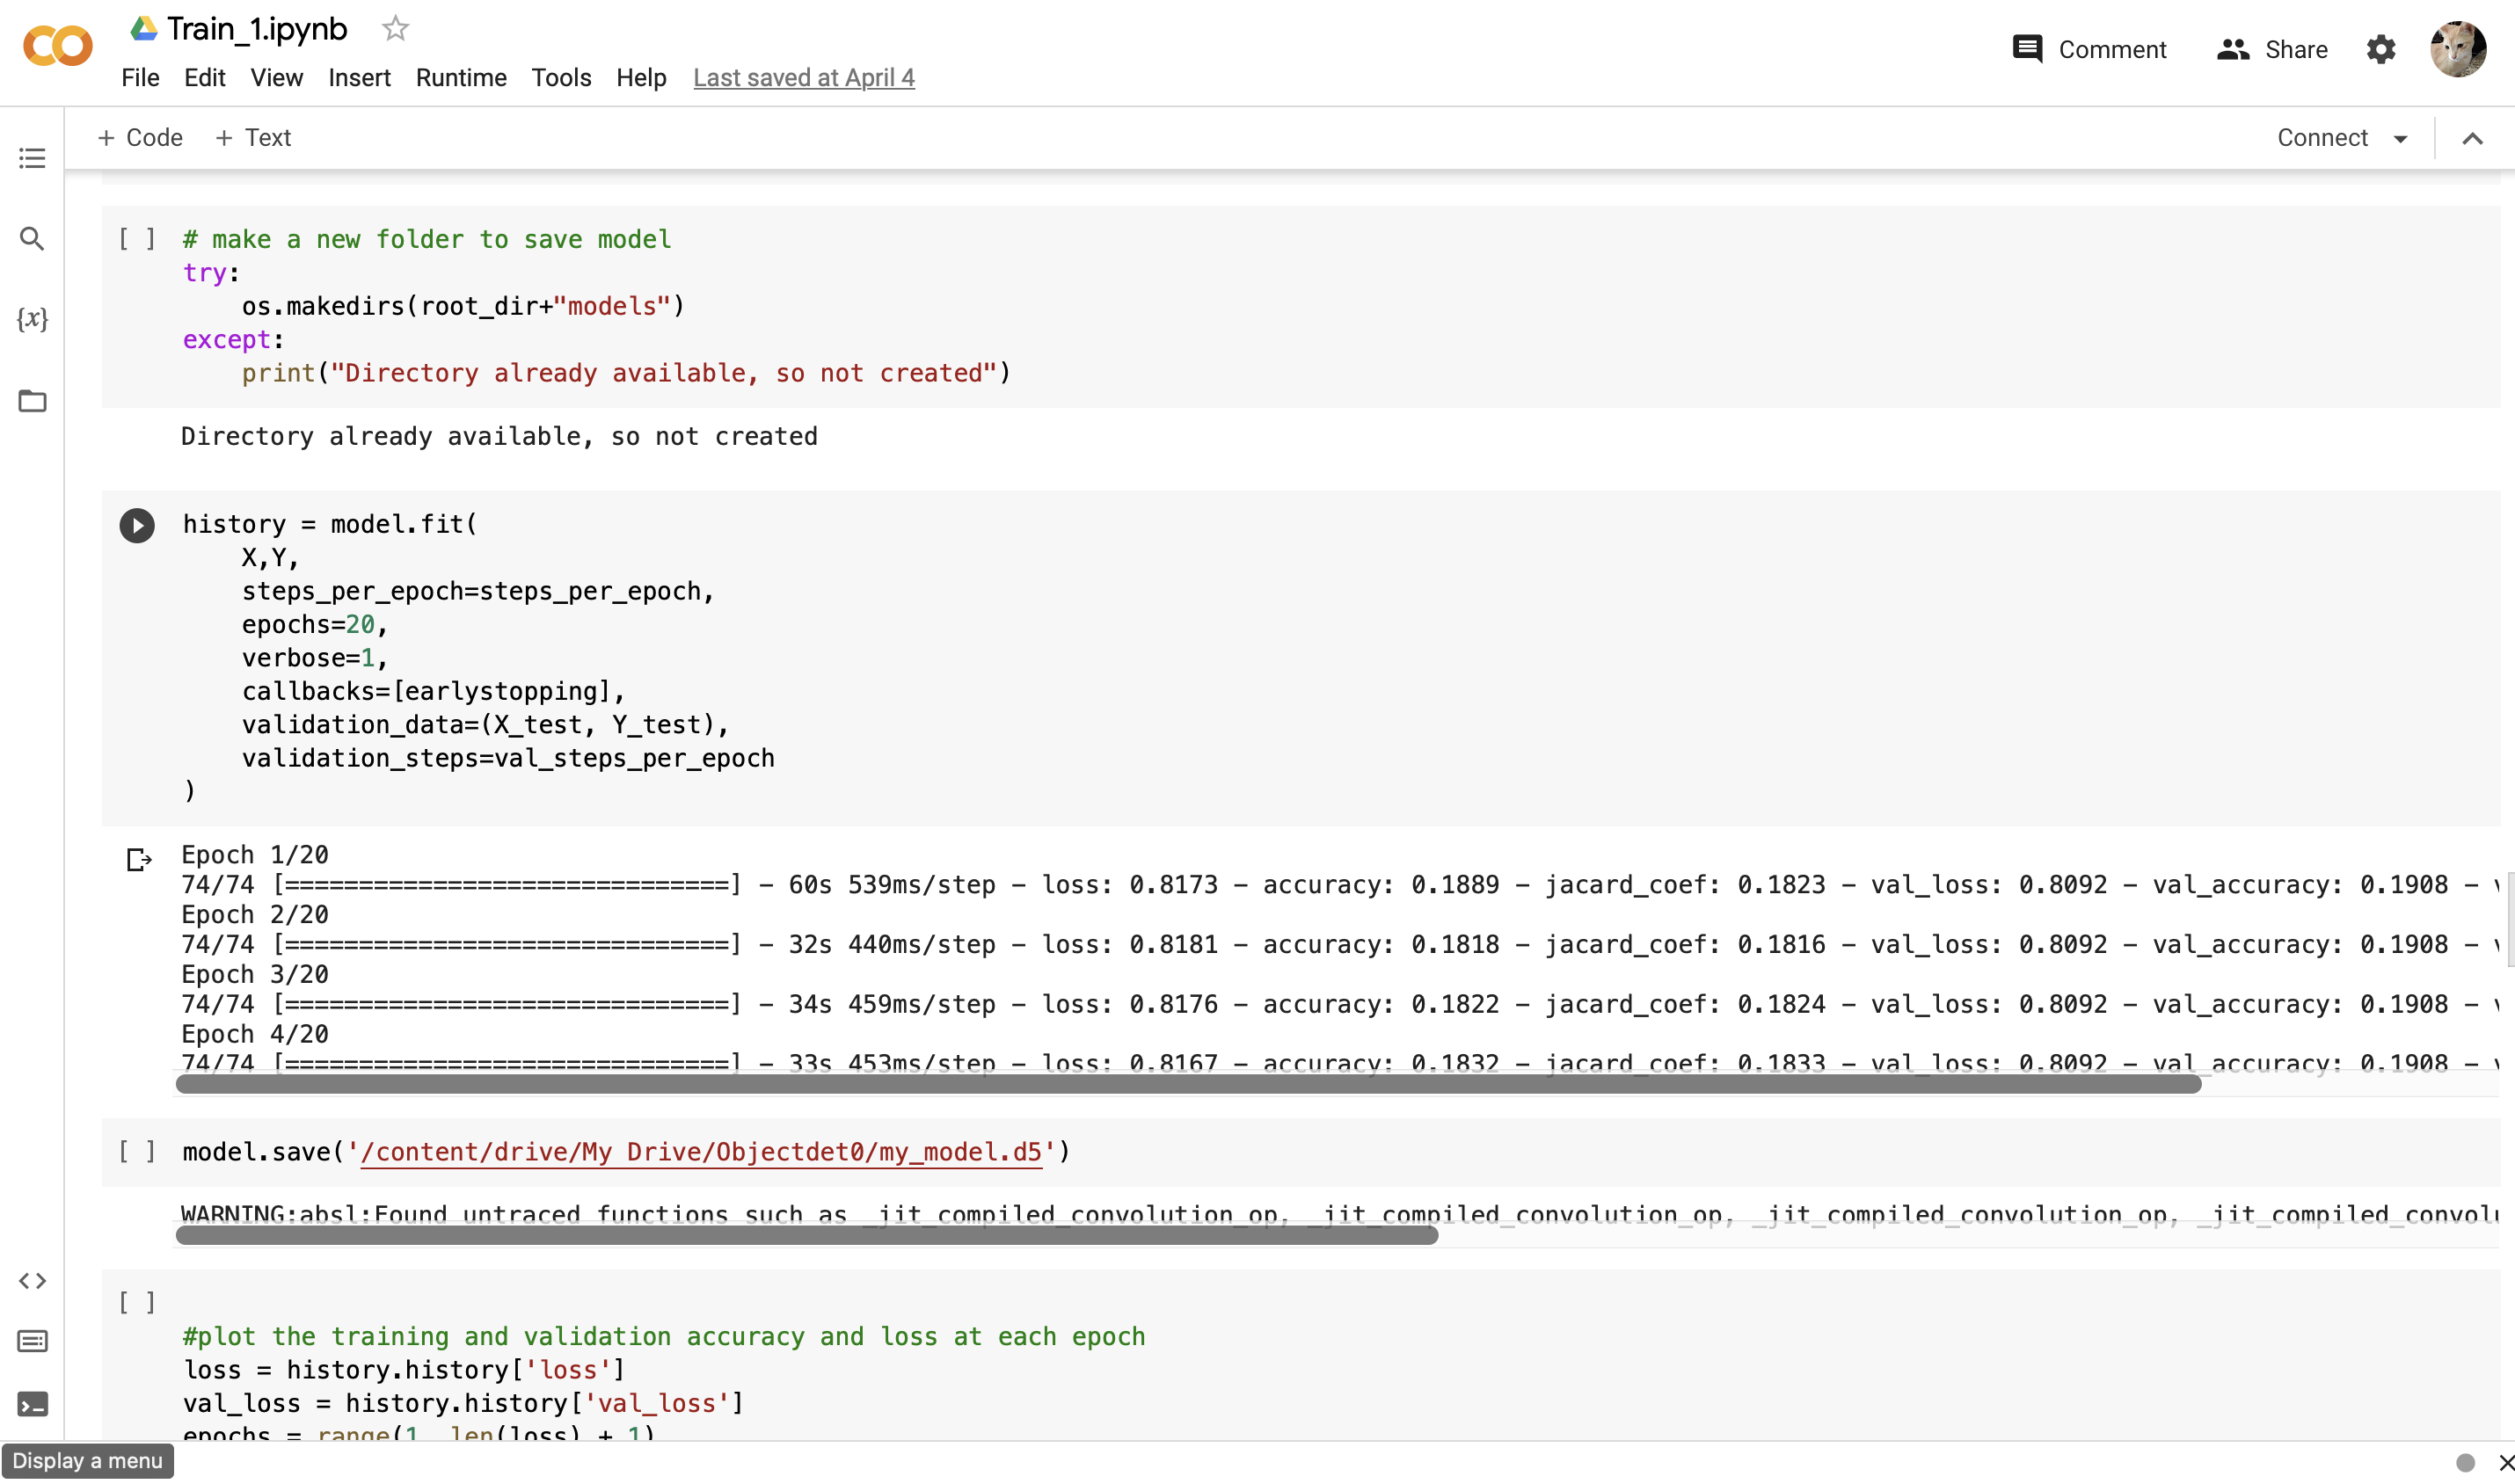
\includegraphics[scale=0.4]{screenshts/11.png}
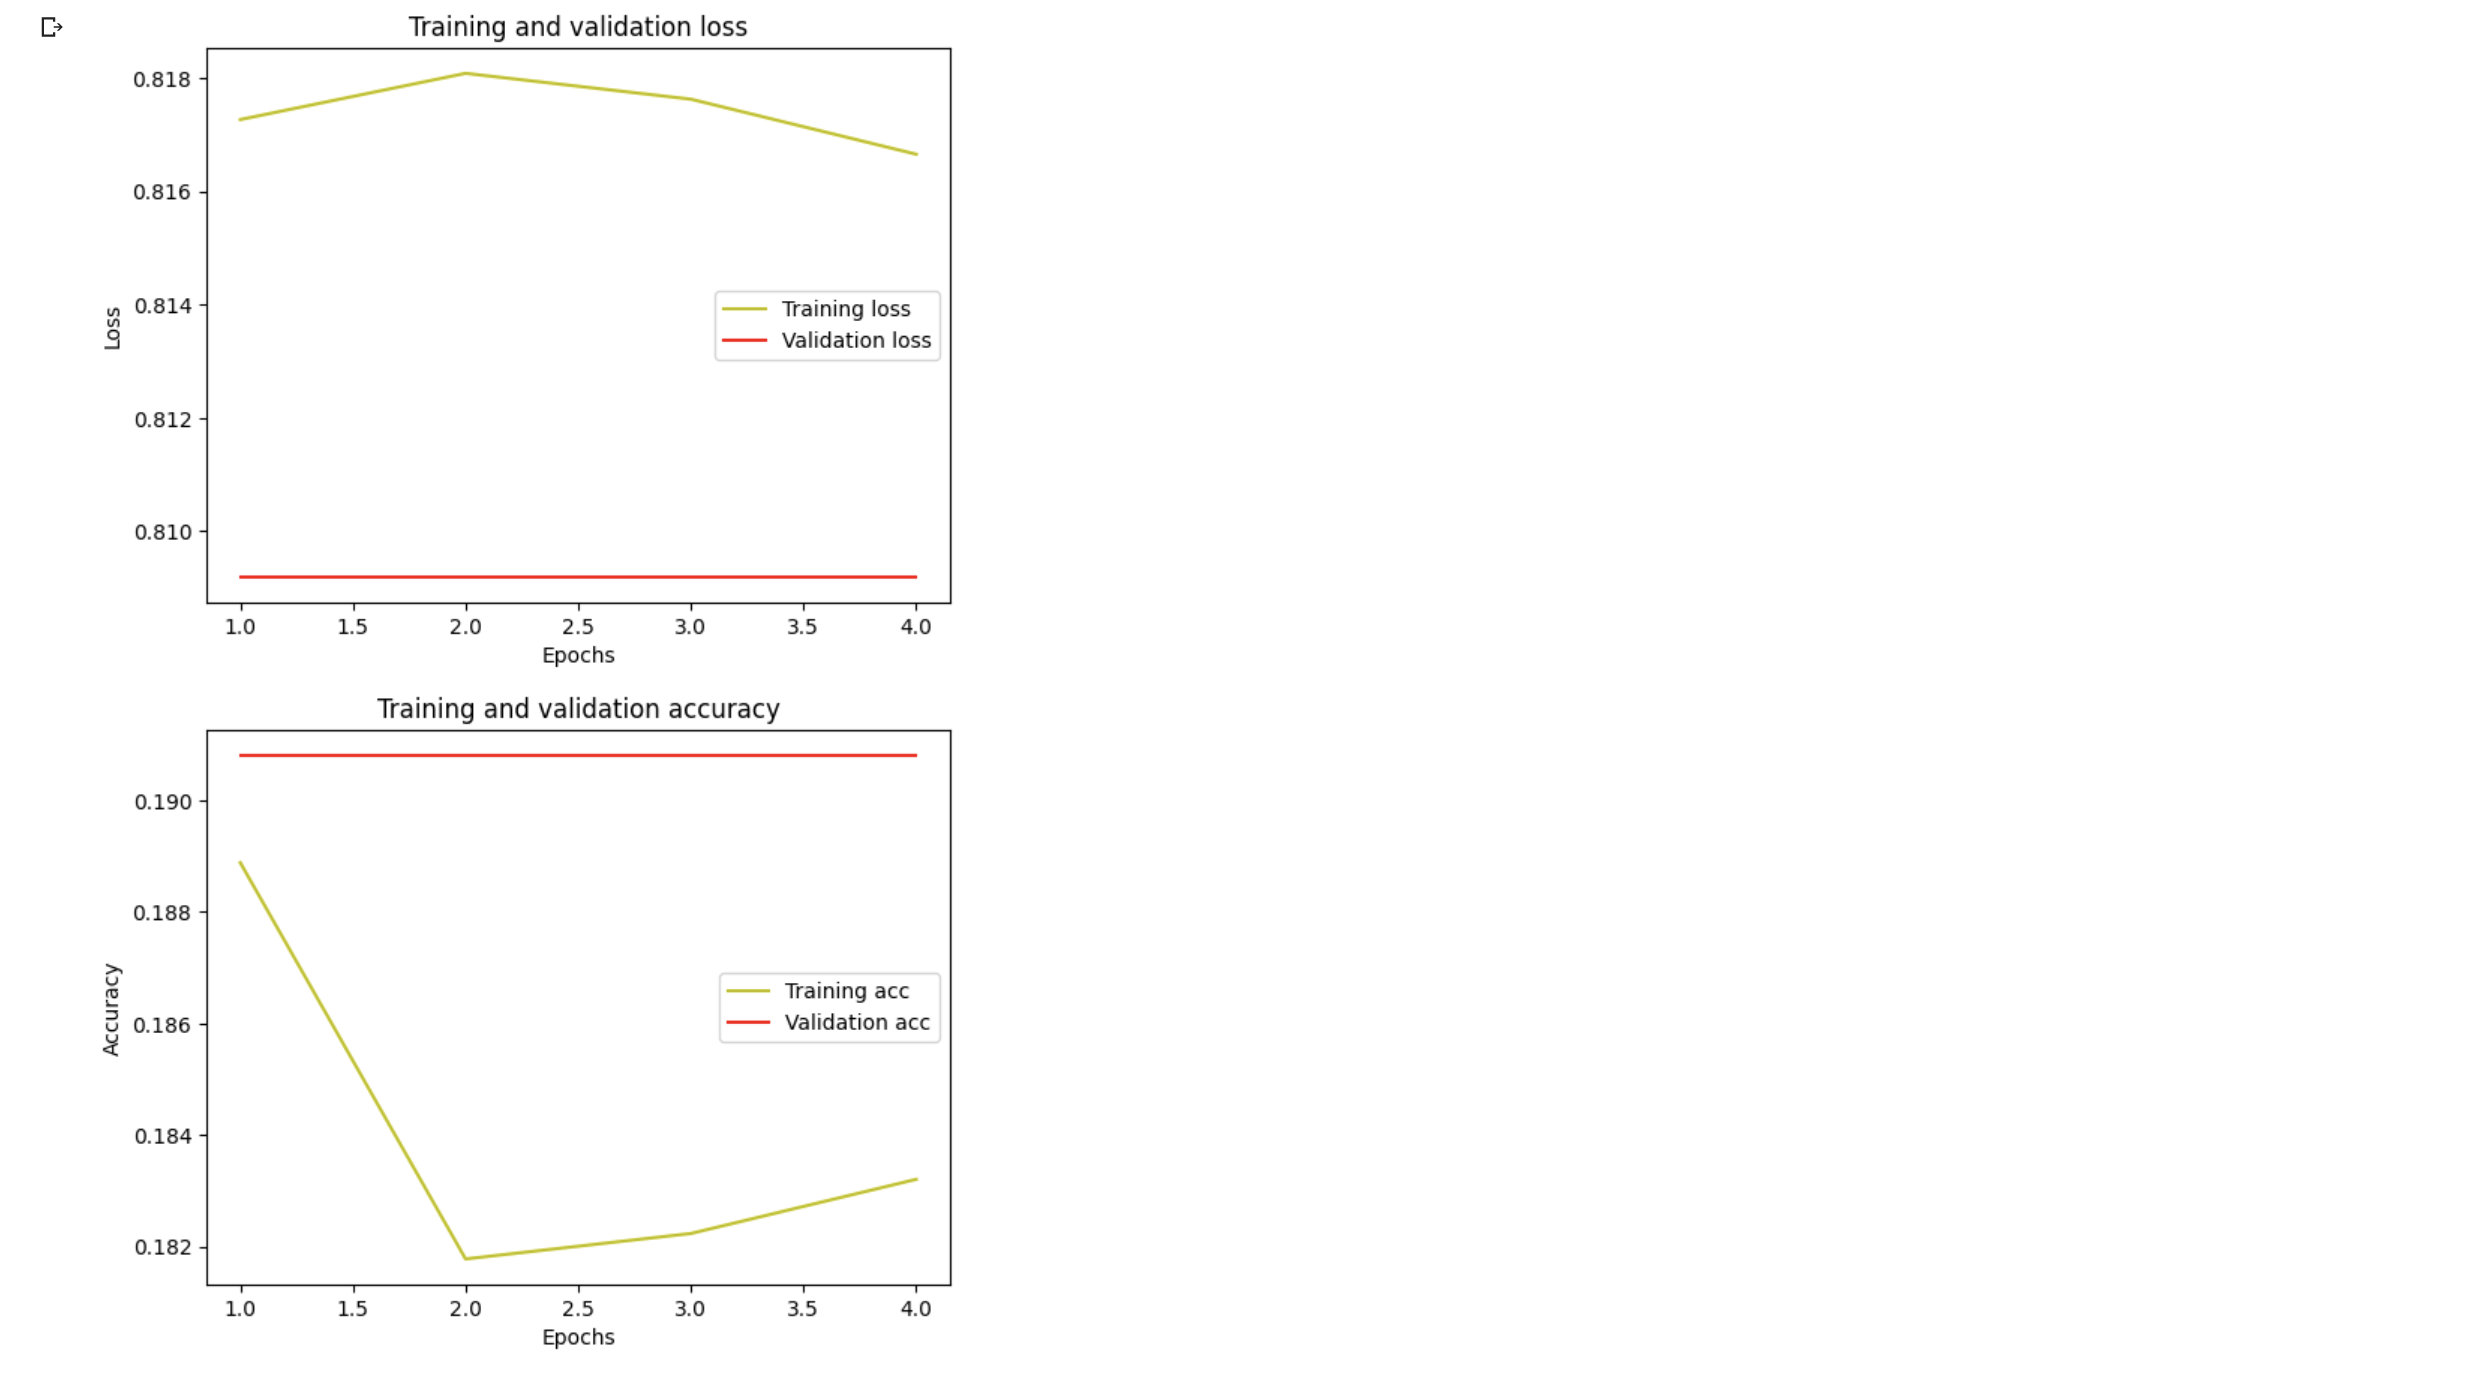
\includegraphics[scale=0.4]{screenshts/12.png}
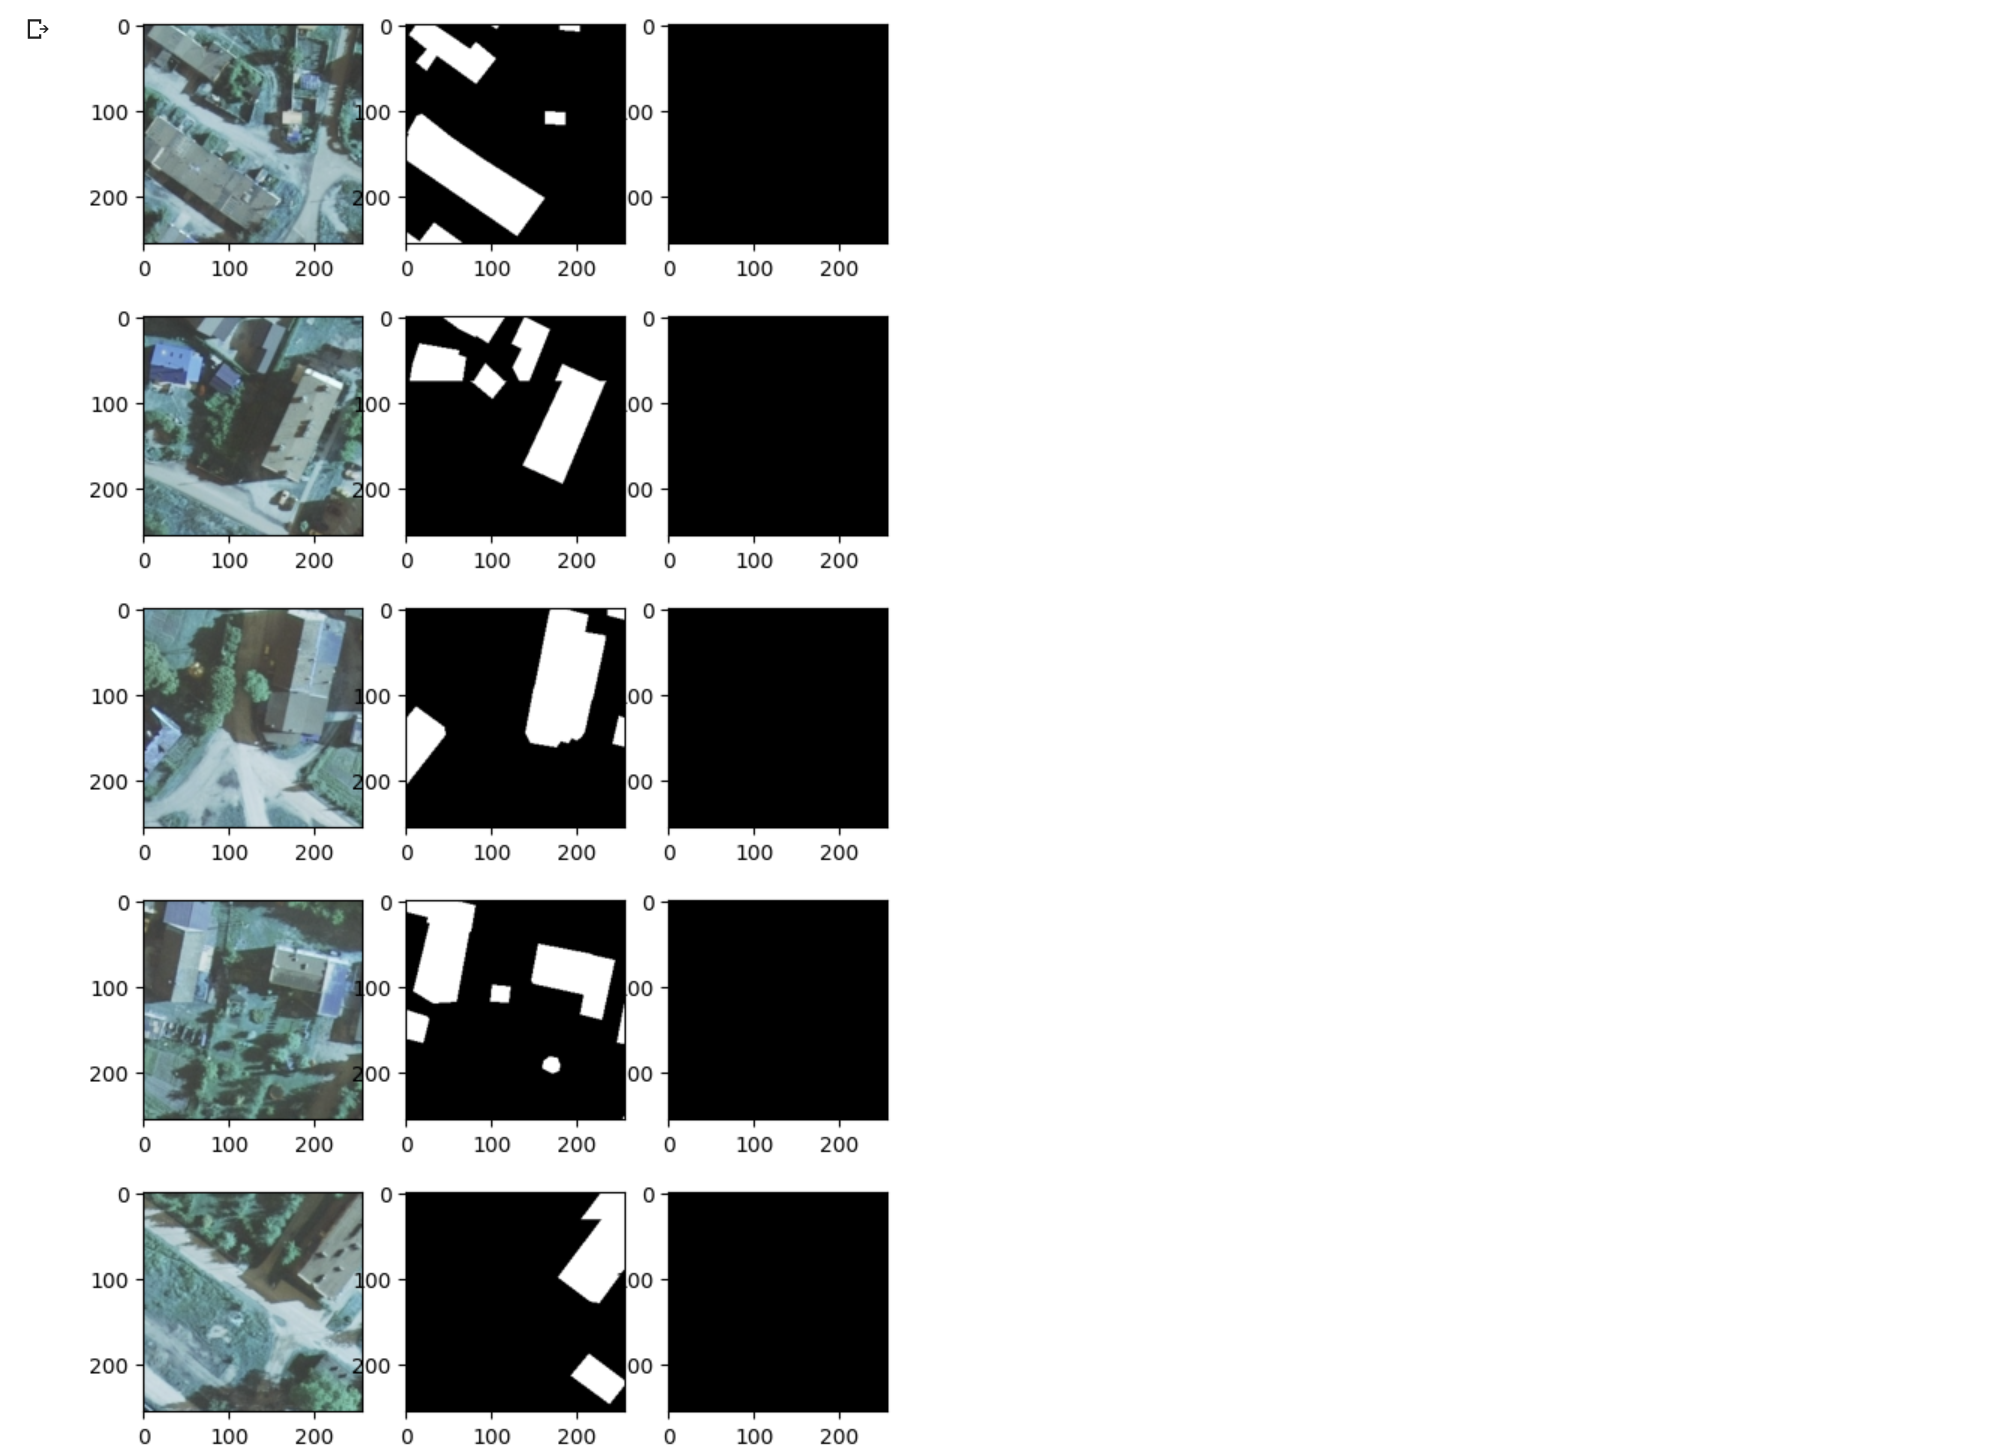
\includegraphics[scale=0.6]{screenshts/13.png}

\section{Connection to GCP Cloud using key.json}
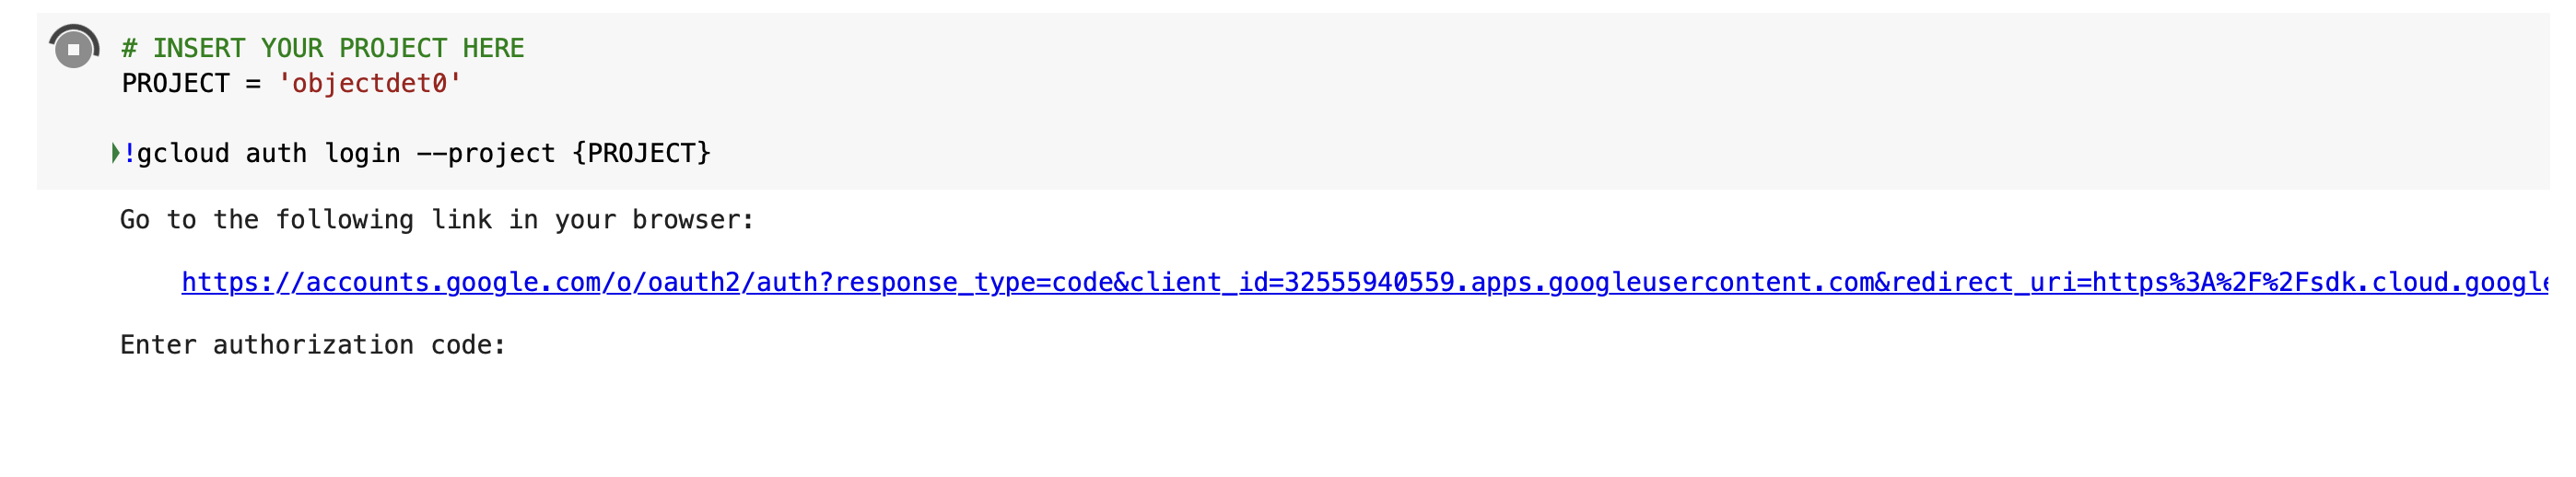
\includegraphics[scale=0.4]{screenshts/14.png}
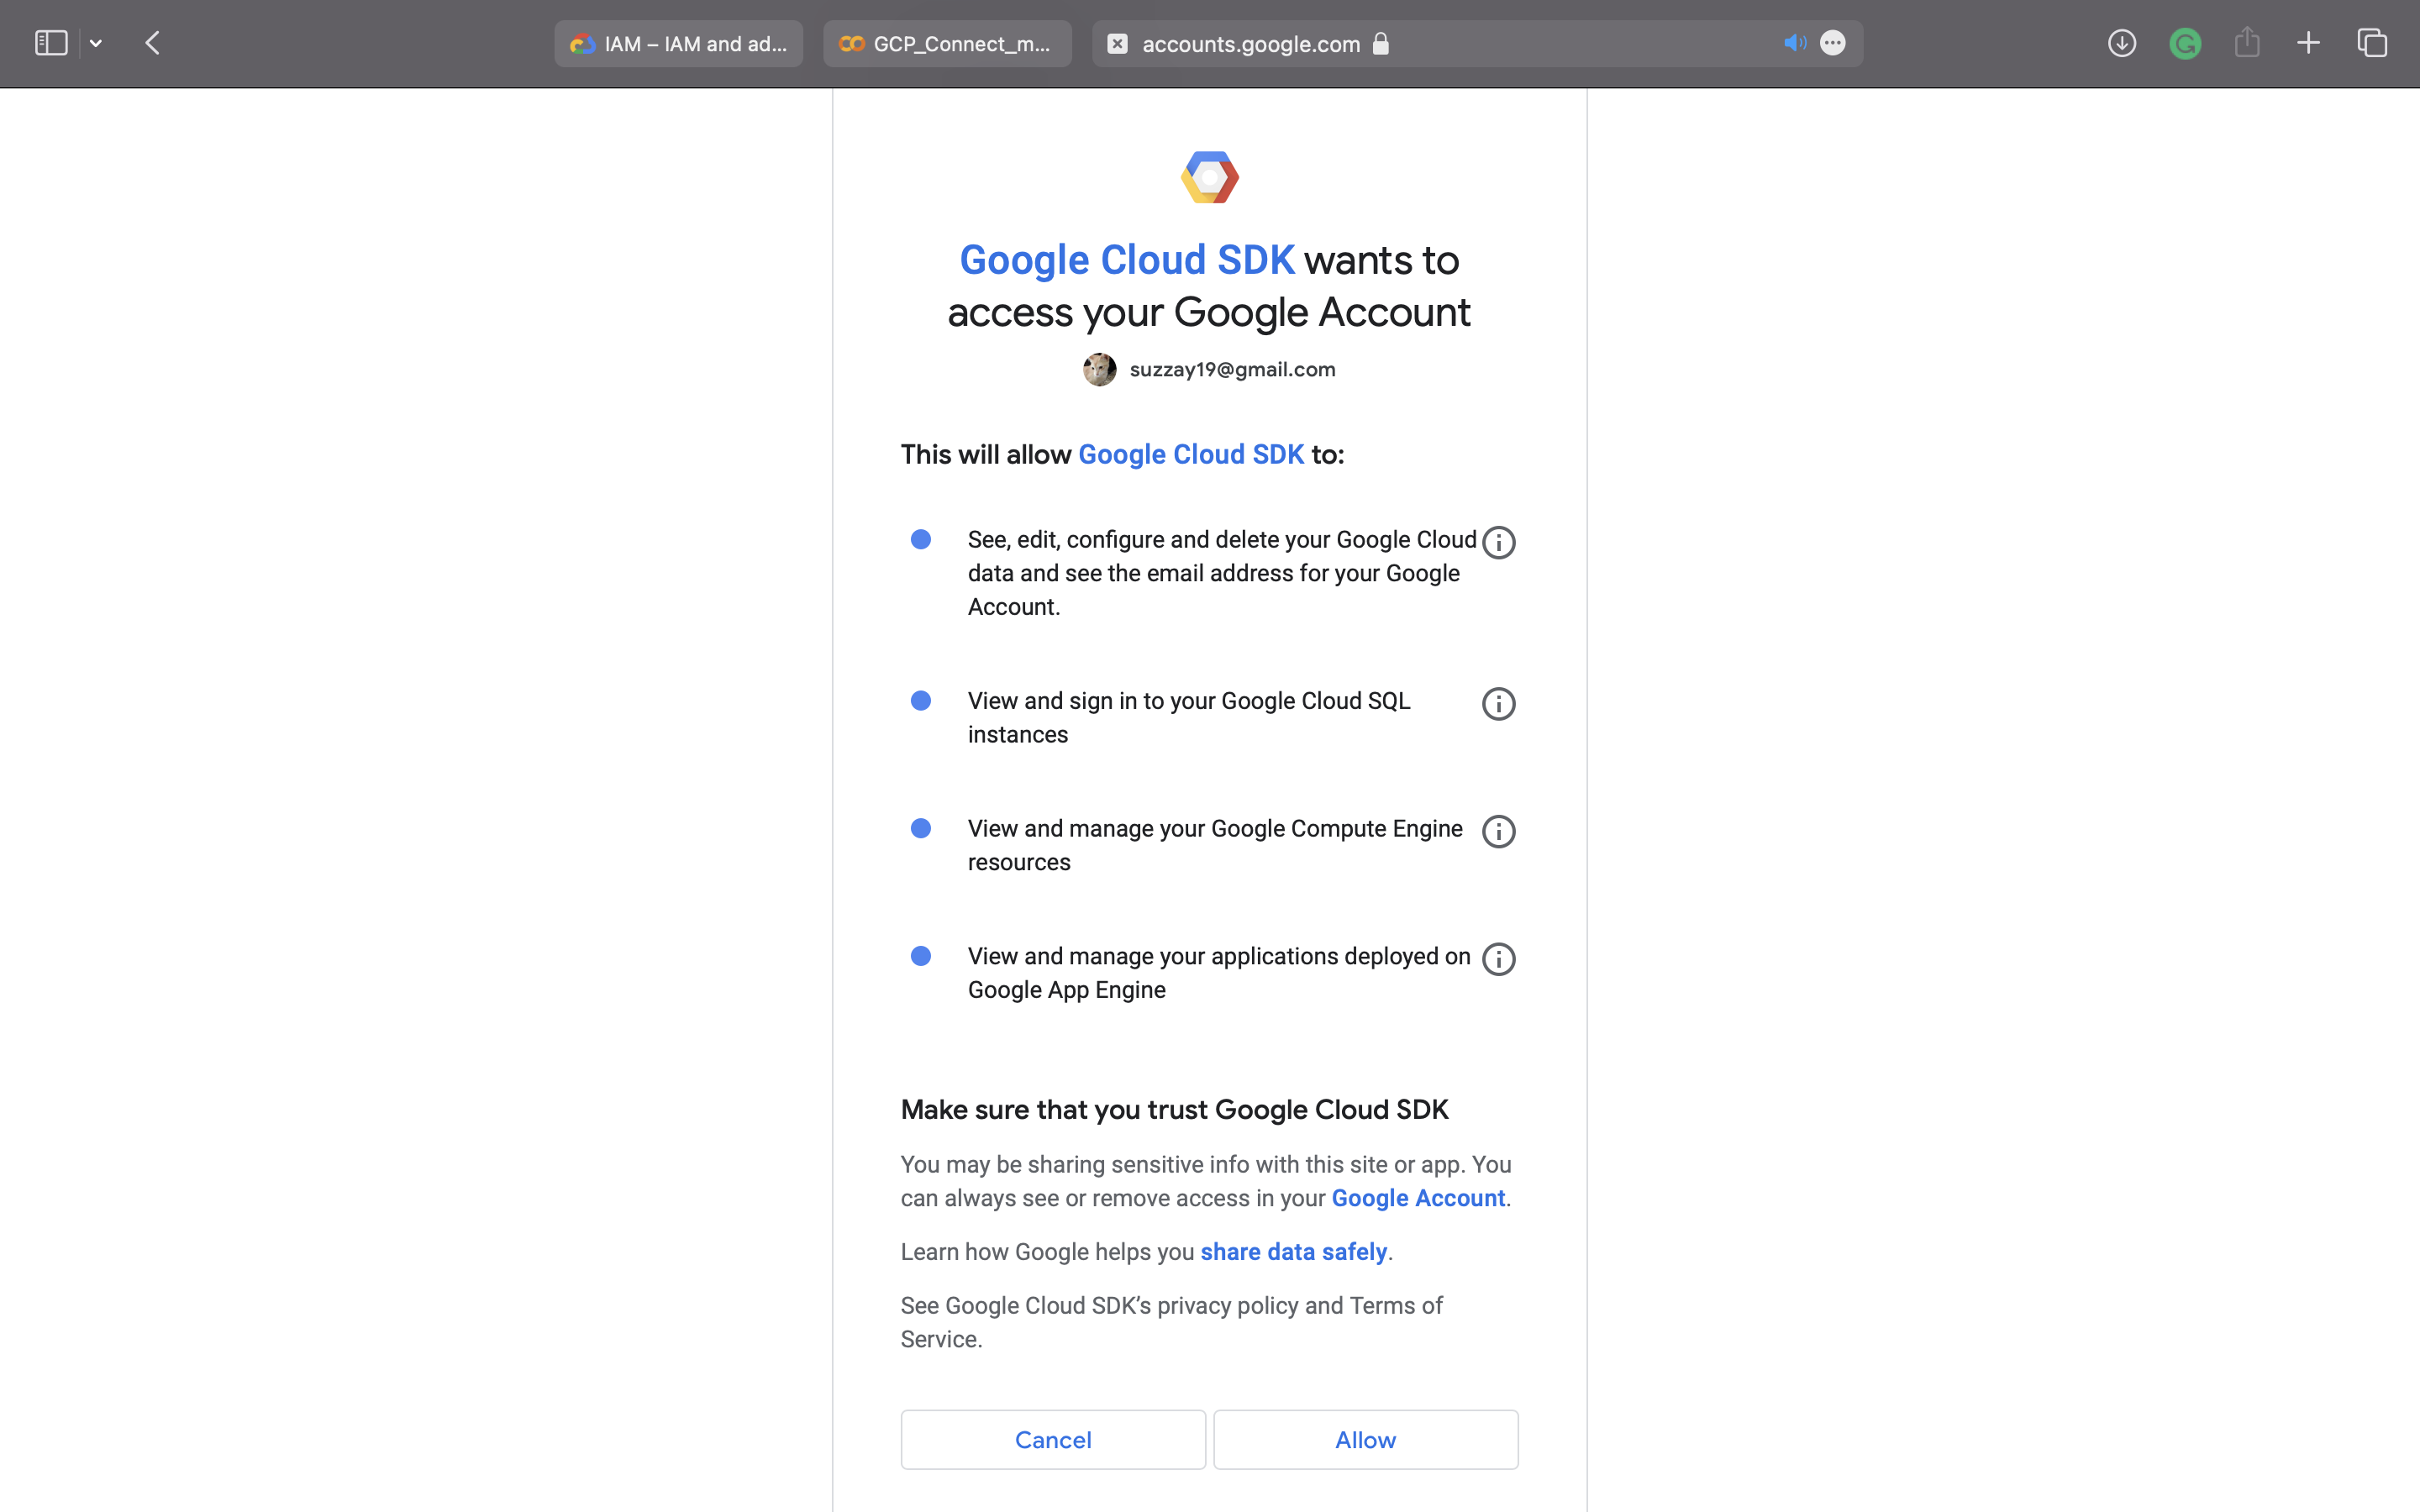
\includegraphics[scale=0.4]{screenshts/15.png}
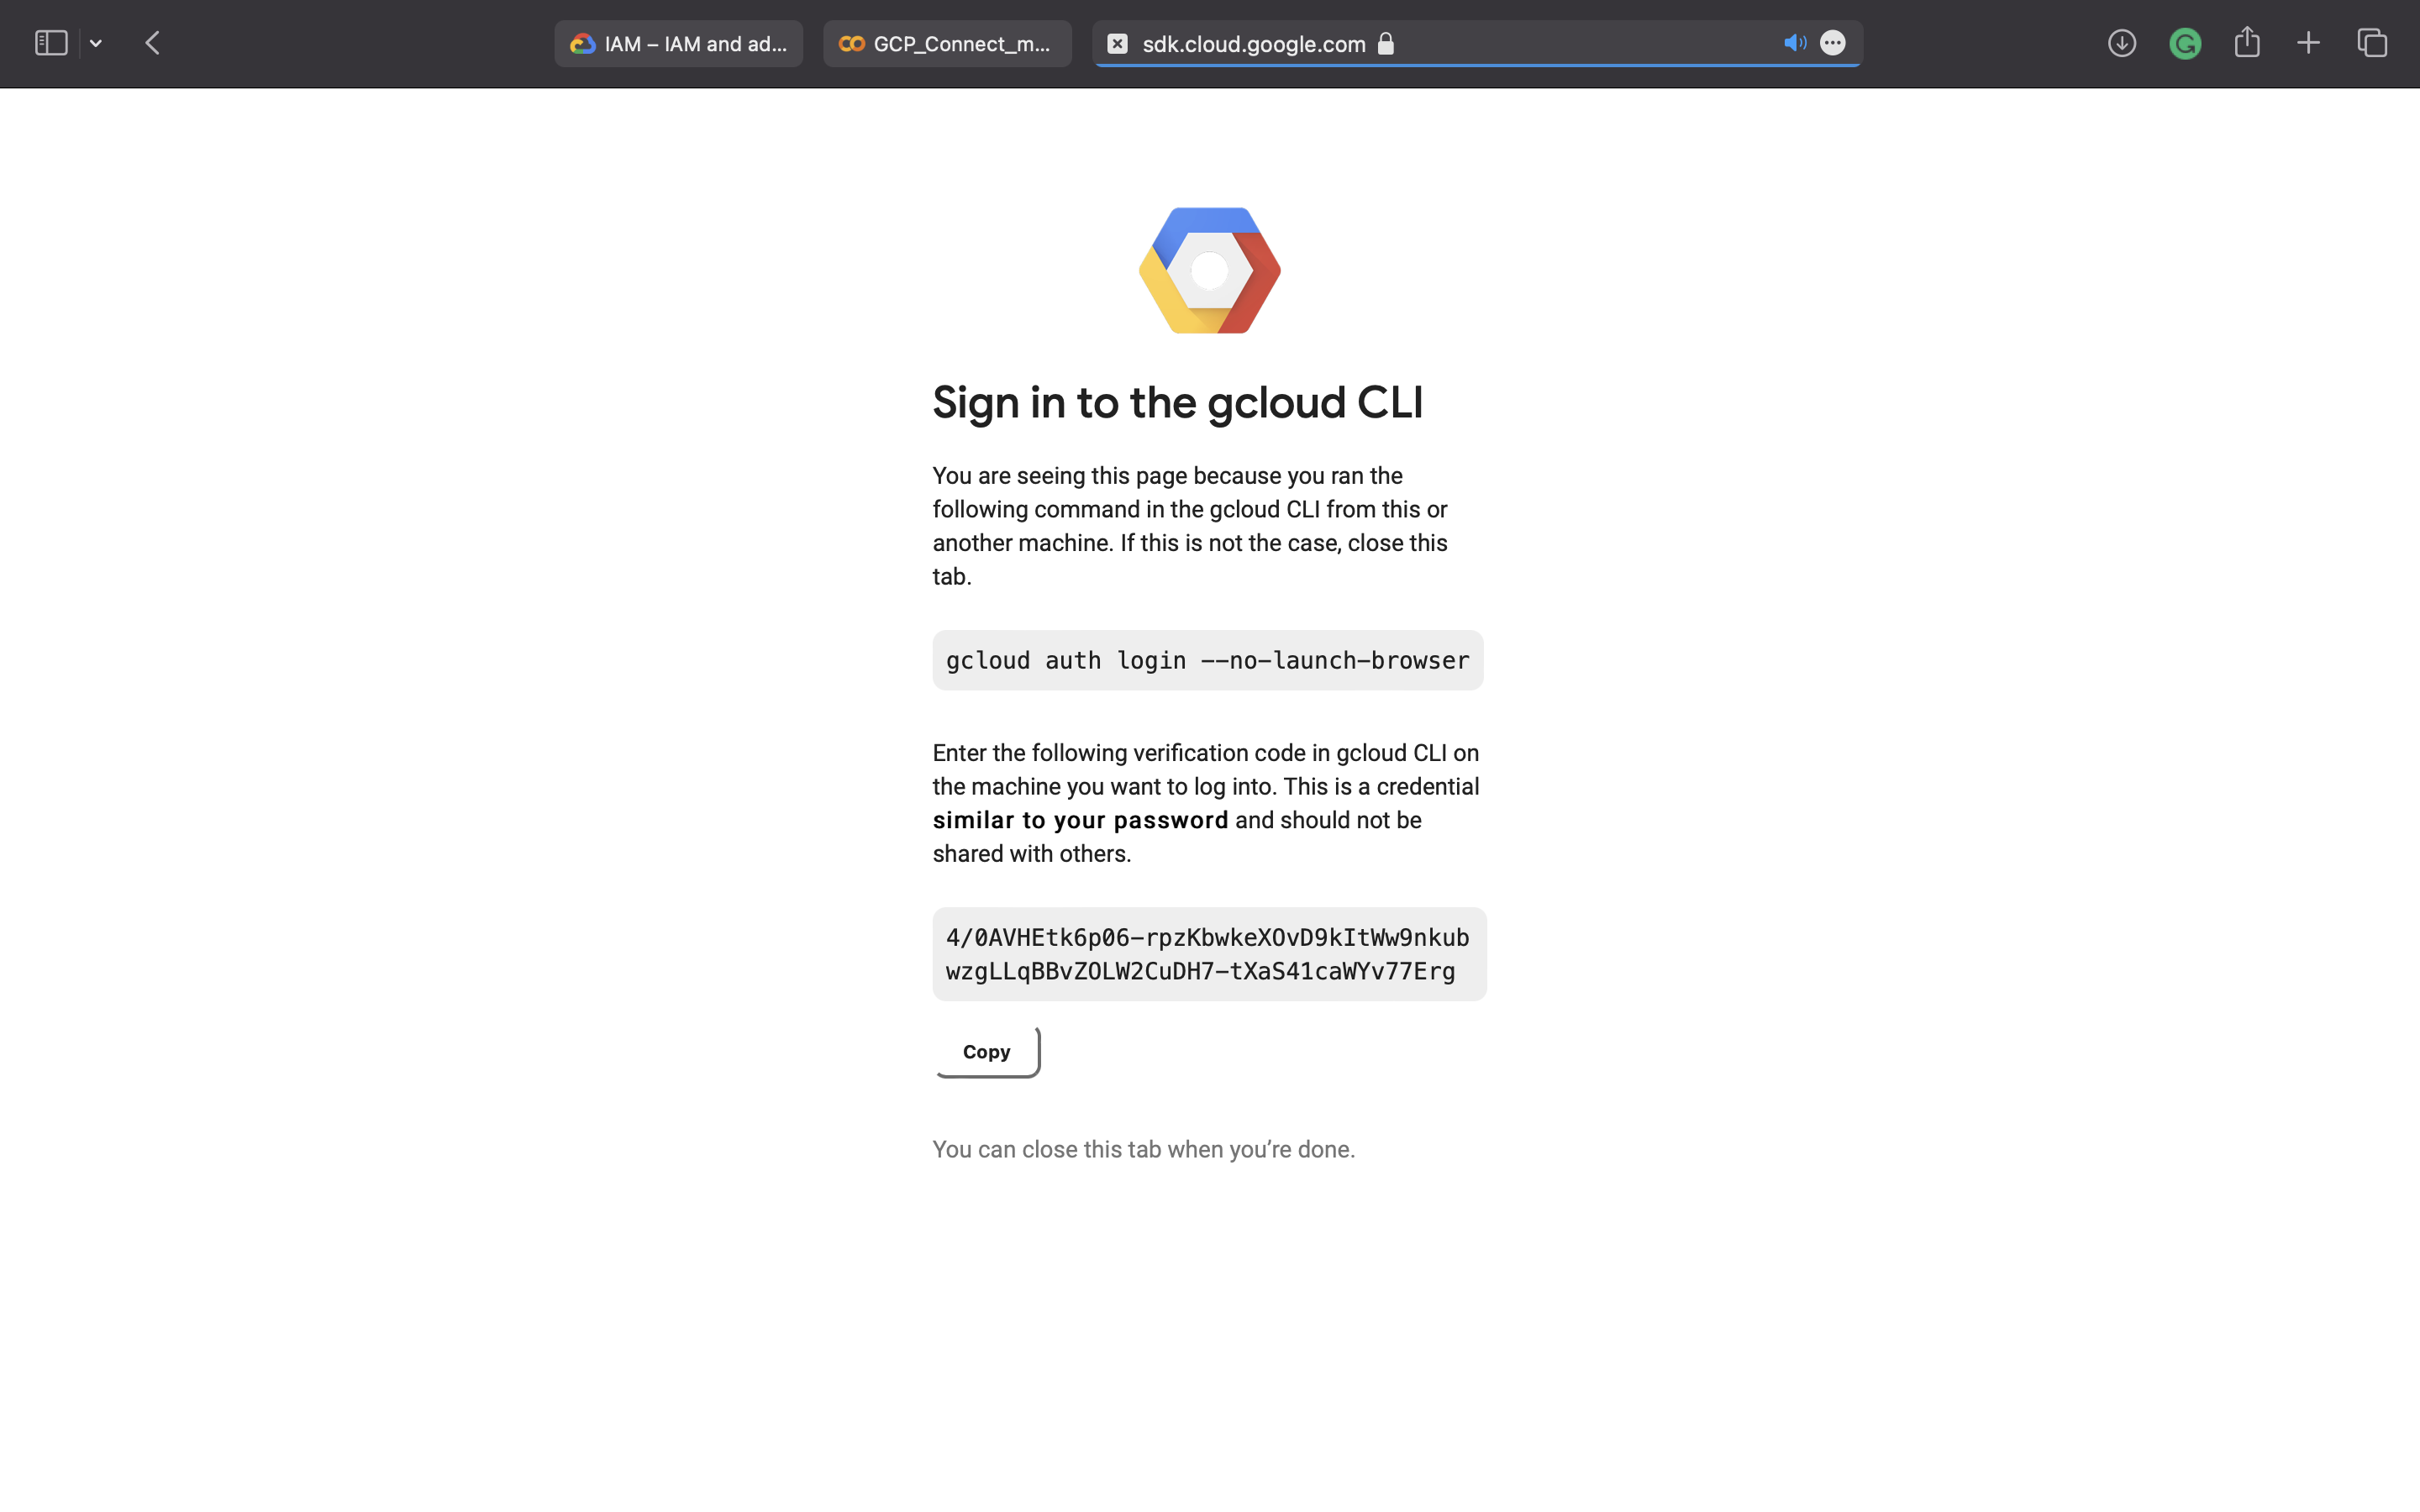
\includegraphics[scale=0.4]{screenshts/16.png}
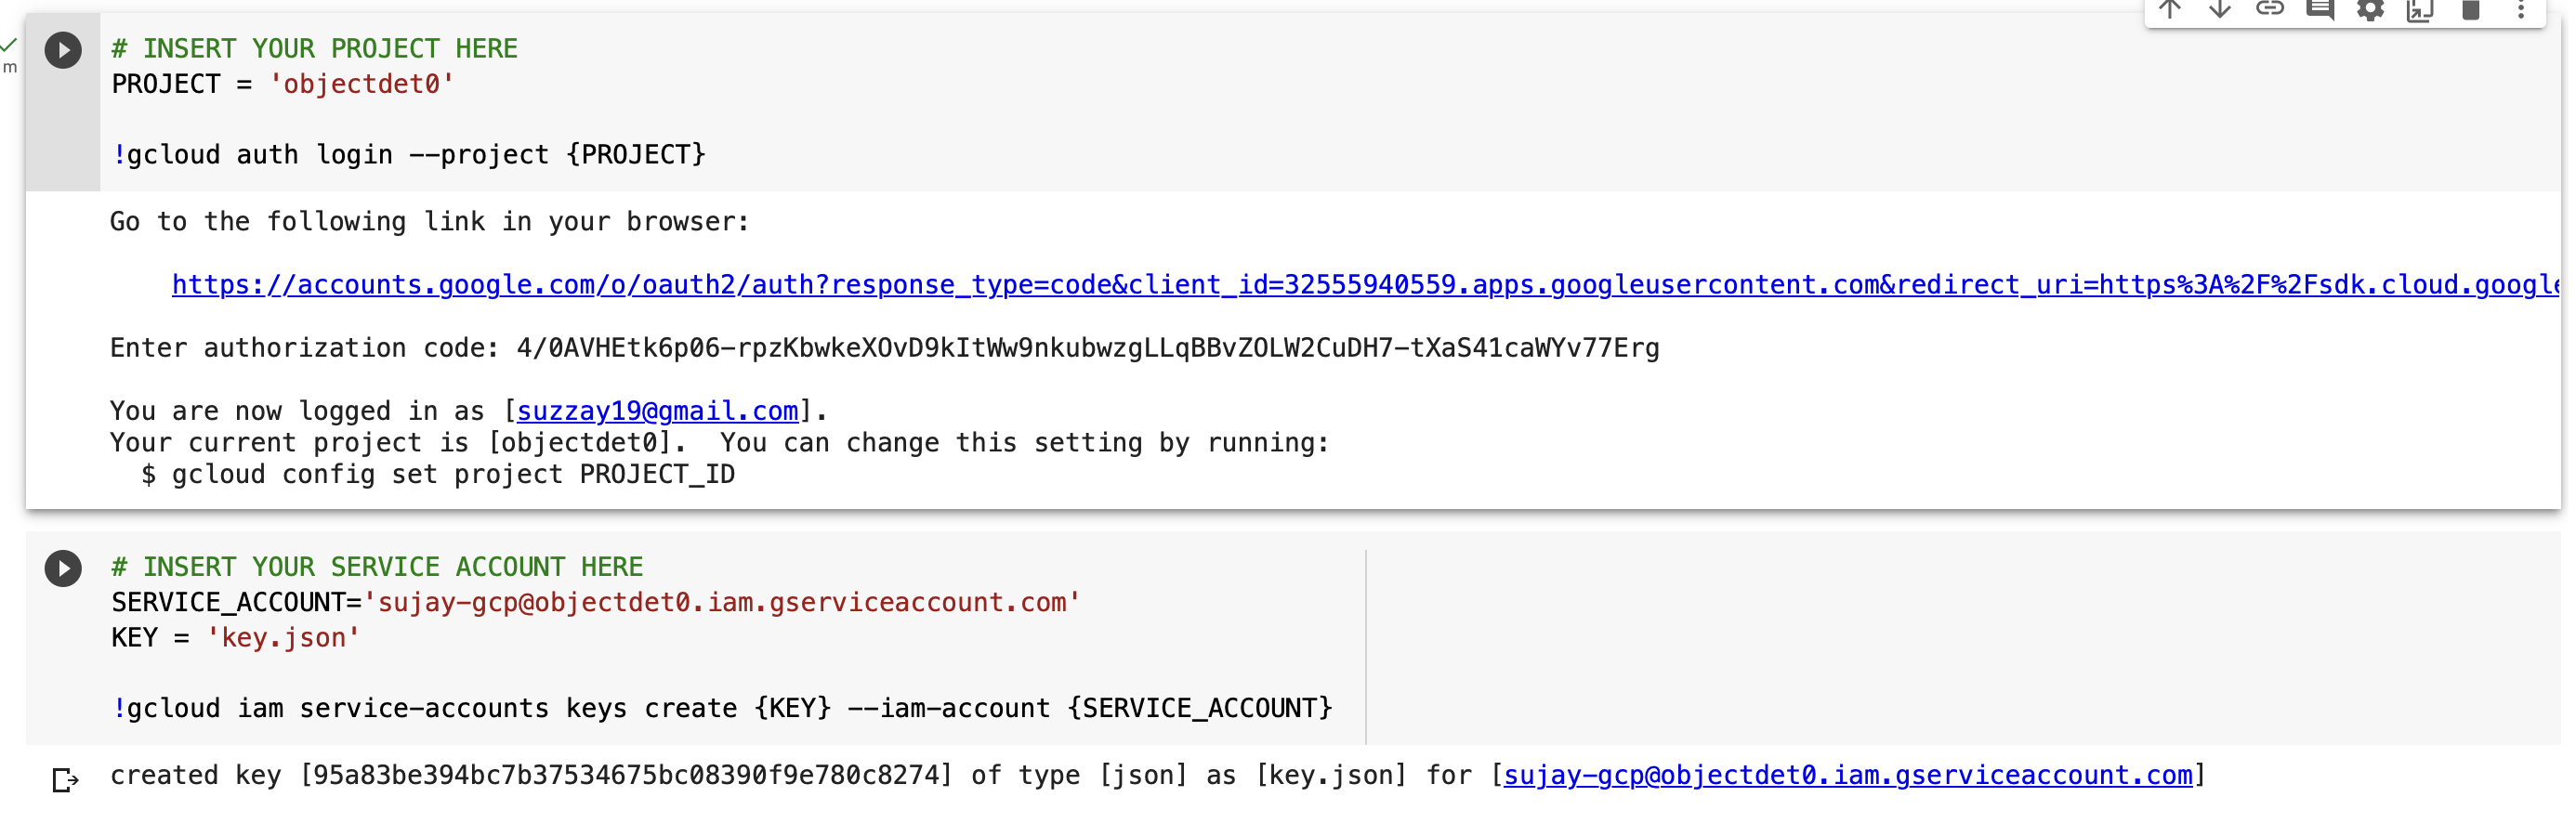
\includegraphics[scale=0.4]{screenshts/17.png}
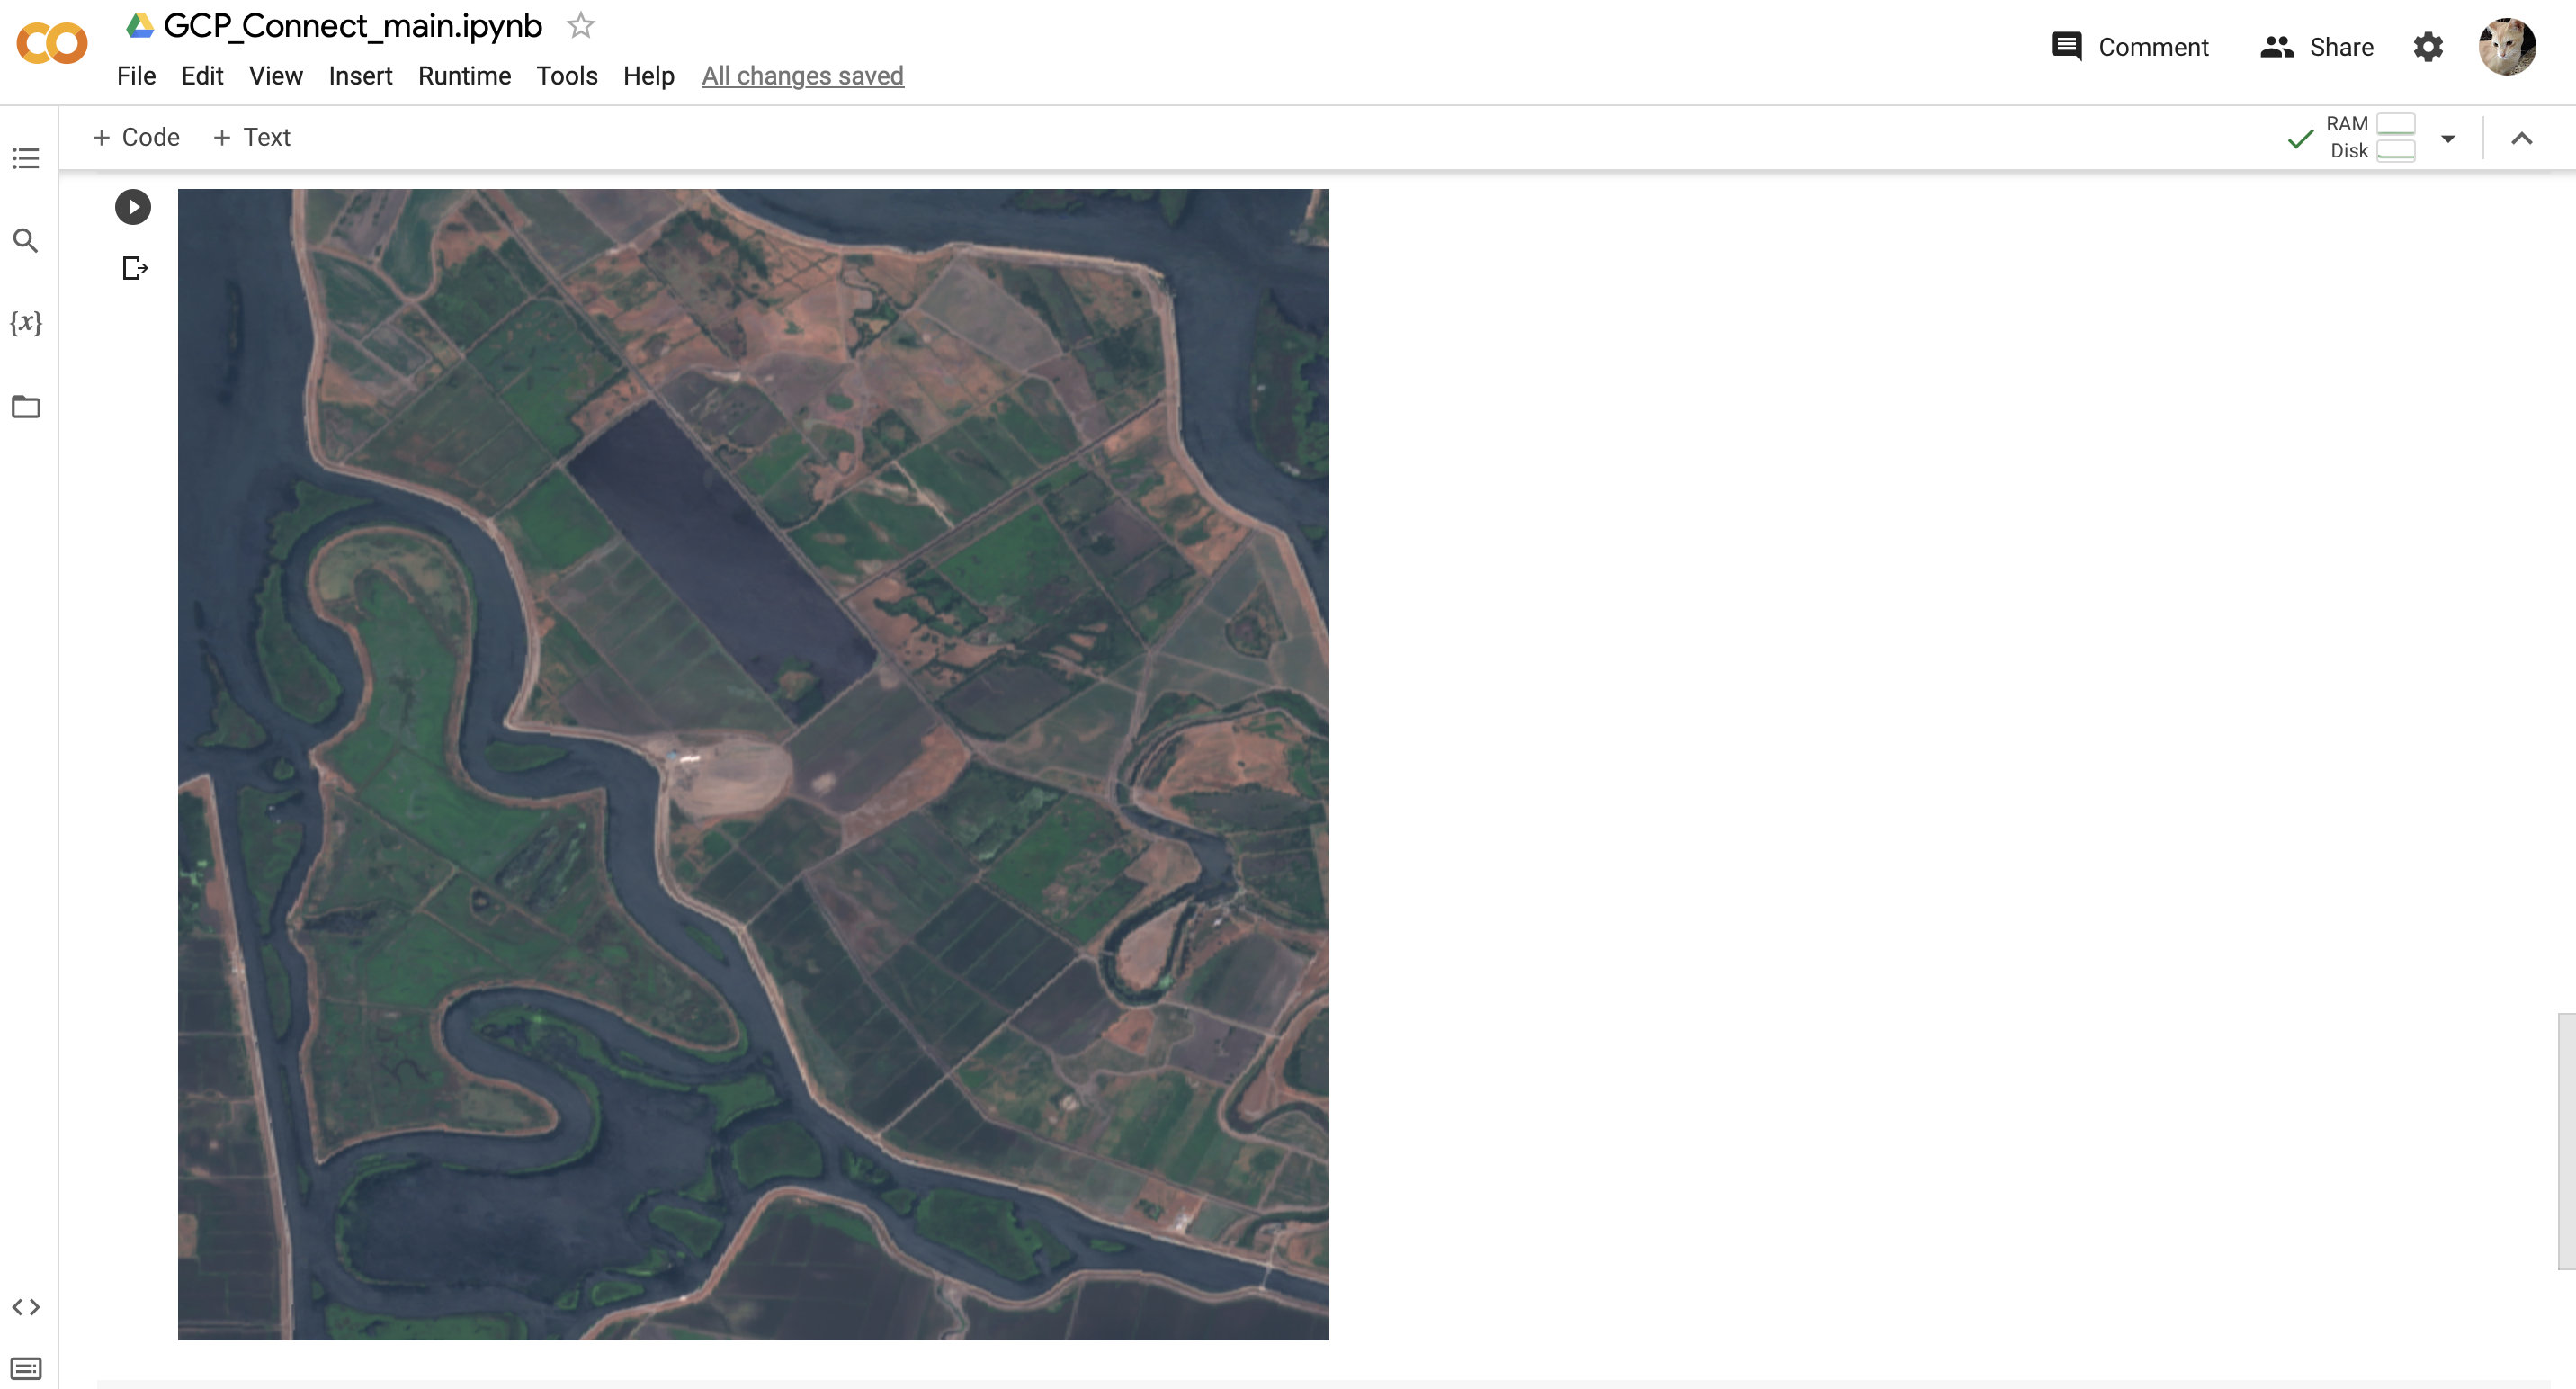
\includegraphics[scale=0.4]{screenshts/18.png}
\chapter{Testing the Model}
\section{Testing the Image from GCP GE}
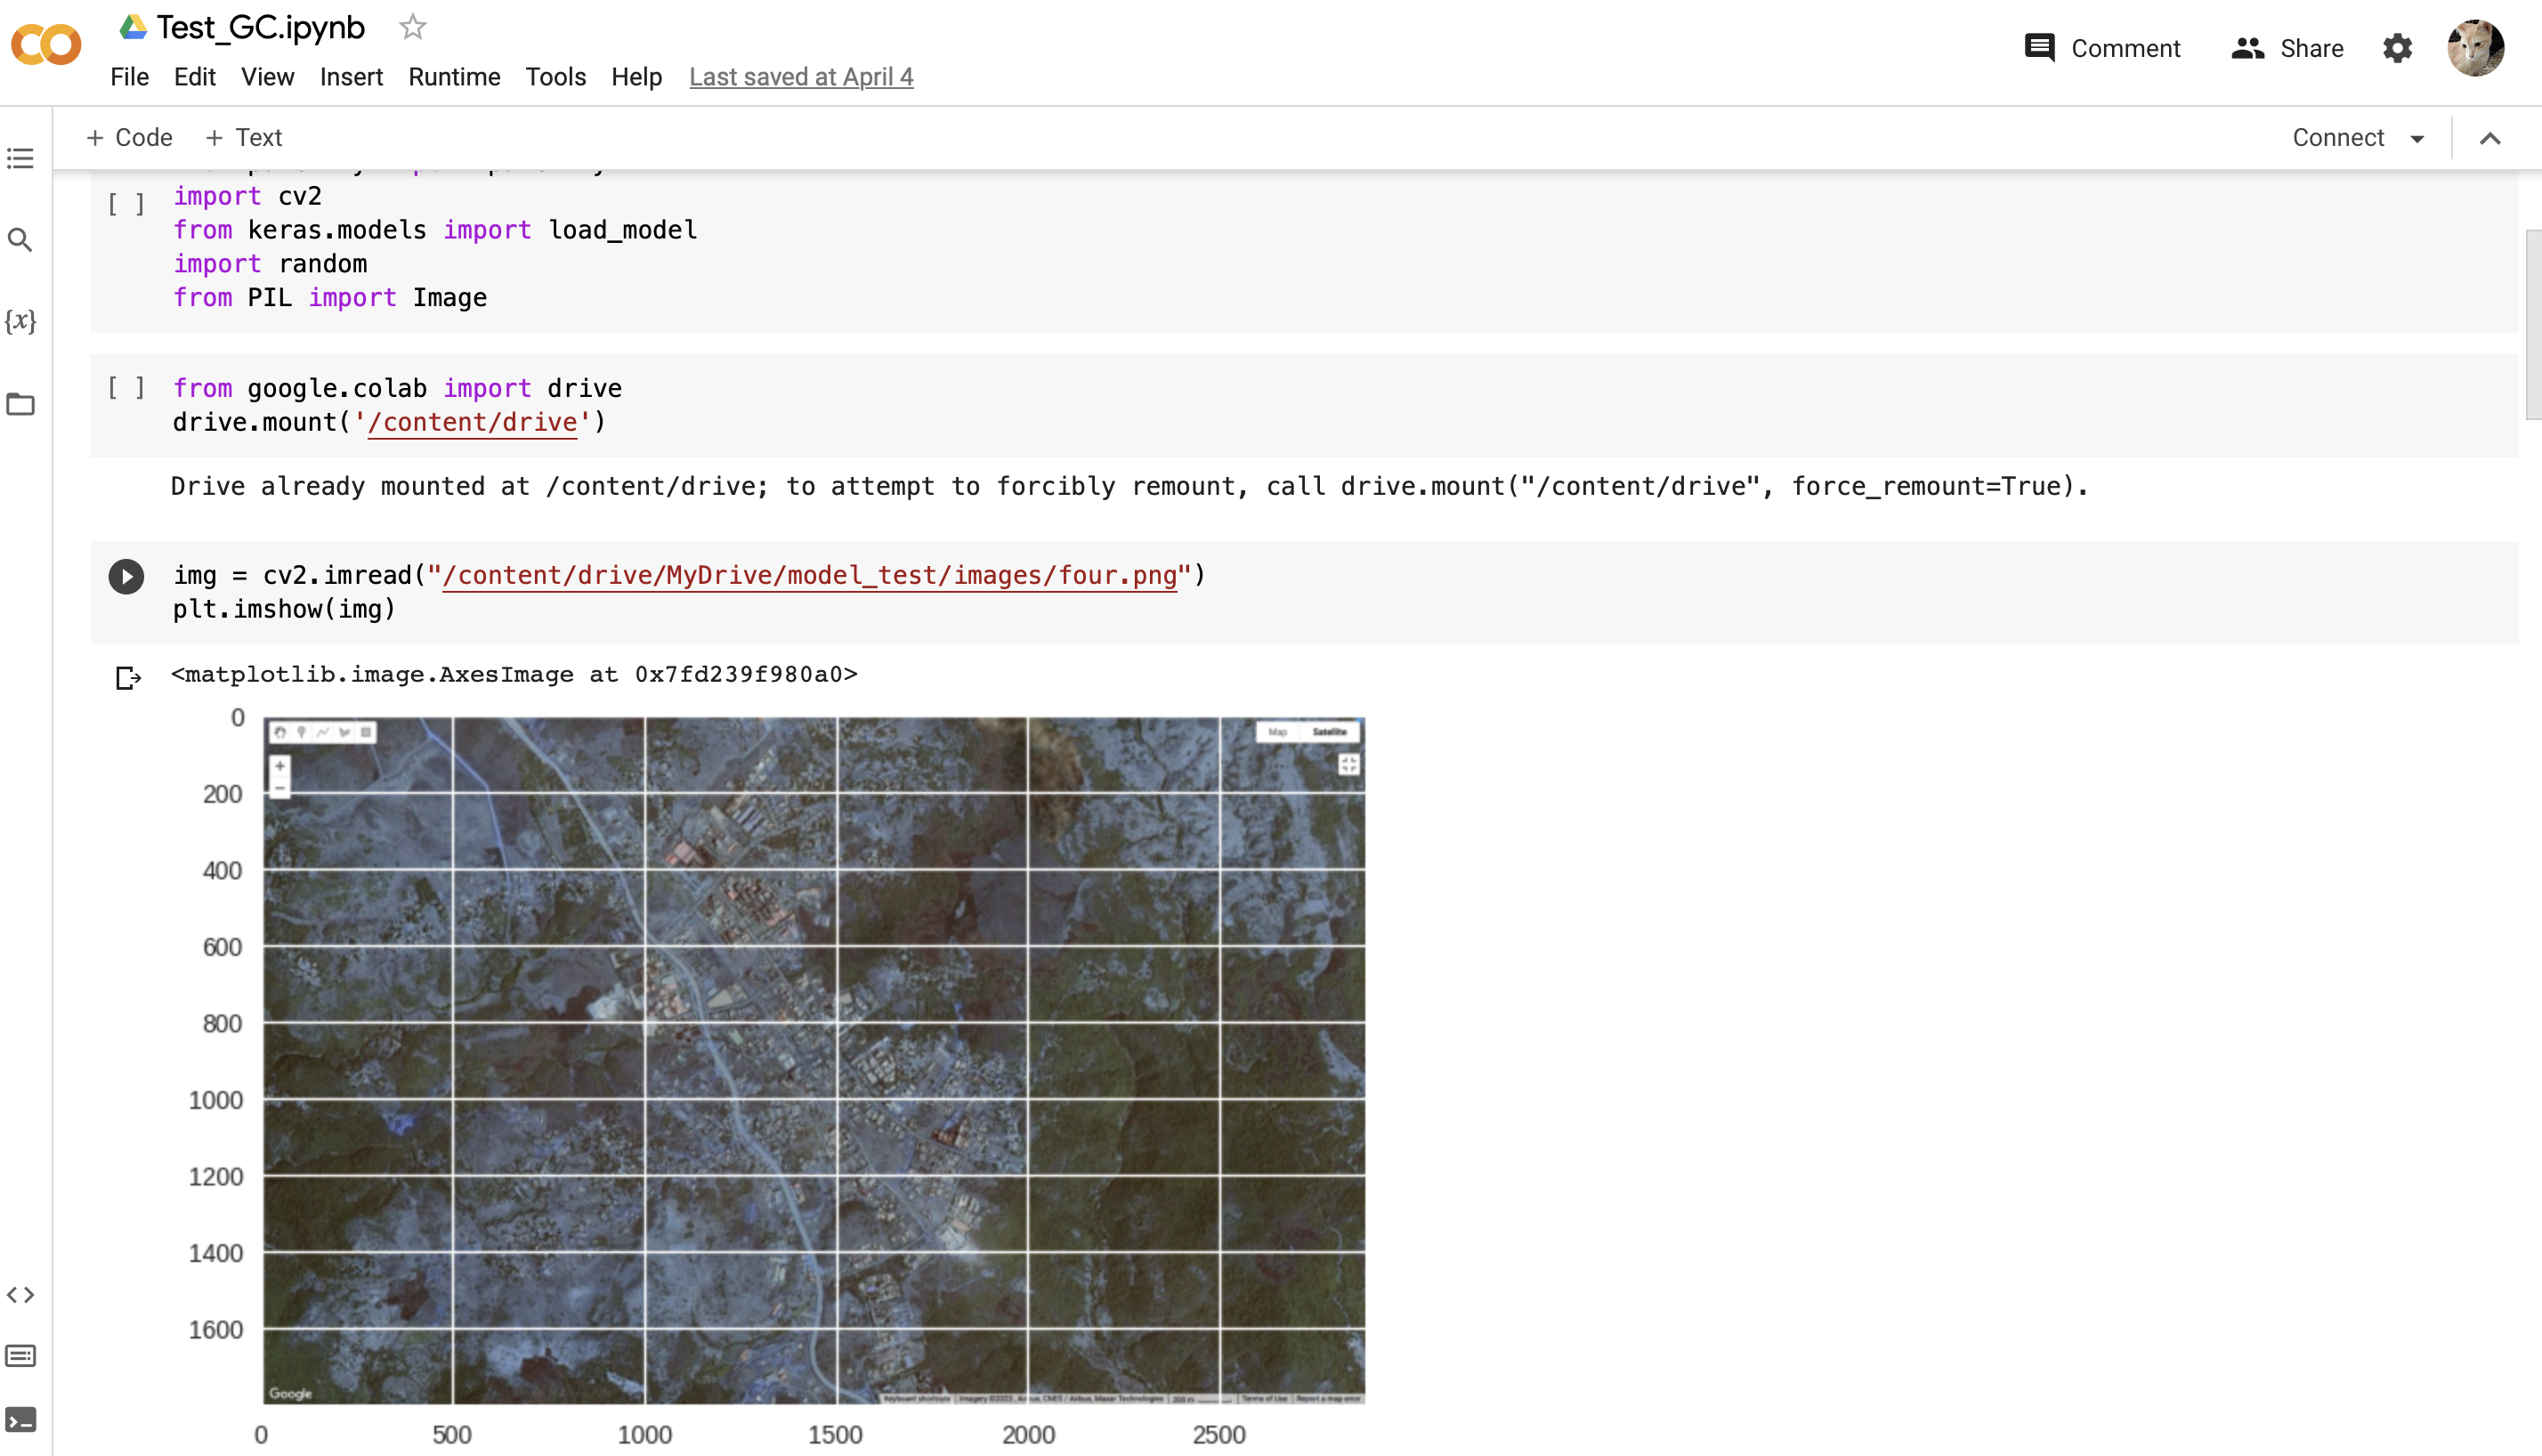
\includegraphics[scale=0.4]{screenshts/19.png}\\\\
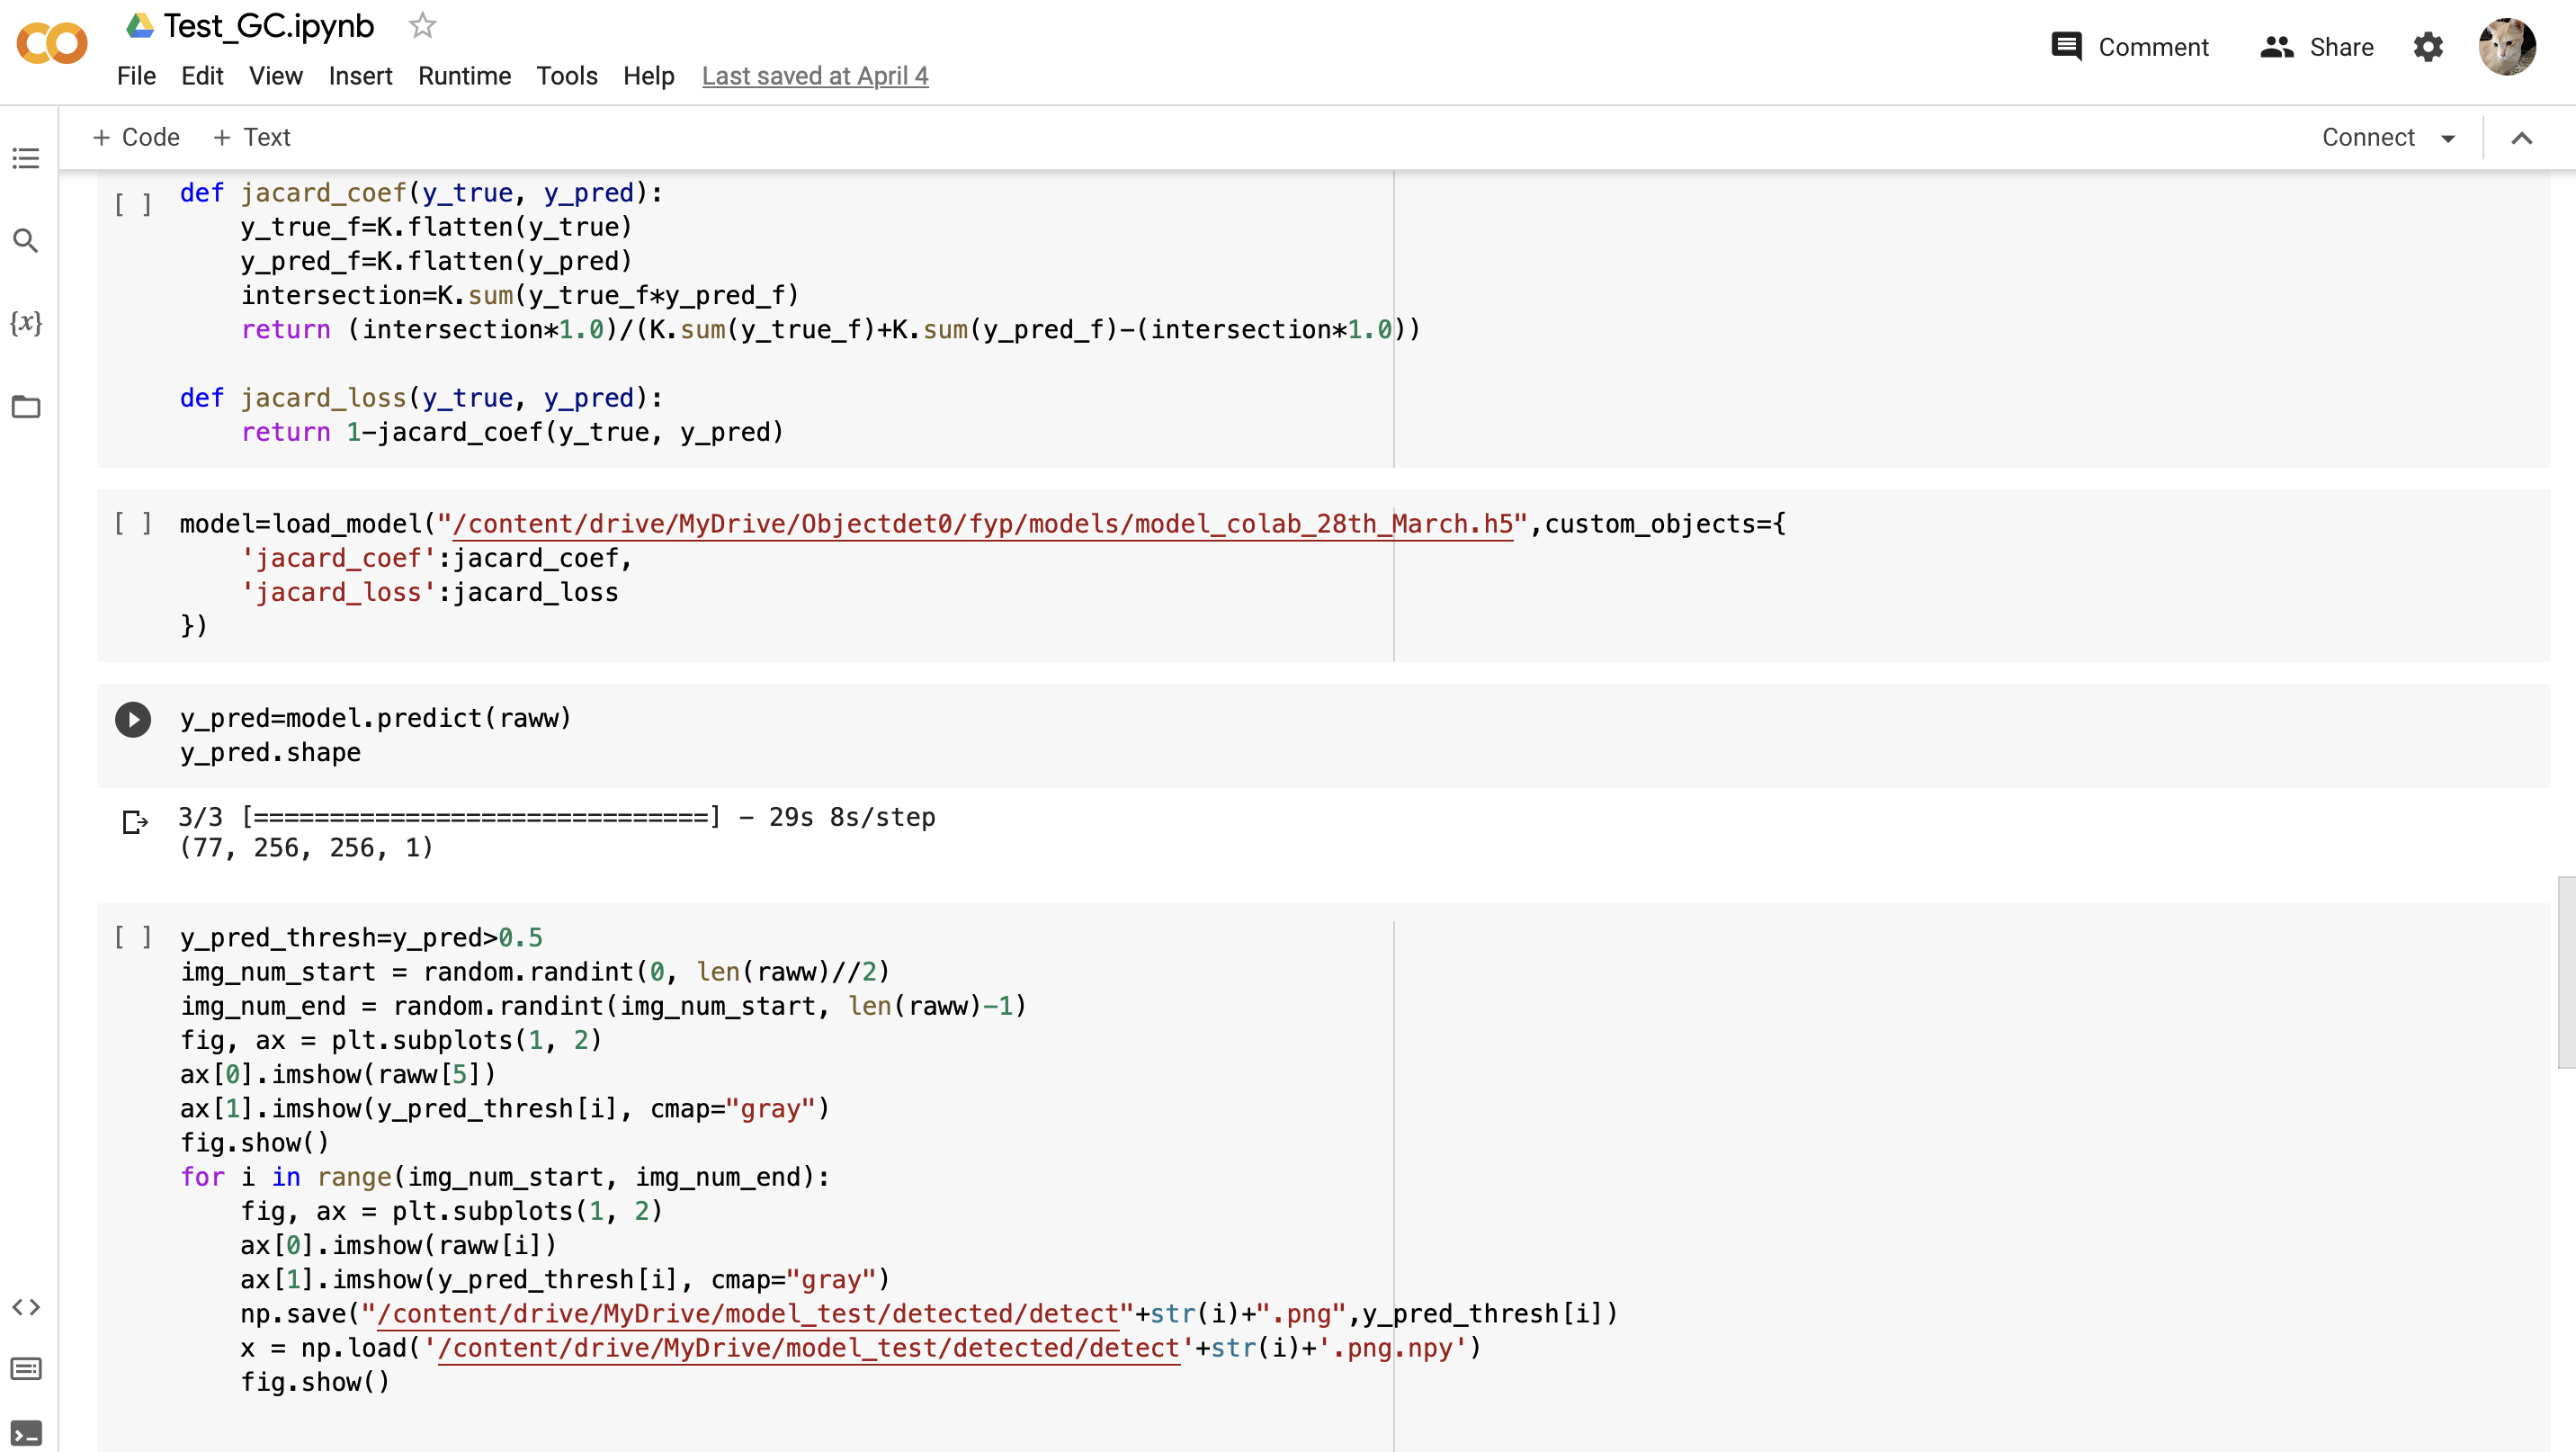
\includegraphics[scale=0.4]{screenshts/20.png}\\\\
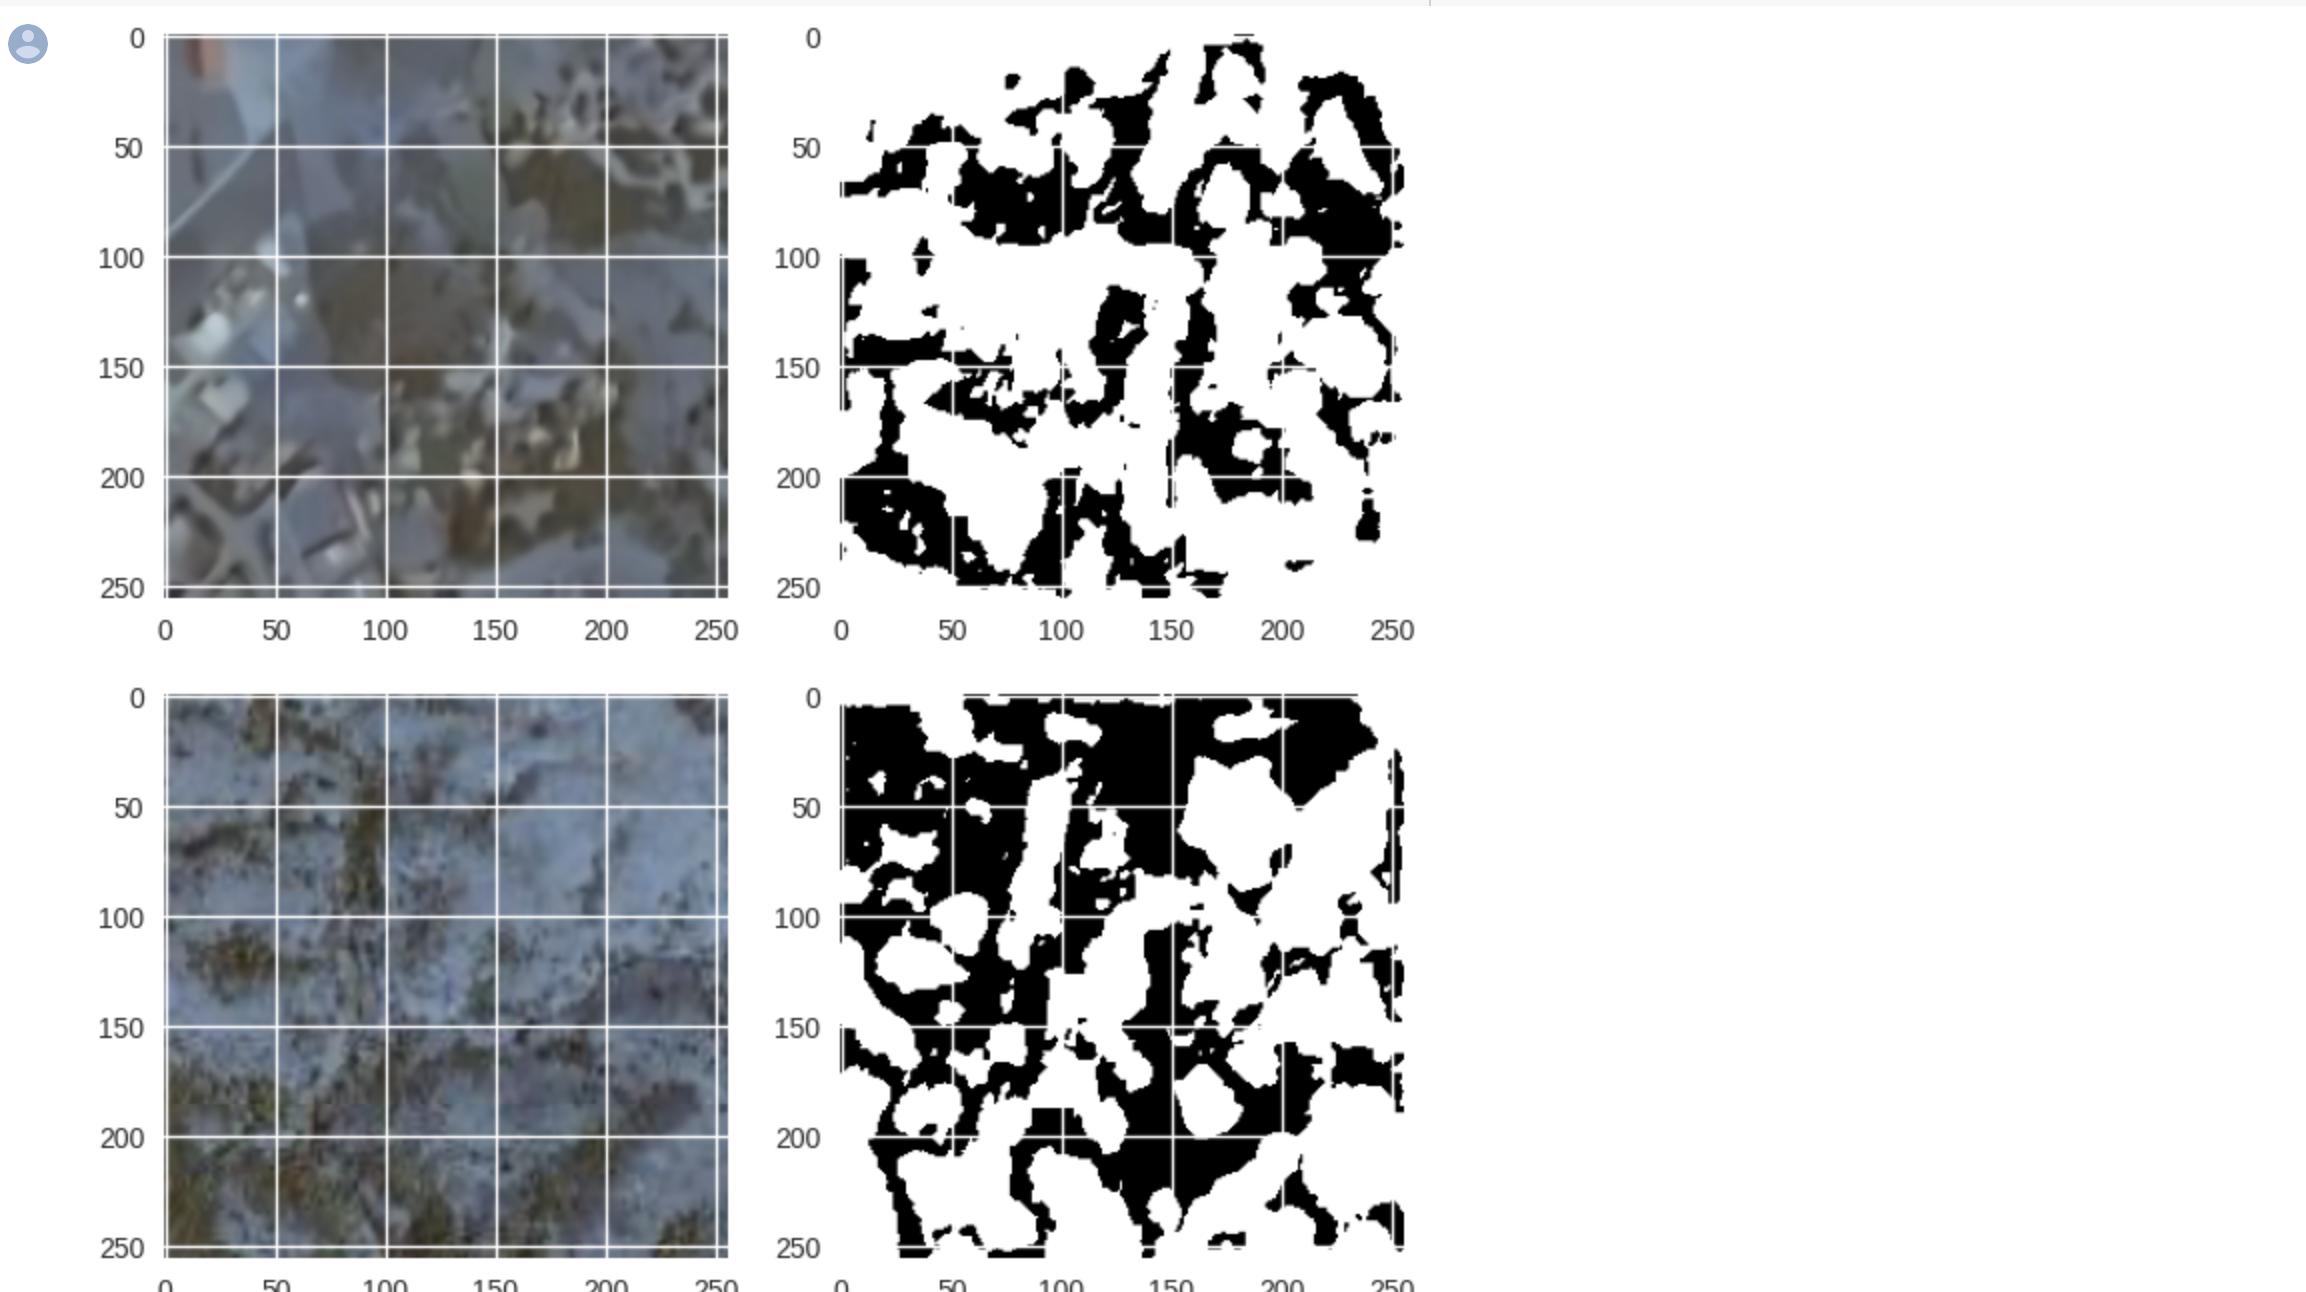
\includegraphics[scale=0.4]{screenshts/21.png}\\\\\\\
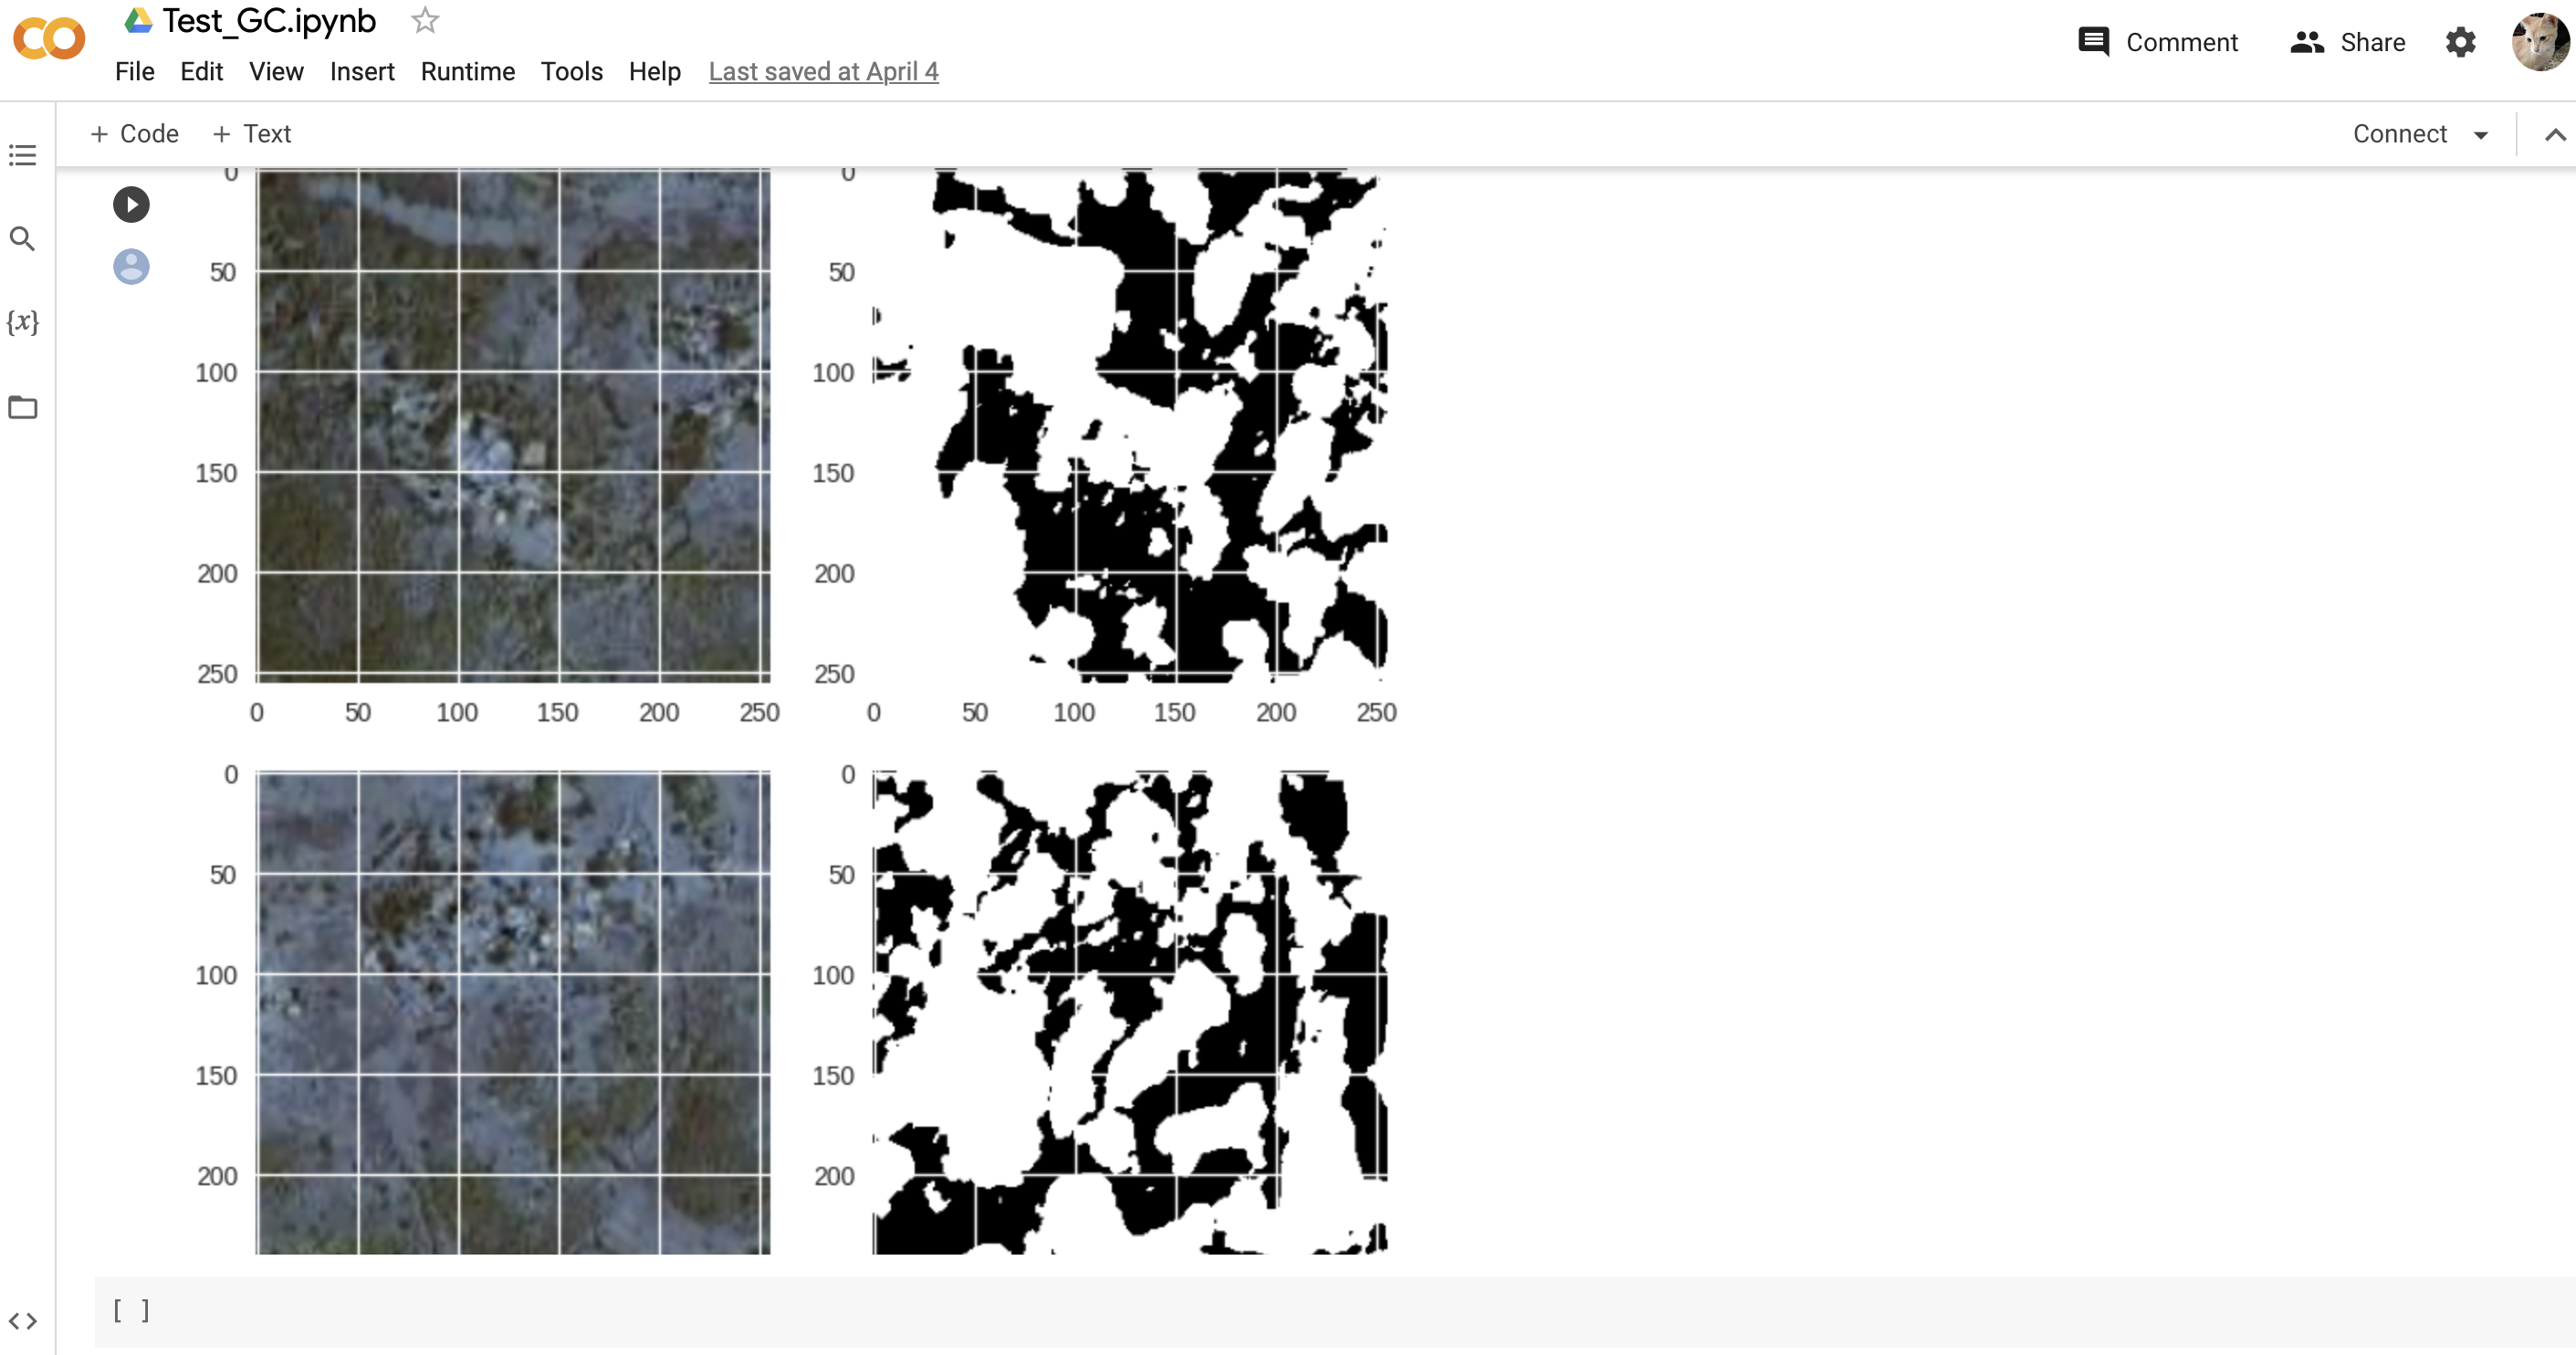
\includegraphics[scale=0.4]{screenshts/22.png}
\chapter{Conclusions and Future Work}
\section{Conclusion}
we can conclude that deep learning techniques can effectively address the challenges of object detection in satellite imagery. The proposed method, which uses a deep learning model based on the Faster R-CNN architecture, achieved higher accuracy and faster processing time compared to other state-of-the-art object detection methods.

The proposed method has several potential applications, including urban planning, environmental monitoring, and disaster response. Future research could focus on improving the accuracy of the model by incorporating additional data sources, such as multi-spectral imagery, and exploring the use of transfer learning to reduce the need for large training datasets.

Overall, my work demonstrates the potential of deep learning techniques for object detection in satellite imagery and highlights the importance of developing new methods to improve the accuracy and efficiency of these techniques for real-world applications.

\section{Future Work}
As for the future work of the project, there are several potential directions that could be explored to further improve the accuracy and applicability of the proposed building detection method.

Firstly, incorporating additional data sources, such as multi-spectral or LiDAR data, could improve the accuracy of the detection method, especially in complex urban environments with high-rise buildings or dense vegetation.

Secondly, exploring transfer learning techniques could reduce the amount of labeled data required for training the model and allow for better generalization to different geographical areas or imaging conditions.

Finally, integrating the building detection method into a larger system for urban planning or disaster response could help to better understand and respond to urban changes and emergencies in real-time.


%Add Chapters as much as you want!
\include{private/list-of-symbols}

\renewcommand*{\bibname}{References}

% Add the References to the Table of Contents
\addcontentsline{toc}{chapter}{\textbf{References}}
%----------------------------------------------------------------------
% APPENDICES
%---------------------------------------------------------------------- 

\addcontentsline{toc}{chapter}{APPENDICES} 
\appendix
% B I B L I O G R A P H Y
% -----------------------

\bibliographystyle{plain}
% This specifies the location of the file containing the bibliographic information.  
% It assumes you're using BibTeX (if not, why not?).
\ifthenelse{\boolean{PrintVersion}}{
\cleardoublepage % This is needed if the book class is used, to place the anchor in the correct page,
                 % because the bibliography will start on its own page.
}{
\clearpage       % Use \clearpage instead if the document class uses the "oneside" argument
}
\phantomsection  % With hyperref package, enables hyperlinking from the table of contents to bibliography             
% The following statement causes the title "References" to be used for the bibliography section:


\bibliography{bibliography/keylatex}
% Tip 5: You can create multiple .bib files to organize your references. 
% Just list them all in the \bibliogaphy command, separated by commas (no spaces).

\include{Chapters/Appendix_A} %"Sources of Information and Help"
% An appendix
%======================================================================
\chapter{Python Implementation}
%======================================================================
\section{Libraries}
\begin{lstlisting}[language=Python]
import matplotlib.pyplot as plt
import numpy as np 
import os
from patchify import patchify
import cv2
from keras.models import load_model
import random
from PIL import Image



#Imports
import os
from google.colab import drive
from PIL import Image
import os
from pathlib import Path
from google.auth.transport.requests import AuthorizedSession
from google.oauth2 import service_account
from pprint import pprint
import json
import ee
from IPython.display import Image


import matplotlib.pyplot as plt
import numpy as np 
import os
from keras.models import load_model
from keras.preprocessing.image import ImageDataGenerator
import cv2
from sklearn.model_selection import train_test_split
from sklearn.preprocessing import MinMaxScaler
from keras.callbacks import ModelCheckpoint, LearningRateScheduler, EarlyStopping
import random



import cv2
import numpy as np
import os
import matplotlib.pyplot as plt
from PIL import Image
from patchify import patchify
import splitfolders
import random
from keras.utils import to_categorical




\end{lstlisting}


\section{Code} 
\subsection{Pre-Processing}
\begin{lstlisting}[language=Python]
from google.colab import drive
drive.mount('/content/drive')
img=cv2.imread("/content/drive/My Drive/Objectdet0/fyp/landcover.ai.v1/images/N-33-60-D-c-4-2.tif")
plt.figure(figsize=(18,10))
plt.subplot(131)
plt.title("R-channel")
print(img)
plt.imshow(img[:,:,0])
plt.subplot(132)

plt.title("G-channel")
plt.imshow(img[:,:,1])
plt.subplot(133)
plt.title("B-channel")
plt.imshow(img[:,:,2])
plt.show()



img=cv2.imread("/content/drive/My Drive/Objectdet0/fyp/landcover.ai.v1/masks/N-33-60-D-c-4-2.tif",0)
print(img.shape)
labels, count=np.unique(img, return_counts=True)
print(labels, count)
n_classes=len(labels)
# converting to categorical data
img=to_categorical(img, num_classes=n_classes)
plt.figure(figsize=(18,18))
for i in range(n_classes):
    plt.subplot(161+i)
    plt.title(f"Channel {i+1}")
    plt.imshow(img[:,:,i])
plt.show()


img=cv2.imread("/content/drive/My Drive/Objectdet0/fyp/landcover.ai.v1/masks/N-33-60-D-c-4-2.tif",0)
# only considereing buildings and converting rest all to unlabelled background
img[img > 1] = 0
print(img.shape)
labels, count=np.unique(img, return_counts=True)
print(labels, count)
n_classes=len(labels)
# converting to categorical data
img=to_categorical(img, num_classes=n_classes)
plt.figure(figsize=(18,18))
for i in range(n_classes):
    plt.subplot(161+i)
    plt.title(f"Channel {i+1}")
    plt.imshow(img[:,:,i])
plt.show()


root_dir = "/content/drive/My Drive/Objectdet0/fyp/landcover.ai.v1/"
patch_size = 256
img_dir = root_dir+"images/"
mask_dir = root_dir+"masks/"
# new_img_dir = root_dir+"256_patches/images/"
# new_mask_dir = root_dir+"256_patches/masks/"
new_img_dir = root_dir+"256_patches_4_classes/images/"
new_mask_dir = root_dir+"256_patches_4_classes/masks/"
try:
    os.makedirs(new_img_dir)
    os.makedirs(new_mask_dir)
except:
    print("Directory already available, so not created")
img_list = sorted(os.listdir(img_dir))
msk_list = sorted(os.listdir(mask_dir))



# the images and masks with decent amout of labels are seperated and used for training.
no_use_images=0
useful_images=0

# save the 256x256 with rules as mentioned above so that they can be used for data augumentation
# resizing will change the size of real image, so divide the image into patches of 256x256x3
for img in range(len(img_list)):
    img_name=img_list[img]
    mask_name=msk_list[img]
    print(f"Analysing {img_name} with {mask_name}")
    if img_name.endswith(".tif") and mask_name.endswith(".tif"):
        # at this point, image and mask variables contains a large sized images
        image=cv2.imread(img_dir+img_name,1)
        mask=cv2.imread(mask_dir+mask_name, 0)
        # here we crop the image so that size is near to the greatest multiple of 256
        size_x = (image.shape[1]//patch_size)*patch_size
        size_y = (image.shape[0]//patch_size)*patch_size
        # converting to pillow image
        image = Image.fromarray(image)
        mask = Image.fromarray(mask)
        # cropping from top left corner
        image = image.crop((0, 0, size_x, size_y))
        mask = mask.crop((0, 0, size_x, size_y))
        image = np.array(image)
        mask = np.array(mask)
        # converting the large image into patches
        patches_image = patchify(image, (patch_size, patch_size, 3), step=patch_size)
        patches_mask = patchify(mask, (patch_size, patch_size), step=patch_size)
        
        # save the patches to local directory
        print(patches_image.shape, patches_mask.shape)
        for i in range(patches_image.shape[0]):
            for j in range(patches_image.shape[1]):
                patch_img = patches_image[i, j, :, :]
                patch_mask = patches_mask[i, j, :, :]
                # dropping the extra part created by patchify
                patch_img = patch_img[0]
                # seggregating useful and useless images
                val, counts=np.unique(patch_mask, return_counts=True)
                # 0th index store count of unlabelled pixels
                # if unlabelled pixels are atmost 95% of total pixels, then we have atleast 5% useful pixels.
                # and also atleast 5% of the mask pixels must be of building class.
                total_pixels=counts.sum()
                count_of_unlabelled_pixel_arr = counts[np.where(val == 0)[0]]
                count_of_building_pixel_arr = counts[np.where(val == 1)[0]]
                count_of_unlabelled_pixel = 0
                count_of_building_pixel = 0
                if(len(count_of_unlabelled_pixel_arr) != 0):
                    count_of_unlabelled_pixel=count_of_unlabelled_pixel_arr[0]
                if(len(count_of_building_pixel_arr) != 0):
                    count_of_building_pixel=count_of_building_pixel_arr[0]

                if(count_of_unlabelled_pixel/total_pixels < 0.95 and 
                    count_of_building_pixel/total_pixels > 0.05):
                    # only considereing buildings and converting rest all to unlabelled background
                    # patch_mask[patch_mask > 1] = 0
                    print(f"Patch {i}-{j} {patch_img.shape}, {patch_mask.shape} generated")
                    new_path_image = os.path.join(
                        new_img_dir, 
                        r"{}".format(img_name.split(".")[0]+'patch_'+str(i)+str(j)+'.tif'))
                    new_path_mask = os.path.join(
                        new_mask_dir, 
                        r"{}".format(mask_name.split(".")[0]+'patch_'+str(i)+str(j)+'.tif'))
                    cv2.imwrite(new_path_image, patch_img)
                    cv2.imwrite(new_path_mask, patch_mask)
                    useful_images+=1
                else:
                    no_use_images+=1





num_images = len(os.listdir(new_img_dir))
img_num = random.randint(0, num_images-1)
print(f'Inspect 1 patch image mask pair out of {num_images}')
new_img_list = sorted(os.listdir(new_img_dir))
new_mask_list = sorted(os.listdir(new_mask_dir))
print(new_img_list[img_num], new_img_list[img_num])
img_for_plot = cv2.imread(new_img_dir+new_img_list[img_num], 1)
mask_for_plot =cv2.imread(new_mask_dir+new_mask_list[img_num], 0)

plt.figure(figsize=(10, 8))
plt.subplot(121)
plt.imshow(img_for_plot)
plt.title('Image')
plt.subplot(122)
plt.imshow(mask_for_plot, cmap='gray')
plt.title('Mask')
plt.show()


\end{lstlisting}


\subsection{Training}
\begin{lstlisting}[language=Python]
seed = 32
root_dir = "/content/drive/My Drive/Objectdet0/fyp/landcover.ai.v1/256_patches/"
patch_size = 256
batch_size = 16
n_classes = 1
new_img_mask_dir = root_dir+"flow_dir/"
# inside train_images folder, we mock the Imagegenerator class that we have 1 class called "images" 
# similarly for all the other three folders.
train_img_dir=new_img_mask_dir+"train_images/"
train_mask_dir=new_img_mask_dir+"train_masks/"
val_img_dir=new_img_mask_dir+"val_images/"
val_mask_dir=new_img_mask_dir+"val_masks/"

img_list = os.listdir(train_img_dir+"images/")
mask_list = os.listdir(train_mask_dir+"masks/")
val_img_list = os.listdir(val_img_dir+"images/")
val_mask_list = os.listdir(val_mask_dir+"masks/")
img_list = sorted(img_list)
mask_list = sorted(mask_list)
val_img_list = sorted(val_img_list)
val_mask_list = sorted(val_mask_list)
steps_per_epoch = len(img_list)//batch_size
val_steps_per_epoch = len(val_img_list)//batch_size



# checking
num_images = len(img_list)
num_masks = len(mask_list)
img_num = random.randint(0, num_images-1)
print(f'Inspect 1 patch image mask pair out of {num_images}')
print(train_img_dir+"images/"+img_list[img_num])
print(train_mask_dir+"masks/"+mask_list[img_num])
img_for_plot = cv2.imread(train_img_dir+"images/"+img_list[img_num], 1)
mask_for_plot = cv2.imread(train_mask_dir+"masks/"+mask_list[img_num], 0)

plt.figure(figsize=(10, 8))
plt.subplot(121)
plt.imshow(img_for_plot)
plt.title('Image')
# plt.subplot(122)#plt.imshow(mask_for_plot, cmap='gray')
# plt.title('Mask')
plt.show()

print('Max value: ', np.amax(mask_for_plot))
print('Image shape: ', mask_for_plot.shape)
print('Pixels in (256,256) img with value 1 :',np.sum(mask_for_plot==1.0))
print('Pixels in (256,256) img with value 0 :',np.sum(mask_for_plot==0.0))
print('Pixels in (256,256) img with value between 0 and 1 :',np.sum(mask_for_plot>0.0)-np.sum(mask_for_plot==1.0))



X = []
for file in img_list:
    img = cv2.imread(train_img_dir+"images/"+file, 1)
    img=img/255.0
    X.append(img)
Y=[]
for file in mask_list:
    mask =cv2.imread(train_mask_dir+"masks/"+file, 0)
    mask=mask/1.0
    Y.append(mask)
print(len(X), len(Y))
# converting to numpy array
X = np.asarray(X)
print(X.shape)
# convert masks to categorical (one hot encoded) data
Y=np.asarray(Y)
# till now, the masks are integer encoded
print(Y.shape)



X_test = []
for file in val_img_list:
    img = cv2.imread(val_img_dir+"images/"+file, 1)
    img=img/255.0
    X_test.append(img)
Y_test =[]
for file in val_mask_list:
    mask =cv2.imread(val_mask_dir+"masks/"+file, 0)
    mask=mask/1.0
    Y_test.append(mask)
print(len(X_test), len(Y_test))
# converting to numpy array
X_test = np.asarray(X_test)
print(X_test.shape)
# convert masks to categorical (one hot encoded) data
Y_test=np.asarray(Y_test)
# till now, the masks are integer encoded
print(Y_test.shape)






from keras import backend as K
from keras import Input
from keras.layers import Lambda, Dropout, Conv2D, MaxPooling2D, Conv2DTranspose, concatenate
from keras.models import Model

# Mean IOU
def jacard_coef(y_true, y_pred):
    y_true_f=K.flatten(y_true)
    y_pred_f=K.flatten(y_pred)
    intersection=K.sum(y_true_f*y_pred_f)
    return (intersection*1.0)/(K.sum(y_true_f)+K.sum(y_pred_f)-(intersection*1.0))

def jacard_loss(y_true, y_pred):
    return 1-jacard_coef(y_true, y_pred)

IMG_WIDTH=256
IMG_HEIGHT=256
IMG_CHANNELS=3

# multi-class semantic segmentation model (0 and 1, so binary class semantic segmentation)
def unet_model(n_classes):
    """ Contraction path, encoding """
    inputs=Input((IMG_WIDTH, IMG_HEIGHT, IMG_CHANNELS))
    # the layers take floating point values. So we have to convert the integers of the pixel values to floating point
    # so we divide all image by 255
    # this is lambda function over the layer
    # inputs=Lambda(lambda x:x/255)(inputs)
    # 64 feature dimensions, kernal size, 
    # he_normal is one kind of provision of starting weights of the neural network. In the process of iteration, the weights get better.
    # this is truncated around 0, and follows gaussian distribution.
    # same padding meanss output image dimensions are same as input image
    # we apply all the conv1 on the inputs layer
    conv1=Conv2D(32,(3,3), activation="relu", kernel_initializer="he_normal", padding="same")(inputs)
    # dropping out 10% of the nodes
    conv1=Dropout(0.2)(conv1)
    conv1=Conv2D(32,(3,3), activation="relu", kernel_initializer="he_normal", padding="same")(conv1)
    
    # pool size=(2,2)
    conv2=MaxPooling2D((2,2))(conv1)
    conv2=Conv2D(64,(3,3), activation="relu", kernel_initializer="he_normal", padding="same")(conv2)
    conv2=Dropout(0.2)(conv2)
    conv2=Conv2D(64,(3,3), activation="relu", kernel_initializer="he_normal", padding="same")(conv2)
    
    conv3=MaxPooling2D((2,2))(conv2)
    conv3=Conv2D(128,(3,3), activation="relu", kernel_initializer="he_normal", padding="same")(conv3)
    conv3=Dropout(0.2)(conv3)
    conv3=Conv2D(128,(3,3), activation="relu", kernel_initializer="he_normal", padding="same")(conv3)
    
    conv4=MaxPooling2D((2,2))(conv3)
    conv4=Conv2D(256,(3,3), activation="relu", kernel_initializer="he_normal", padding="same")(conv4)
    conv4=Dropout(0.2)(conv4)
    conv4=Conv2D(256,(3,3), activation="relu", kernel_initializer="he_normal", padding="same")(conv4)
    
    conv5=MaxPooling2D((2,2))(conv4)
    conv5=Conv2D(512,(3,3), activation="relu", kernel_initializer="he_normal", padding="same")(conv5)
    conv5=Dropout(0.2)(conv5)
    conv5=Conv2D(512,(3,3), activation="relu", kernel_initializer="he_normal", padding="same")(conv5)

    """ Expansion path, decoding """
    upconv6=Conv2DTranspose(256,(2,2), strides=(2,2), padding="same")(conv5)
    upconv6=concatenate([upconv6, conv4])
    conv6=Conv2D(256,(3,3), activation="relu", kernel_initializer="he_normal", padding="same")(upconv6)
    conv6=Dropout(0.2)(conv6)
    conv6=Conv2D(256,(3,3), activation="relu", kernel_initializer="he_normal", padding="same")(conv6)

    upconv7=Conv2DTranspose(128,(2,2), strides=(2,2), padding="same")(conv6)
    upconv7=concatenate([upconv7, conv3])
    conv7=Conv2D(128,(3,3), activation="relu", kernel_initializer="he_normal", padding="same")(upconv7)
    conv7=Dropout(0.2)(conv7)
    conv7=Conv2D(128,(3,3), activation="relu", kernel_initializer="he_normal", padding="same")(conv7)

    upconv8=Conv2DTranspose(64,(2,2), strides=(2,2), padding="same")(conv7)
    upconv8=concatenate([upconv8, conv2])
    conv8=Conv2D(64,(3,3), activation="relu", kernel_initializer="he_normal", padding="same")(upconv8)
    conv8=Dropout(0.2)(conv8)
    conv8=Conv2D(64,(3,3), activation="relu", kernel_initializer="he_normal", padding="same")(conv8)

    upconv9=Conv2DTranspose(32,(2,2), strides=(2,2), padding="same")(conv8)
    upconv9=concatenate([upconv9, conv1])
    conv9=Conv2D(32,(3,3), activation="relu", kernel_initializer="he_normal", padding="same")(upconv9)
    conv9=Dropout(0.2)(conv9)
    conv9=Conv2D(32,(3,3), activation="relu", kernel_initializer="he_normal", padding="same")(conv9)
    
    conv9=Conv2D(16,(3,3), activation="relu", kernel_initializer="he_normal", padding="same")(conv9)
    outputs=Conv2D(n_classes,(1,1), activation="sigmoid", padding="same")(conv9)


    model=Model(inputs=[inputs], outputs=[outputs])

    return model


import keras
from keras.optimizers import Adam
model = unet_model(n_classes)
# optimizer includes the backpropagation algorithms to train the model.
# binary cross entropy is used for binary classification of true or not true situations in segmentaiton.
# optimizer tries to minimize the loss function.
# jacard_coef determined "Intersection Over Union" score
'''
loss=[
        jacard_loss,
        'binary_crossentropy'
    ],
    loss_weights=[1,1],
  metrics=[
        "accuracy", 
        jacard_coef
    ]
'''
model.compile(
    optimizer=Adam(learning_rate = 1e-3), loss=jacard_loss, 
    metrics=['accuracy',jacard_coef]
)




# to avoid overfitting of model
earlystopping = EarlyStopping(
    monitor="val_loss", 
    mode="min", patience=3, 
    restore_best_weights=True
)



# make a new folder to save model
try:
    os.makedirs(root_dir+"models")
except:
    print("Directory already available, so not created")



history = model.fit(
    X,Y,
    steps_per_epoch=steps_per_epoch, 
    epochs=20, 
    verbose=1,
    callbacks=[earlystopping],
    validation_data=(X_test, Y_test),
    validation_steps=val_steps_per_epoch
)



#plot the training and validation accuracy and loss at each epoch
loss = history.history['loss']
val_loss = history.history['val_loss']
epochs = range(1, len(loss) + 1)
plt.plot(epochs, loss, 'y', label='Training loss')
plt.plot(epochs, val_loss, 'r', label='Validation loss')
plt.title('Training and validation loss')
plt.xlabel('Epochs')
plt.ylabel('Loss')
plt.legend()
plt.show()

acc = history.history['accuracy']
val_acc = history.history['val_accuracy']
plt.plot(epochs, acc, 'y', label='Training acc')
plt.plot(epochs, val_acc, 'r', label='Validation acc')
plt.title('Training and validation accuracy')
plt.xlabel('Epochs')
plt.ylabel('Accuracy')
plt.legend()
plt.show()


from keras.metrics import MeanIoU
n_classes = 2
IOU_keras = MeanIoU(num_classes=n_classes)  
IOU_keras.update_state(y_pred_thresh, Y_test)
print("Mean IoU =", IOU_keras.result().numpy())




# IOU for individual class
values = np.array(IOU_keras.get_weights()).reshape(n_classes, n_classes)
print(values)
print("\n")
class0_IOU = values[0,0]/(values[0,0]+values[0,1])
class1_IOU = values[1,1]/(values[1,0]+values[1,1])
print("Unlabelled IOU: ", class0_IOU)
print("Buildings IOU: ", class1_IOU)




for i in range(11,30):
    fig, ax = plt.subplots(1, 3)
    ax[0].imshow(X_test[i])
    ax[1].imshow(Y_test[i], cmap="gray")
    ax[2].imshow(y_pred_thresh[i],  cmap="gray")
    fig.show()




\end{lstlisting}


\subsection{GCP Connection GE API}
\begin{lstlisting}[language=Python]

PROJECT = 'objectdet0'

!gcloud auth login --project {PROJECT}

SERVICE_ACCOUNT='sujay-gcp@objectdet0.iam.gserviceaccount.com'
KEY = 'key.json'

!gcloud iam service-accounts keys create {KEY} --iam-account {SERVICE_ACCOUNT}


from google.auth.transport.requests import AuthorizedSession
from google.oauth2 import service_account

credentials = service_account.Credentials.from_service_account_file(KEY)
scoped_credentials = credentials.with_scopes(
    ['https://www.googleapis.com/auth/cloud-platform'])

session = AuthorizedSession(scoped_credentials)

url = 'https://earthengine.googleapis.com/v1beta/projects/earthengine-public/assets/LANDSAT'

response = session.get(url)

from pprint import pprint
import json
pprint(json.loads(response.content))

import ee

# Get some new credentials since the other ones are cloud scope.
ee_creds = ee.ServiceAccountCredentials(SERVICE_ACCOUNT, KEY)
ee.Initialize(ee_creds)


coords = [
  -121.58626826832939, 
  38.059141484827485,
]
region = ee.Geometry.Point(coords)

collection = ee.ImageCollection('COPERNICUS/S2')
collection = collection.filterBounds(region)
collection = collection.filterDate('2020-04-01', '2020-09-01')
image = collection.median()


serialized = ee.serializer.encode(image)

# Make a projection to discover the scale in degrees.
proj = ee.Projection('EPSG:4326').atScale(10).getInfo()

# Get scales out of the transform.
scale_x = proj['transform'][0]
scale_y = -proj['transform'][4]




url = 'https://earthengine.googleapis.com/v1beta/projects/{}/image:computePixels'
url = url.format(PROJECT)

response = session.post(
  url=url,
  data=json.dumps({
    'expression': serialized,
    'fileFormat': 'PNG',
    'bandIds': ['B4','B3','B2'],
    'grid': {
      'dimensions': {
        'width': 256,
        'height': 256
      },
      'affineTransform': {
        'scaleX': scale_x,
        'shearX': 0,
        'translateX': coords[0],
        'shearY': 0,
        'scaleY': scale_y,
        'translateY': coords[1]
      },
      'crsCode': 'EPSG:4326',
    },
    'visualizationOptions': {'ranges': [{'min': 0, 'max': 3000}]},
  })
)

image_content = response.content


# Import the Image function from the IPython.display module. 
Image(image_content)



drive.mount('/content/drive')
path = r"/content/drive/MyDrive/model_test/images"
os.chdir(path)
with open(path+"/image.png", "wb") as img:
    img.write(image_content)




\end{lstlisting} %"Matlab Code for Making a PDF Plot"


\end{document}
